\documentclass[a4paper,12pt,fleqn]{report}
\usepackage{epsf}
\linespread{1.3}    
\usepackage{psfig}
\usepackage{url}
\usepackage{graphicx}
\usepackage{wrapfig}
\usepackage{lscape}
\usepackage{rotating}
\usepackage{epstopdf}
\usepackage{subcaption}
\usepackage[utf8x]{inputenc}
\usepackage[T1]{fontenc}
\usepackage[english]{babel}
\usepackage[comma]{natbib}
\usepackage{csvsimple}
\usepackage[toc,page]{appendix}
\usepackage{afterpage}
\usepackage{svg}
\usepackage[section]{placeins}
\usepackage{csquotes}
\usepackage{float}

% Insert a black page after the cover page
\newcommand\blankpage{%
    \null
    \thispagestyle{empty}%
    \addtocounter{page}{-1}%
    \newpage}
    

%
% the following package is for displaying code fragments
%
\usepackage{listings}
\usepackage{color}
\usepackage{xcolor}
 
\definecolor{codegreen}{rgb}{0,0.6,0}
\definecolor{codegray}{rgb}{0.5,0.5,0.5}
\definecolor{codepurple}{rgb}{0.58,0,0.82}
\definecolor{backcolour}{rgb}{0.95,0.95,0.92}
 
%\renewcommand{\lstlistingname}{Code Fragments}% Listing -> Algorithm
\lstdefinestyle{blockstyle}{
    backgroundcolor=\color{backcolour},   
    commentstyle=\color{codegreen},
    keywordstyle=\color{magenta},
    numberstyle=\tiny\color{codegray},
    stringstyle=\color{codepurple},
    basicstyle=\footnotesize,
    breakatwhitespace=false,         
    breaklines=true,                 
    captionpos=b,                    
    keepspaces=true,                 
    numbers=left,                    
    numbersep=5pt,                  
    showspaces=false,                
    showstringspaces=false,
    showtabs=false,                  
    tabsize=2
}

\lstdefinestyle{linestyle}{
    backgroundcolor=\color{backcolour},   
    commentstyle=\color{codegreen},
    keywordstyle=\color{magenta},
    stringstyle=\color{codepurple},
    basicstyle=\footnotesize,
    breakatwhitespace=false,         
    breaklines=true,
    captionpos=b,
    numbers=none,                   
    keepspaces=true,                                                  
    showspaces=false,                
    showstringspaces=false,
    showtabs=false,                  
    tabsize=2
}

\lstdefinestyle{BashInputStyle}{
  language=bash,
  basicstyle=\small\sffamily,
  numbers=left,
  numberstyle=\tiny,
  numbersep=3pt,
  frame=tb,
  columns=fullflexible,
  backgroundcolor=\color{gray!20},
  linewidth=0.9\linewidth,
  xleftmargin=0.1\linewidth
}
 
\lstset{style=blockstyle}

\setlength{\textheight}{8.5in}
\setlength{\oddsidemargin}{0.7in}
\setlength{\evensidemargin}{0.7in}
\setlength{\textwidth}{5.50in}
\setlength{\topmargin}{0.0in}
\setlength{\headheight}{0in}
\setlength{\headsep}{0in}
%\setlength{\parindent}{12mm}
% paragraph indent
\setlength{\parindent}{0pt}
% spacing between paragraphs
\setlength{\parskip}{1ex plus 0.5ex minus 0.2ex}

% To have pagenumbering for abstract, we may renew abstract

\makeatletter
\if@titlepage
  \renewenvironment{abstract}{%
%      \titlepage
      \null\vfil
      \@beginparpenalty\@lowpenalty
      \begin{center}%
        \bfseries \abstractname
        \@endparpenalty\@M
      \end{center}}%
     {\par\vfil\null  %\endtitlepage
     }
\else
  \renewenvironment{abstract}{%
      \if@twocolumn
        \section*{\abstractname}%
      \else
        \small
        \begin{center}%
          {\bfseries \abstractname\vspace{-.5em}\vspace{\z@}}%
        \end{center}%
        \quotation
      \fi}
      {\if@twocolumn\else\endquotation\fi}
\fi
\makeatother


%\usepackage{thesis}
\pagestyle{plain}

\begin{document}

\begin{titlepage}
    \begin{center}
        \vspace*{0.5cm}
        
        \Huge
        \textbf{Using Message Passing Interface(MPI) to Parallelise a Simple Genetic Algorithm(SGA) Running on Beowulf Cluster}
        
        \vspace{0.5cm}
        
        
\includegraphics[width=10cm]{figs/UL_Logo.jpeg} \\
        \large
        {\fontfamily{cmss} \selectfont
        Department of CSIS} \\
        \vspace{0.8cm}
        \large
        \textsc{Final Year Project} - 2017 \\
        By: \textbf{Abdul Halim} \\
        ID: 13029096 \\
         \vspace{1cm}
        %\LARGE
        
        \vfill
        \textbf{Bachelor of Science in Computer Systems (LM051)} \\  
        \vspace{0.8cm}
        \normalsize
        \vspace{1cm}
        Supervised by: \textsc{\textbf{J. J. Collins}}
    \end{center}
\end{titlepage}
\afterpage{\blankpage}

%\title{Using Message Passing Interface(MPI) to Parallelise a Simple Genetic Algorithm(SGA) Running on Beowulf Cluster}
%\maketitle
%\author{Abdul Halim}
%{\textbf {\footnotesize Supervised by: first name, second name}} \\
%Department CSIS\\
%{\textbf {University of Limerick}}
%\date{}
%
\includegraphics[width=5cm]{figs/UL_Logo.jpg}
\newpage
\pagenumbering{roman}
\pagestyle{plain}
\addcontentsline{toc}{section}{Abstract}
\begin{abstract}
The aim of this project was to leverage Message Passing Interface(MPI) API for the parallelisation of a machine learning paradigm running on a distributed-memory model infrastructure. This High Performance Computing (HPC) architecture is a Beowulf cluster based on commodity hardware and open source software. MPI defines a set of library routines and environment variables to facilitate execution of tasks in parallel across computing nodes using communication and synchronisation constructs.  The Machine Learning paradigm is a Simple Genetic Algorithm (SGA), an adaptive heuristic search and optimisation algorithms based on evolutionary ideas of natural selection and genetics, used for function optimisation in this work. Empirical results are presented on the performance gain using the Beowulf cluster. The findings demonstrate the challenges faced by programmers when trying to balance the communication overhead in MPI and computational complexity when parallelising a program using MPI.
\end{abstract}
\pagebreak













\pagebreak
\afterpage{\blankpage}

\newpage
\setcounter{page}{2} % This has been added
\addcontentsline{toc}{section}{Acknowledgement}
\renewcommand{\abstractname}{Acknowledgement}
\begin{abstract}
First of all, I would like to thank my supervisor J. J. Collins for introducing me this challenging project and providing excellent guidance and support throughout. Without these support and guidance this project would have been nearly impossible to show any substantial outcome.

I want to thank Dr. Norah Power for giving me the opportunity to study this course in CSIS department. I remember the day when I submitted my application for admission still unsure whether I would be accepted or not. And the day when Dr. Power met us in this department for a introduction and a confirmed of a place.

I also want to thank Mr. Tom Mulcahy of Intel Shannon for believing in me and awarding me the \textbf{\textit{Intel Shannon Paul Whelan Scholarship}}. Having received this scholarship meant a lot. It kept my motivation strong throughout.

Many thanks to my family and friends that supported me doing this difficult course for four long years as a mature student. It was a very long journey but I know it is worth every single moment that I spent in this University. I hope you all can forgive me for being so distant sometimes. I hope I can make it up to you all.

Thanks to Josh, Enda, Ben, Angie, Seun, David, Ankit just to name a few that I have had the pleasure to work with as a team on many projects.

Last but not least, a BIG thanks to all CSIS academics and staff members. \newline \newline

\textit{All my works are dedicated to my two little stars; Lamya and Ayaan.}

\end{abstract}
\clearpage
\pagebreak
\afterpage{\blankpage}

\newpage
\setcounter{page}{3} % This has been added
\addcontentsline{toc}{section}{Declaration}
\renewcommand{\abstractname}{Declaration}
\begin{abstract}
I declare that this is my work and all contributions from other persons have been appropriately identified and acknowledged.
\end{abstract}
\clearpage
\pagebreak
\afterpage{\blankpage}

%
% Table Of Contents
%
\newpage
\setcounter{page}{4} 
\tableofcontents

%
% List of figures
%
\listoffigures
\addcontentsline{toc}{section}{List of figures}
%
% List of tables
%
\listoftables
\addcontentsline{toc}{section}{List of tables}
\pagenumbering{arabic}
\setcounter{page}{1}
\chapter{Introduction}
\label{intro}
\section{Summary}
This project explores the Message Passing Interface (MPI) parallel programming paradigm targeting a distributed memory architecture. A Simple Genetic Algorithm (SGA) is parallelised using MPI and deployed on a cluster. An empirically-based analysis of the performance is then presented.

From the early days, computers were traditionally programmed to execute instructions sequentially. Software Engineers have traditionally relied on Moore's Law \citep{Sutter:05} to satisfy their requirement for performance for their serial programs. Moore's Law \citep{schaller1997moore} states that there is a doubling of the transistor count every 18th months, an effective doubling of the workload that the CPU can accommodate . However, it is becoming more difficult to dissipate the heat from chips with increasing transistor count\citep{kim2003leakage}. An alternative approach \citep{Sutter:05} is to increase the number of cores and run them at slower clock speeds. Programmers are now faced with the challenge of parallelising their serial application in order to exploit the parallel deployment infrastructure.

Todays, a smart phones in one's hand packs more computing power than some supercomputers in 1960's. Multi-core systems are everywhere. The biggest challenge programmers face today is utilising these computing power efficiently and effectively. There are some problems that can only be addressed using parallel processing.

Parallel processing is the execution of a program instructions among multiple processors concurrently with the objective of running it in less time\citep{Barney:16}. Parallelism is an important aspect in computing because we no longer live in a world where we could just expect that the Moore's Law will take care of all of the performance needs. Processor's clock speed are not getting much faster as it used to be in years before. The transistors sizes are shrunk so much that we are now facing the challenges on physical limitation of matter and laws of the universe. Increasing clock speed is no longer a viable solution for improve computing performance. In his infamous article titled \textit{"The Free Lunch Is Over"} Herb Sutter went on a great details why it is not possible to add on more clock speed on the processors any longer\citep{Sutter:05}. Hardware vendors shifted their focus on adding more processing cores in a single silicon die to add more speed. But using these cores in an efficient and scalable manner can be very challenging.

Further more, many problems are so large and/or complex that  it is impractical or impossible to solve them on a single machine. Parallel processing is essential for modelling and simulating real world phenomena. These problems are too complex and large to process sequentially.

Parallel solutions sought for problems that demand speed, process a huge amount of data, time-sensitive or time-critical(real time) \citep{Barney:16}. In general, any problems that is computation greedy better suited for parallel implementation. But not all programs are suitable for executing in this manner. In order to execute a program in parallel it must have some regions that can be executed concurrently without affecting the end result \citep{Sutter:05}. There are number of challenges in parallel programming. These challenges include finding concurrency in a program, tasks decomposition \& scheduling, synchronisation \& communication, scaling and debugging \citep{Sutter:05}  . As part of learning the parallel programming paradigm it was intended to research on these challenges and explore the techniques and best practices available.

Genetic Algorithms(GAs) are adaptive heuristic search and optimisation algorithms based on evolutionary ideas of natural selection and genetics\citep{Goldberg:89}. GAs powerful search and optimisation techniques are found to be very useful and effective for solving problems in many different disciplines. GAs have a wide range of interesting application area from machine learning to robotics, engineering design, financial and investment decision making\citep{konfrst:04para}. There are many aspects in GAs that can take advantages of parallel processing for improving performance and efficiency and better results. Parallel implementation of GAs promise a substantial gains in performance\citep{cantu:98}.

Computer cluster is group of computers connected to a local area network that can run parallel applications\citep{Gropp:beowulf}. Beowulf cluster is a parallel computing infrastructure that originated with the idea of processing tasks in parallel by leveraging commodity hardware and open source software\citep{Beowulf.org}.
 
This project is aimed at parallelising a sequential SGA to run on a distributed-memory model parallel environment - Beowulf cluster, using Message Passing Interface (MPI), and analyse the performance. MPI is a standard specification for Message-Passing parallel programming model for distributed-memory system in which data is moved from one process?s address space to another through cooperative message exchange \citep{Gropp:99}. For this project a Beowulf cluster was implemented. At first, the Beowulf was simulated on a VirtualBox in a portable computer. Later on, the cluster was implemented using inexpensive commodity hardware. The popular MPI implementation MPICH4.0 was installed in both setup to provide the MPI environment to compile and run parallel GA's for this project. This involved carrying out other required installation, configuring and administrative tasks on Ubuntu Server 16.04 Linux distribution.

\section{Objectives}
The primary objectives are twofold:
\begin{enumerate}
	\item Parallelise a Simple Genetic Algorithm using MPI for deployment on a distributed memory architecture such as a Beowulf cluster, and
	\item Profile  the performance when free parameters are modified such as the number of nodes in the cluster and population size of the SGA.
\end{enumerate}

Since this project spans to a dimension that covers quite few challenging topics in computing, the secondary objectives of this projects are listed as below:
\begin{itemize}
	\item Implementing and administering Beowulf Cluster
	\item Learning about parallel computing technology
	\item Learning about parallel programming techniques
	\item Study of Message-Passing-Interface(MPI) API
	\item Study of OpenMP API
	\item Exploring Simple Genetic Algorithms
	\item Exploring the parallelisation techniques of GAs
\end{itemize}

\section{Contributions}
This author is not aware of any other existing parallel Genetic Algorithm implementation using Message Passing Interface. The work done on parallelising GA in this project and carried out empirical studies on performance by varying population size on a Beowulf cluster is thought to be first in this field.


\section{Methodology}
The following methodology were adapted for this project:

\begin{enumerate}
	\item Define the research question
	
	The first step into this project was to identify what is the research question that this project is going to answer. There are many aspects in a parallel implementation of SGA to experiment with. We identified how the performance of a parallel GA reflects in terms of number of processes and in terms of population size.
	\item Systematic Literature Review
	
The next step is to identify and select articles, books and Internet resources that are relevant for this project. This is how one carries out research on the topics of Parallelisation, Cluster computing, OpenMP and MPI, and Genetic Algorithms.

	\item Propose a working hypothesis
	
	\item Define parameter of the empirical study clearly specify the objectives of each test case
	
	\item Build the prototype necessary to generate the data for the empirical study
	\item Run the experiments and capture the data
	\item Analyse the results to see if they answer the research question by supporting the working hypothesis.
	\begin{enumerate}
		\item If not, go back to step 3.
		\item If new results are obtained, go back to step 1.
	\end{enumerate}
\end{enumerate}



\section{Overview of the Report}
This report is broken into few major sections.
\paragraph{Introduction}
This section contains a basic overview of the project, objectives, motivations and a brief discussions on other contributions related to this project.
\paragraph {Background Research}
This section discusses the findings of existing research in the area of parallel computing, OpenMP, MPI, Simple Genetic Algorithms and Parallel Genetic Algorithms.
\paragraph {Design and Implementation}
This section describes the design and implementation part of the project under taken. It covers the steps of implementing Beowulf clusters, Parallel implementation of Simple Genetic Algorithms, product development tools and techniques.
\paragraph {Empirical Studies}
This section contains the findings and comparative analysis of performance of implemented parallel GA's on Beowulf cluster.
\paragraph {Discussion and Conclusions}
This section contains the discussions on findings in empirical studies and conclusions.


\section{Motivation}
During my Co-Operative(COOP) education placement at Intel I worked with teams on a number projects on computational intensive network packet processing. These application demand fully utilising the multi-core Intel Xeon processors for increased throughput. While in there I also came across many other projects in the area of Software Defined Networking(SDN) and Network Function Virtualisation(NFV). Even though each projects were different in their own field, one thing were common. These projects were addressing a common aspect; how to increase the data processing performance. The obvious answer to this question is parallel processing and multi-threading. Programmer must be able to write parallel programs to take advantage of these multi-core systems.

I realised the importance of the parallel programming while working on these real world projects at my COOP placements. My main motivation for this project is to learn about parallel programming.

I am also interested on Evolutionary Algorithms and their application in computation. While studying Intelligent System(CS4006) module for this course we were introduced to Genetic Algorithms. Prior to that I had no idea how the evolutionary theories can be applied to find solution that otherwise impossible to find or too costly. For that module I worked on an individual project on optimal visualisation of graph using Simple Genetic Algorithms which I enjoyed very much.

When I found this project on the FYP proposal list, I approached my supervisor to express my interests on this project. However, this project involves implementing MPI on Beowulf cluster. Neither of these terms I was familiar with. But I was equally excited to learn about cluster computing and programming using MPI. I saw this as a great opportunity to step into the High Performance Computing area. Which is exciting!


\chapter{Background}
\label{background}

\section{Parallel Computing}
\label{bg/parallel_computing}
\subsection {What is Parallel Computing}
Parallel Computing is the simultaneous use of multiple computing resources such as processors and memory to solve a computational problem \citep{Barney:16}. Parallel computing is based on the principle of breaking a large problem into smaller problems and solving these smaller problems concurrently on multiple processors.

\subsection{Why Parallelism}
\begin{itemize}
	\item There are physical limit of hardware components how fast they can run
	\item Large application demands more memory and computation time
	\item There are problems that demand real-time constraint
\end{itemize}

\subsection{Sequential vs. Parallel execution}

\subsubsection{Sequential execution}
Single sequence of instructions is executed one at time by a single processing unit on a single sequence of data \citep{Akl2009}. Figure \ref{fig:sequential-processing} shows a problem consists of a set of instructions \textbf{(t1, t2, ..., tN)} that are executed by the processor in a sequential manner.

\begin{figure}[!htb]
  \center
  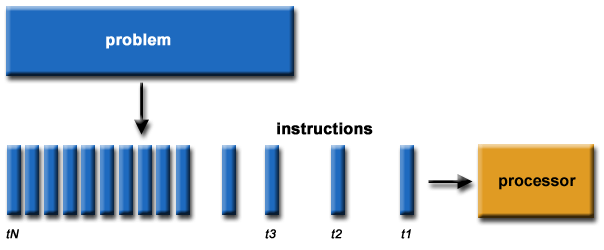
\includegraphics[width=\linewidth]{figs/serialProblem.png}
  \caption{Sequential processing where instructions (t1, t2, ..., tN) of a problem are executed by a single processors sequentially. \citep{Barney:16}}
  \label{fig:sequential-processing}
  \center
\end{figure}

\subsubsection{Parallel execution}
In parallel execution a problem can be broken into smaller sub-problems and two or more processors can work on it simultaneously. During this phase the processors may need to communicate with each other to exchange partial results. At the end of the computation the interim results from each processors must be combined to form the final solution to the original problem. Figure \ref{fig:parallel-processing} shows a problem is broken down into sub-problems each of which then consist of a set of instructions \textbf{(t1, t2, ..., tN)} that are executed by different processors in parallel.

\begin{figure}[!htb]
  \center
  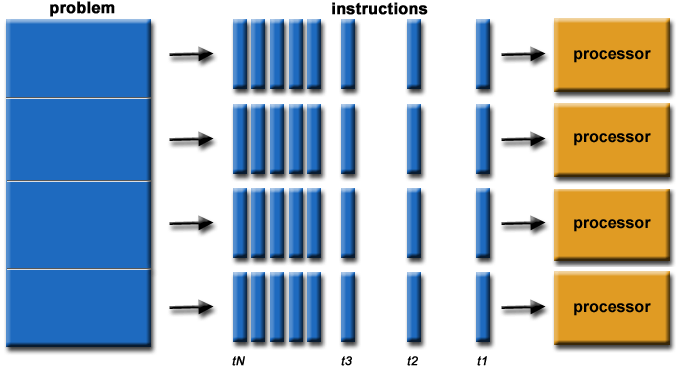
\includegraphics[width=\linewidth]{figs/parallelProblem.png}
  \caption{Parallel processing where a problem is broken down into a number of sub-problems with their own set of instructions (t1, t2, ..., tN) that can be executed in parallel by different processors. \citep{Barney:16}}
  \label{fig:parallel-processing}
  \center
\end{figure}

\subsection{Types of Parallelism}

\paragraph{Data parallelism}
In Data parallelism the input data is divided among different processors. The same task runs on different parts of the data in parallel. Data parallelism is a consequence of single operations that is being applied on multiple data items

\paragraph{Task Parallelism}
In Task parallelism different tasks run on the same data. In this model, parallelism is expressed by a task graph. A task graph can be either trivial or nontrivial. The correlation among the tasks are utilised to promote locality or to minimise interaction costs. This model is enforced to solve problems in which the quantity of data associated with the tasks is huge compared to the number of computation associated with them. The tasks are assigned to help improve the cost of data movement among different tasks.

\paragraph{Hybrid data/task parallelism}
A parallel pipeline of tasks, each of which might be data parallel

\subsection{Flynn's Classical Taxonomy}
This is known as one of the earliest classification of computers and programs created by Michael J. Flynn \citep{Barney:16}. Flynn classified programs and computers on instructions stream and data stream.

\begin{description}
\item [SISD] {Single Instruction Single Data}

Only one instruction is being acted on by the CPU during one clock cycle and only one data stream is being used as input.

\item [SIMD] Single Instruction Multiple Data

All processing unit execute same instruction at any given clock cycle but each processing using act upon different data input.

\item [MISD] Multiple Instructions Single Data

Each processing unit execute separate instruction stream independently on a single data stream.

\item [MIMD] Multiple Instructions Multiple Data

Each processor executes different instruction stream and all of them work on different data input stream.
\end{description}

This classification model distinguishes multi-processors computer architecture based on how they can be classified along the two independent dimension of Instruction Steam and Data Stream. There are further classification exist based on multiple data stream. \textbf{Single Program Multiple Data (SPMD)} is a subcategory of MIMD where multiple processors simultaneously execute same program on different data input.\citep{Barney:16}

\subsection{Classification of Parallel Computers}
Parallel computers can be classified based on their hardware supports. 
\begin{itemize}
	\item \textbf{PVP (Parallel Vector Processor)}

PVP systems contain a small number of powerful custom made vector processors with shared memory.
	\item \textbf{SMP   (Symmetric Multiprocessor)}
	
SMP system consist of a number of processors connected through a bus system. Each processor has equal access to memory, I/O etc.
	
	\item \textbf{MPP   (Massively Parallel Processor)}
	
MPP is very large-scale computer system with many processors and physically distributed memory space. This system requires high communication bandwidth and low latency interconnection between processors. It is a tightly couple system.
	
	\item \textbf{COW (Cluster of Workstation)}
	
COW is a low-cost variation of MPP which consist of multiple nodes(a complete workstation) connected by low-cost network. Nodes work together as a single integrated computing resource. This system is loosely coupled and highly extensible. Beowulf cluster falls into this category.
	
	\item \textbf{DSM  (Distributed Shared Memory)}
	
DSM uses special hardware and software extension to support distributed coherent caches. In contrast with SMP system, DSM consist of distributed-memory but hardware and software gives an illusion of shared-memory behaviour.
\end{itemize}
\citep{Perkowski:10}

\subsection{Parallel Computer Memory Architecture}
\paragraph{Shared Memory model}
Multiple processor operate independently but share the same address space. Figure \ref{fig:shared-memory} shows the shared-memory model architecture.

\begin{figure}[!h]
\centering
  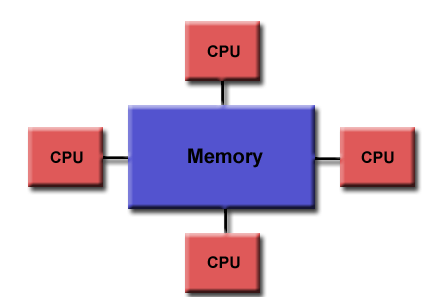
\includegraphics[width=.5\linewidth]{figs/shared-memory.png}
  \caption{A Shared Memory model where multiple CPU is sharing a common memory space. \citep{Barney:16}}
  \label{fig:shared-memory}
\end{figure}

\paragraph{Distributed Memory Model}
Processors have their own local address space. Memory address of one processor do not map to another. A message-passing mechanism is required for data sharing. Figure \ref{fig:distributed-memory} shows the distributed-memory model architecture.

\begin{figure}[!h]
\centering
  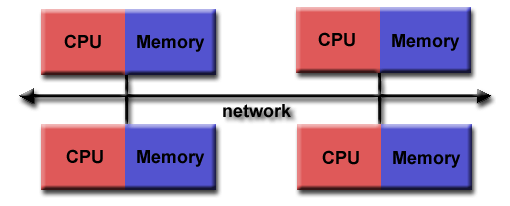
\includegraphics[width=.5\linewidth]{figs/distributed-memory.png}
  \caption{A Distributed Memory model where multiple CPUs have their own memory spaces but connected together with network bus to exchange messages. \citep{Barney:16}}
  \label{fig:distributed-memory}
\end{figure}

\paragraph{Hybrid Model}
Hybrid model is the combination of shared-memory interconnected by network communication that allows distributed-memory access of data resides in another processors global space. Figure \ref{fig:hybrid-memory} show the Hybrid-memory model architecture.

\begin{figure}[!h]
\centering
  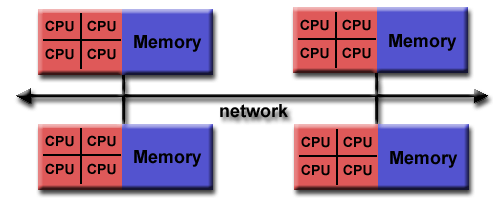
\includegraphics[width=.5\linewidth]{figs/hybrid-memory.png}
  \caption{A Hybrid Memory model where multiple shared-memory systems are interconnected together by a network communication  to exchange messages. \citep{Barney:16}}
  \label{fig:hybrid-memory}
\end{figure}

\citep{Barney:16}
\subsection{Limitation of Parallel Programming}
\subsubsection{Amdahl's Law}
Amdahl's law states that a programs speedup of an algorithm on parallel computing platform is defined by:

\[	S = \frac{1}{(1 - f) + \frac{f}{N}}  \]

Where,
\begin{itemize}
\item \textit{S} is the maximum speedup in execution time of entire task
\item \textit{f} is the percentage of the task that can be parallelise
\item \textit{N} is number of parallel processors 
\end{itemize}

From Amdahl's Law it become apparent that there is limits to the scalability of parallelism. The speedup gain on parallelising a tasks is dependent on the ratio of paralellisable codes \citep{Barney:16}. The graph in Figure \ref{fig:amdahls_law} shows the limit of speed up of parallel execution of code. This Law argued that there exist a  speed up limit; which is $ 1/(1-f) $.

\begin{figure}[!h]
\centering
  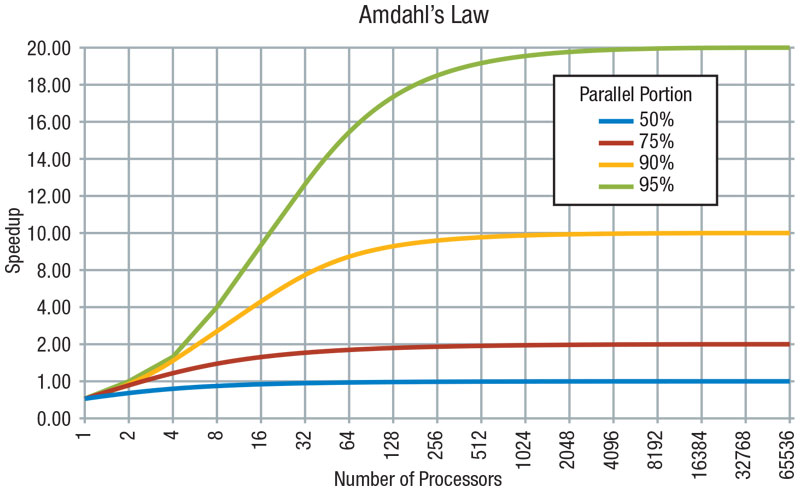
\includegraphics[width=.8\linewidth]{figs/amdahls_law.jpg}
  \caption{Amdahl's Law shows that speedup increases both as a function of the percentage of parallelism and the number of parallel units available. \citep{rtc_amdals:online}}
  \label{fig:amdahls_law}
\end{figure}

\subsubsection{Gustafson's Law}
The problem with Amdahl's law is that, it is assumed that the problem size is fixed for both serial and parallel parts. In an empirical studies by John Gustafson \citep{gustafson:88} showed that when problem size scales up, by scaling up the number of parallel processors the execution time can be kept fixed. The limitation imposed by the serial parts of a program may be countered by increasing the total amount of computation. This is known as Gustafson's law.

Gustafson's law is formulated as:

\[	S = (1 - f) + fN  \]
Where, 
\begin{itemize}
\item \textit{S} is the maximum speedup in execution time of entire task
\item \textit{f} is the percentage of the task that can be parallelise
\item \textit{N} is number of parallel processors 
\end{itemize}

In Figure \ref{fig:speed_up_fixed_scaled} the two models of parallel speedup contrasted and summarised in terms of gains based on fixed-size and scaled sized parallel portion in a program. As described by Amdahl's Law, if a program with \textit{s} serial portion and \textit{p}  parallel portion requires 1 time unit to run on a serial processors then it requires  $ s + p/N$ time unit on \textit{N} parallel processors. Therefor, the overall speed up is $ 1/(s+p/N)$. It is assumed that the parallel portion \textit{p} is fixed. 

In Figure \ref{fig:speedup_scaled} shows if the parallel portion of the program increases(where serial portion is shown as $ s' $ and parallel portion as $ p' $) time requires to run this program on serial processor is $ s' + Np'$ in comparison to running it on \textit{N} parallel processors. Therefore, if the number of processors \textit{N} is increased in proportion to the scaled up parallel portion of the program then the speedup is $ s' + Np'$.

\begin{figure}[!h]
	\begin{subfigure}[b]{\textwidth}
		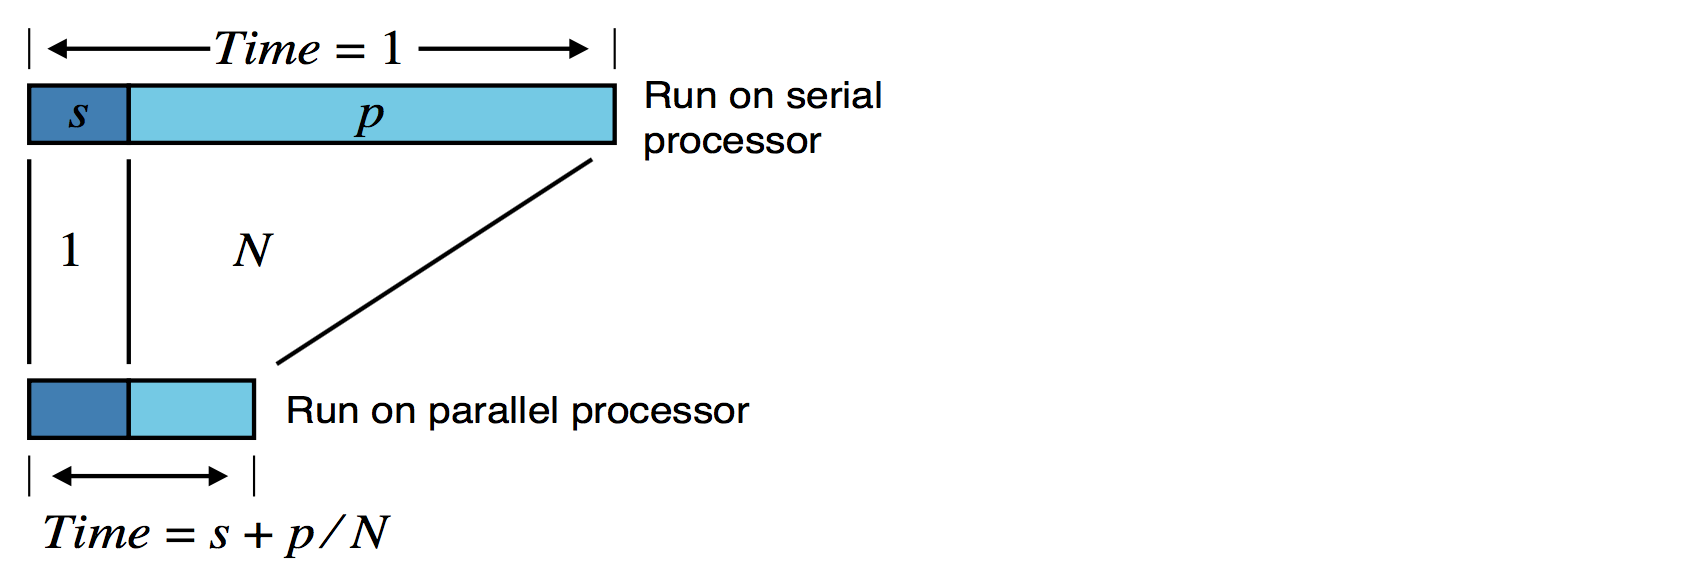
\includegraphics[width= .9 \textwidth]{figs/speedup_fixed.png}
  		\caption{A program with \textit{s} serial portion and parallel portion \textit{p} requires 1 time unit to run on a serial processors and  $ s + p/N$ on \textit{N} parallel processors. Therefor, the overall speed up is $ 1/(s+p/N)$.}
  		\label{fig:speedup_fixed}
	\end{subfigure}
	\begin{subfigure}[b]{\textwidth}
		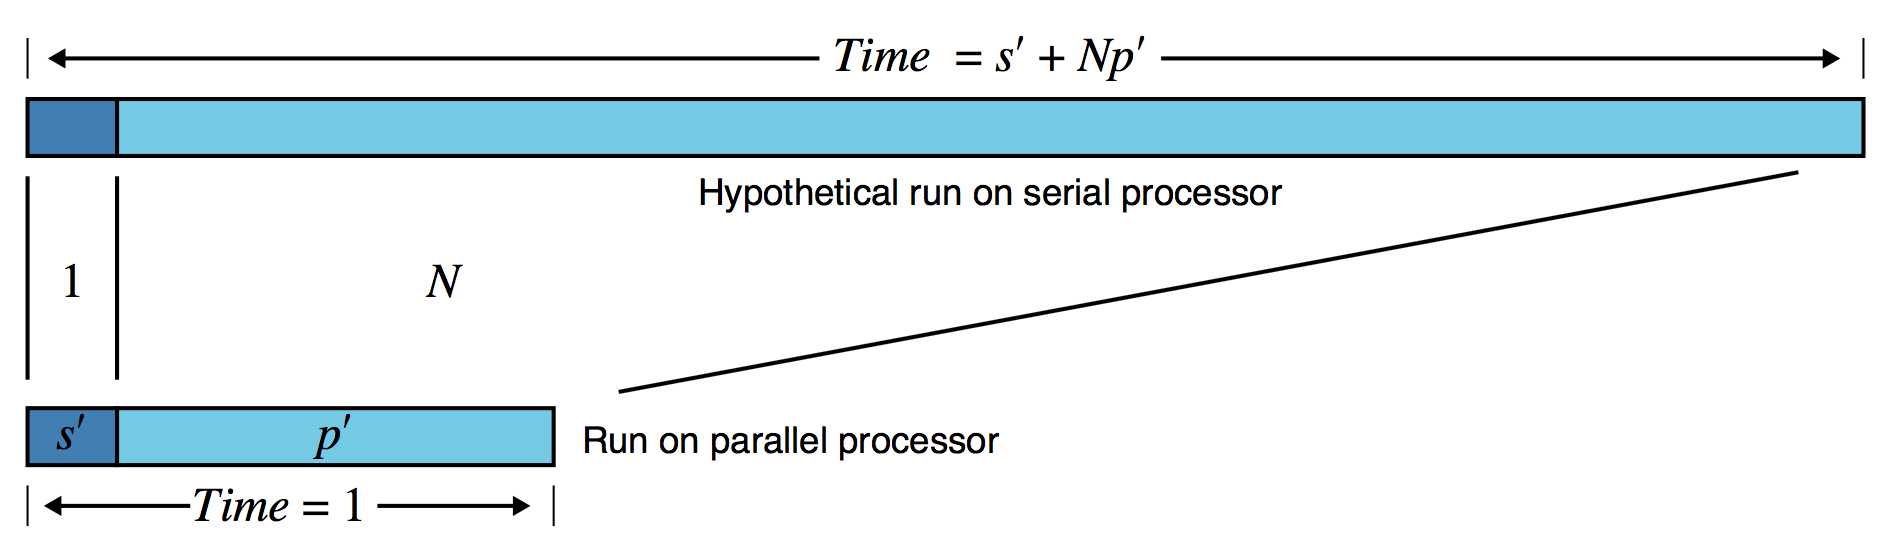
\includegraphics[width=\textwidth]{figs/speedup_scaled.png}
  		\caption{A program with $s'$ serial portion and $p'$ parallel portion requires 1 time unit to run on \textit{N} parallel processors and $ s' + Np'$ unit time on a serial processor. Therefor, the overall speed up is $ (s'+Np')/1$ i.e. $s'+Np'$.}
  		\label{fig:speedup_scaled}
	\end{subfigure}
	\caption{Comparison of speedup of fixed-sized and scaled-sizes parallel portion of a program.}
	\label{fig:speed_up_fixed_scaled}
\end{figure}

\citep{gustafson:88}

\subsection{Application}
Parallel computation many application areas, which include:
\begin{itemize}
	\item Scientific Computing
	\item Simulation
	\item Aerospace
	\item Weather forecasts - Climate changes
	\item Astronomy - Planetary movement
	\item Big Data and Data mining
\end{itemize}

\citep{Barney:16}

\section{OpenMP and MPI}
\subsection{OpenMP}
\label{openmp}
OpenMP stands for Open Multi-Processing. OpenMP is an Application Programming Interface (API) to facilitate parallel programming  on shared memory systems. \citep{chapman08}  It is a set of compiler directives and supporting callable runtime library routines and environment variables that extends C/C++ and Fortran to express shared memory parallelism. \citep{dagum:98}

In 1990's OpenMP was defined by OpenMP Architecture Review Board (ARB), formed by a group of leading Hardware and Software vendors to provide a common API for programming a range of SMP architectures. This was based on earlier similar work done by Parallel Computing Forum(PCF). Unlike MPI which we will discuss below, OpenMP is not a standard. Instead, it is considered as an agreement between members of ARB who shares common interest in portable, user-friendly and efficient approach to shared memory parallel programming. \citep{chapman08}
OpenMP API was designed to provide an easy method to thread application without requiring a programmer to know how to create threads, synchronise and destroy them or even how many to create.

OpenMP does not define a new language. It is a set of compiler directive that can be added to a sequential  program to describe how a work can be shared among threads executing on different processor cores and synchronise their access to shared data if needed. These compiler directives make it easy to modify a sequential program to take advantage of  shared-memory parallel architecture with a minimum modification to existing codes.
OpenMP is simple to use because the complexity of parallelism is handled by the compiler and also it emphasised on structured parallel programming. \citep{chapman08}

\subsubsection{Thread based parallelism}
OpenMP is based on Multithreading. Program launches as a single thread which can create other threads if required. It utilises the "fork" and "join" model of parallel execution.  All OpenMP program starts as a single process which is known as master thread. The master thread continues the program execution sequentially to the point where it encounter a parallel region of the program defined by a OpenMP construct directive. \citep{Barney:16-openmp}

\begin{figure}[!htb]
	\centering
	\begin{subfigure}[b]{\textwidth}
  		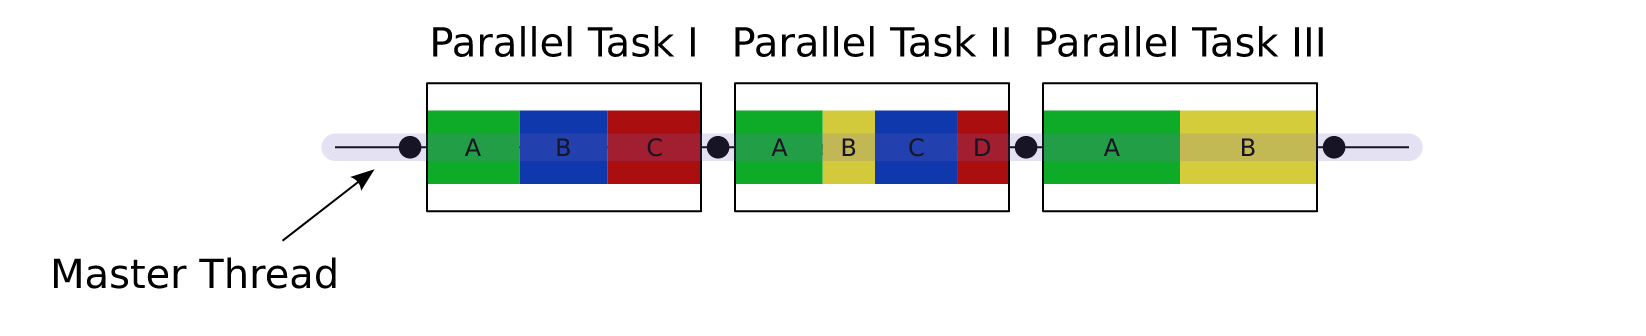
\includegraphics[width=\textwidth]{figs/fork_join_a.png}
  		\caption{Sequential execution: All of the Parallel Task blocks are executed by a single thread(Master).}
  		\label{fig:fork_join_a}
	\end{subfigure}
	\begin{subfigure}[b]{\textwidth}
  		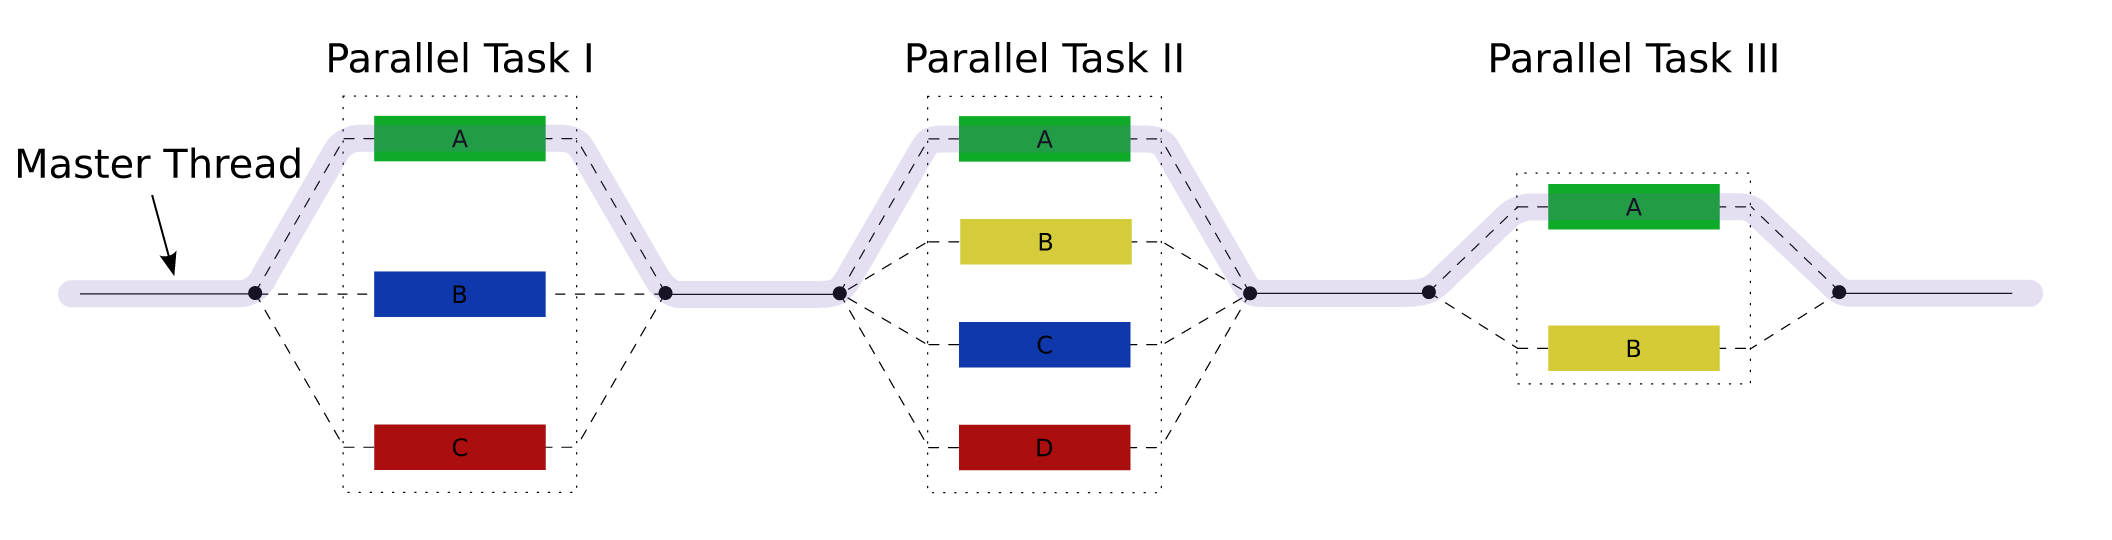
\includegraphics[width=\textwidth]{figs/fork_join_b.png}
  		\caption{Parallel execution: At each Parallel Task block the master thread forks multiple team threads which then execute the subtasks within that parallel region concurrently.  When finished the team threads then join with master thread and terminate before master thread advancing to the next parallel region.}
  		\label{fig:fork_join_b}
	\end{subfigure}
	\caption{Fork- Join model. \citep{A1:fork-join}}
  	\label{fig:fork-join}
\end{figure}

In Figure \ref{fig:fork-join} shows the fork-join model of parallel execution. It shows a program containing parallel executable code fragments. These code fragments are put into three region labelled as \textbf{Parallel Task I, Parallel Task II and Parallel Task III} to show the synchronisation points. Within these points program must synchronise before advancing. Each group contain code fragments of subtasks (labelled as A, B, C, D etc.) that are independent of each other and can be executed in parallel asynchronously. These subtasks can take advantage of concurrent execution by multiple threads. Figure \ref{fig:fork_join_a} shows the program is executed by a single thread(Master thread). The Figure \ref{fig:fork_join_b} shows that the same program is parallelise using fork-join model. When master thread reaches a parallel region it forks multiple team threads as required by that region. These team threads then execute the subtasks (A, B, C, D etc.) assigned to them concurrently. When the team threads complete executing the subtasks, they join back to the master thread and terminate. The master thread is then continue with rest of the program.

\subsubsection{OpenMP Components}
The OpenMP API comprised of three primary components:
\begin{itemize}
	\item Runtime Library Routines
	\item Environment Variables
	\item Compiler directives
\end{itemize}

\subsubsection{Runtime Library Routines}
The Runtime library routines are used for setting up  and identifying number of threads, thread numbers for identification, dynamically adjusting of threads, timers, nested parallelism and for locking mechanism. \citep{Barney:16-openmp}

\subsubsection{Environment Variables}
OpenMP provides several environment variables for controlling the execution of parallel code at runtime. These variables can be used to control the number of threads, scheduling type, binding threads to processor, controlling level of nested parallelism, dynamic thread adjustment, stack size and thread wait policy. \citep{Barney:16-openmp}


\subsubsection{Compiler Directives}
Compiler directives are special constructs that specify how a compiler should process its inputs. OpenMP API uses compiler directives for C, C++ and Fortran compilers for marking a parallel region, distributing works among threads, dividing up loop iterations, serialising section of codes and for synchronisation of the work. In C/C++ source code the directives appears as \#pragma as shown at Line 2 of Listing  \ref{lst:openmp_format}. \citep{Barney:16-openmp}

\begin{lstlisting}[language=C, caption={OpenMP directive format in C/C++}, label={lst:openmp_format}]

#pragma omp <directive-name> [clauses, ...] newline

\end{lstlisting}

Using OpenMP compiler directives a programmer instructs the compiler which part of program to run in parallel and how to divide the work among threads that  will run it. These directives are meaningful to the compilers only. OpenMP directives looks like comments in Fortran programs and pragma in C or C++ program. The advantage of such implementation is that a program containing OpenMP directives will still compile and run even if a compiler is unable to interpret these directives.

The line 5 in "Hello world" program showing in Listing \ref{lst:helloworld} is a compiler directive in C program that marks the region as a starting point of the parallel execution.

\begin{lstlisting}[language=C, caption={A "Hello world" program in C using OpenMP compiler directive}, label={lst:helloworld}]
#include <stdio.h>

int main(void)
{
    #pragma omp parallel
    printf("Hello, world.\n");
    return 0;
}
\end{lstlisting}

OpenMP directives can be classified in following categories:
\begin{itemize}
	\item Parallel region construct
	\item Work-sharing constructs
	\item Synchronisation constructs
	\item Data-scoped attribute clauses
\end{itemize}

\paragraph{Parallel region construct} A parallel region is a block of code that will be executed by multiple threads. This construct forks additional threads to carry out the work within the next parallel code block. Line 5 in Listing \ref{lst:helloworld} shows the parallel directive that specifies a parallel region \citep{Barney:16-openmp}

\paragraph{Work-sharing constructs}
A work-sharing construct specify how independent work to be assigned to one or more threads. The \emph{omp for} and \emph{omp do} is used to divide up loop iteration among multiple threads. The \emph{section} clause is for assigning non-iterative consecutive but independent code blocks to multiple threads. The \emph{single} clause specify that a code block is to be executed by only one single thread. A code block to be executed only by master thread the \emph{master} clause is used. Listing \ref{lst:openmp_for} shows an example of \emph{for} work-sharing construct. \citep{Barney:16-openmp}

\begin{lstlisting}[language=C, caption={An example of Work-sharing "for" loop construct.}, label={lst:openmp_for}]
 #include <omp.h>
 #define N 1000
 #define CHUNKSIZE 100

 main(int argc, char *argv[]) {
 int i, chunk;
 float a[N], b[N], c[N];

 /* Some initializations */
 for (i=0; i < N; i++)
   a[i] = b[i] = i * 1.0;
 chunk = CHUNKSIZE;
 #pragma omp parallel shared(a,b,c,chunk) private(i)
   {
   #pragma omp for schedule(dynamic,chunk) nowait
   for (i=0; i < N; i++)
     c[i] = a[i] + b[i];
   }   /* end of parallel region */ 
 }
\end{lstlisting}

\paragraph{Synchronisation constructs}
OpenMP provides synchronisation constructs to deal with race-condition to ensure that the correct results is produced. The synchronisation constructs are used to control how the execution of each thread progress in relation to other threads. The example in Listing \ref{lst:openmp_critical} shows the use of Critical directive to define a critical region a program. \citep{Barney:16-openmp}

\begin{lstlisting}[language=C, caption={An example of Critical directive construct.}, label={lst:openmp_critical}]
#include <omp.h>

main(int argc, char *argv[]) {
 int x;
 x = 0;
 
 #pragma omp parallel shared(x) 
   {
   #pragma omp critical 
   x = x + 1;
   }  /* end of parallel region */
}
 \end{lstlisting}

\paragraph{Data-scoped attribute clauses}
As OpenMP is shared-memory model of parallelisation, most variables are are shared among multiple threads. OpenMP provides number of clauses to deal with variable scopes to define their visibility. These clauses are used in conjunction with other directives to control the scope of enclosed variable within a parallel code block. \citep{Barney:16-openmp}

\subsubsection{Advantages \& Disadvantages of OpenMP}
\paragraph{Advantages}
The following are the advantages and disadvantages of OpenMP as discussed on Dartmouth  College website on parallel programming. \citep{Dartmouth:mpi}.
\begin{itemize}
	\item Good performance and scalability
	\item OpenMP programs are portable
	\item Easier to program and debug compared to MPI
	\item Allow program to be parallelised incrementally
\end{itemize}

\paragraph{Disdvantages}

\begin{itemize}
	\item Can only be run in Shared-memory computers
	\item Requires compiler that supports OpenMP
	\item Mostly used for loop parallelisation
\end{itemize}



\subsection{MPI}
\label{mpi}
MPI stands for \textbf{M}essage \textbf{P}assing \textbf{I}nterface. MPI is a standard specification for Message-Passing parallel programming model in distributed memory architecture. In Message-passing parallel model data is moved from one process's address space to another through cooperative message exchange. MPI itself is not a library but simply provides a standard specification for writing message passing programs. This standard defines the syntax and semantics of essential library routines that facilitates developers writing platform independent message-passing programs in C, C++ and Fortran. \citep{Barney:16-mpi}

MPI standard was a result of the works of many individuals and groups to address the problems they encounter in distributed memory model parallel programming. The need for an standard arose when a number of incompatible tools were developed independently by different groups. In 1992 a workshop on standards for Message-Passing in distributed memory environment was held sponsored by Center for Research on Parallel Computing, Williamsburg. This was followed by a draft proposal of MPI1 and forming of MPI Working group. The MPI1 draft proposal was presented in following year at Supercomputing 93 conference. MPI Working group held regular meetings, public comments and open mailing lists which later on constituted as \textbf{MPI Forum} \citep{Barney:16-mpi}. The current version of MPI standard is MPI 3.1 which was approved by MPI forum in June 2015. The next major version, MPI 4.0 is work in progress, which focuses on support on fault tolerance, improved support for hybrid programming models and application hints to MPI libraries to enable optimisations\citep{mpi-forum:16}.

\subsubsection{MPI Concepts}
The Message-passing approach makes data exchange cooperative between processes. Data is explicitly sent by one process and received by another. MPI is communication protocol and semantic specifications for how its features must behave in any implementation \citep{Gropp:99}.

To discuss various MPI constructs an example of matrix multiplication program using MPI is shown in Listing \ref{lst:mpi_example}. This code example is referenced in following subsections to explain some of these constructs.

\subsubsection{General MPI Program Structure}
Figure \ref{fig:mpi_structure} shows a general MPI program structure. MPI header files must be included by all programs that make MPI library call. MPI library calls are only permissible after initialising and before terminating the MPI environment\citep{Barney:16-mpi}. In the example program in Listing \ref{lst:mpi_example} line 28 initialises the MPI environment and line 111 terminates it.

\begin{figure}[!htb]
\begin{center}
  \includegraphics[width=.6 \linewidth]{figs/mpi_structure.png}
  \caption{MPI program structure}
  \label{fig:mpi_structure}
  \end{center}
\end{figure}

\subsubsection{Groups and Communicators}
MPI uses groups and communicators objects to define which process can communicate with each other \citep{Barney:16-mpi}. Processes can be collected into groups. Groups are implemented as ordered list of process identifiers stored in and integer array \citep{Gropp:96}. Each messages is sent in a context and must be received in the same context. A group and context together from a communicator \citep{Gropp:99}. \textbf{MPI\_COMM\_WORLD} is a predefined communicator that includes all MPI processes. Line 30 in Listing \ref{lst:mpi_example} shows that communicator \textbf{MPI\_COMM\_WORLD}  is used to query about number of available processes. 

\subsubsection{Rank}
In MPI  a process is identified by its \emph{rank} in the group associated with a communicator \citep{Gropp:99}. A \emph{rank} is a unique integer identifier. It is assigned by the system when a process is initialised. These identifies are contiguous and starts at '0'. The \emph{rank} id's are used by the programmers to specify the source and destination of messages \citep{Barney:16-mpi}.  Line 29 in Listing \ref{lst:mpi_example} shows that a process is querying its rank ID within the communicator \textbf{MPI\_COMM\_WORLD} .

\subsubsection{Error Handling}
The default action of an MPI call is to abort if there is a runtime error. However, most of the MPI function calls include a return/error code parameter. This allows a programmer to override the default behaviour of handling errors. \citep{Barney:16-mpi}

\subsubsection{Point-to-Point Communication}
Point-to-Point communication involves only two processes. One process performs send operation and other one performs receive operation. In MPI there are different types of send receives routines available such as:
\begin{itemize}
    \item \textbf{Synchronous send}
    
MPI\_Ssend() sends a message and blocks until the application buffer in the sending task is free for reuse and the destination process has started to receive the message.
    
    \item \textbf{Blocking send / blocking receive}
    
MPI\_Send()  is a basic blocking send operation. This routine returns only after the application buffer in the sending task is free for reuse. Similarly, MPI\_Recv() is a basic blocking receive operation that receive a message and block until the requested data is available in the application buffer in the receiving task.

    \item \textbf{Non-blocking send / non-blocking receive}
    
MPI\_Isend() is a non-blocking send operation that identifies an area in memory to serve as a send buffer. Processing continues immediately without waiting for the message to be copied out from the application buffer. A communication request handle is returned for handling the pending message status. Likewise, MPI\_Irecv()  is non-blocking  receive operation that identifies an area in memory to serve as a receive buffer. Processing continues immediately without actually waiting for the message to be received and copied into the the application buffer.

\end{itemize}
\citep{Barney:16-mpi}

Line 59 in Listing \ref{lst:mpi_example} shows an example of blocking send using MPI\_Send() routine my master process. There is a corresponding blocking receive call using MPI\_Recv() at line 107.

\begin{lstlisting}[language=C, caption={An example of Matrix multiplication using MPI. \citep{Barney:16-mpi}}, label={lst:mpi_example}]
include "mpi.h"
#include <stdio.h>
#include <stdlib.h>

#define NRA 62                 /* number of rows in matrix A */
#define NCA 15                 /* number of columns in matrix A */
#define NCB 7                  /* number of columns in matrix B */
#define MASTER 0               /* taskid of first task */
#define FROM_MASTER 1          /* setting a message type */
#define FROM_WORKER 2          /* setting a message type */

int main (int argc, char *argv[])
{
int	numtasks,  /* number of tasks in partition */
	taskid,			 /* a task identifier */
	numworkers,	 /* number of worker tasks */
	source,			 /* task id of message source */
	dest,				 /* task id of message destination */
	mtype,			 /* message type */
	rows,			   /* rows of matrix A sent to each worker */
	averow, extra, offset, /* used to determine rows sent to each worker */
	i, j, k, rc;           /* misc */
double	a[NRA][NCA],           /* matrix A to be multiplied */
	b[NCA][NCB],           /* matrix B to be multiplied */
	c[NRA][NCB];           /* result matrix C */
MPI_Status status;

MPI_Init(&argc,&argv);
MPI_Comm_rank(MPI_COMM_WORLD,&taskid);
MPI_Comm_size(MPI_COMM_WORLD,&numtasks);
if (numtasks < 2 ) {
  printf("Need at least two MPI tasks. Quitting...\n");
  MPI_Abort(MPI_COMM_WORLD, rc);
  exit(1);
  }
numworkers = numtasks-1;

/********** master task ************************/
   if (taskid == MASTER)
   {
      printf("mpi_mm has started with %d tasks.\n",numtasks);
      printf("Initializing arrays...\n");
      for (i=0; i<NRA; i++)
         for (j=0; j<NCA; j++)
            a[i][j]= i+j;
      for (i=0; i<NCA; i++)
         for (j=0; j<NCB; j++)
            b[i][j]= i*j;

      /* Send matrix data to the worker tasks */
      averow = NRA/numworkers;
      extra = NRA%numworkers;
      offset = 0;
      mtype = FROM_MASTER;
      for (dest=1; dest<=numworkers; dest++)
      {
         rows = (dest <= extra) ? averow+1 : averow;   	
         printf("Sending %d rows to task %d offset=%d\n",rows,dest,offset);
         MPI_Send(&offset, 1, MPI_INT, dest, mtype, MPI_COMM_WORLD);
         MPI_Send(&rows, 1, MPI_INT, dest, mtype, MPI_COMM_WORLD);
         MPI_Send(&a[offset][0], rows*NCA, MPI_DOUBLE, dest, mtype, MPI_COMM_WORLD);
         MPI_Send(&b, NCA*NCB, MPI_DOUBLE, dest, mtype, MPI_COMM_WORLD);
         offset = offset + rows;
      }

      /* Receive results from worker tasks */
      mtype = FROM_WORKER;
      for (i=1; i<=numworkers; i++)
      {
         source = i;
         MPI_Recv(&offset, 1, MPI_INT, source, mtype, MPI_COMM_WORLD, &status);
         MPI_Recv(&rows, 1, MPI_INT, source, mtype, MPI_COMM_WORLD, &status);
         MPI_Recv(&c[offset][0], rows*NCB, MPI_DOUBLE, source, mtype, MPI_COMM_WORLD, &status);
         printf("Received results from task %d\n",source);
      }

      /* Print results */
      printf("***************************\n");
      printf("Result Matrix:\n");
      for (i=0; i<NRA; i++)
      {
         printf("\n"); 
         for (j=0; j<NCB; j++) 
            printf("%6.2f   ", c[i][j]);
      }
      printf("\n***********************\n");
      printf ("Done.\n");
   }

/********** worker task ************************/
   if (taskid > MASTER)
   {
      mtype = FROM_MASTER;
      MPI_Recv(&offset, 1, MPI_INT, MASTER, mtype, MPI_COMM_WORLD, &status);
      MPI_Recv(&rows, 1, MPI_INT, MASTER, mtype, MPI_COMM_WORLD, &status);
      MPI_Recv(&a, rows*NCA, MPI_DOUBLE, MASTER, mtype, MPI_COMM_WORLD, &status);
      MPI_Recv(&b, NCA*NCB, MPI_DOUBLE, MASTER, mtype, MPI_COMM_WORLD, &status);

      for (k=0; k<NCB; k++)
         for (i=0; i<rows; i++)
         {
            c[i][k] = 0.0;
            for (j=0; j<NCA; j++)
               c[i][k] = c[i][k] + a[i][j] * b[j][k];
         }
      mtype = FROM_WORKER;
      MPI_Send(&offset, 1, MPI_INT, MASTER, mtype, MPI_COMM_WORLD);
      MPI_Send(&rows, 1, MPI_INT, MASTER, mtype, MPI_COMM_WORLD);
      MPI_Send(&c, rows*NCB, MPI_DOUBLE, MASTER, mtype, MPI_COMM_WORLD);
   }
   MPI_Finalize();
}
\end{lstlisting}

\subsubsection{Collectives Communication}
Collective Communication involves all processes in a process group. There are three types of Collective Communication routines:
\begin{description}
	\item \textbf{Synchornization}:
	These routines are used for process to wait until all members of the group have reached the synchronization point.
	\item \textbf{Data movement}:
	These type of routines are used to broadcast data to all processes, as well as scatter, gather or reduction of data to and from other processes.
	\item \textbf{Collective Computation}:
	These routines are use for one process of a communicator group to collect data from other members and perform operation on those.
\end{description}
\citep{Barney:16-mpi}

\subsubsection{Environment management}
MPI provides routines for managing execution environment to initialise and terminating MPI environment. The MPI environment is used to determine how many processes are participating in a computation and their rank within the group\citep{Gropp:96}. Environment management routines include querying rank identity as well as some other execution time related operations\citep{Barney:16-mpi}.

\subsubsection{Derived Data-types}
MPI predefines its primitive data types to achieve portability. This is because MPI supports heterogeneous environments(i.e different nodes) where the primitive types might have different representation\citep{mpi-forum:type-match}. Primitive data are contiguous. MPI also provides mechanism for user defined data structures based on sequence of these MPI primitive data types. Such data types are known as Derived data types and they are non-contiguous\citep{Barney:16-mpi}. An example of MPI derived datatype can been seen in Listing \ref{lst:pga_mpi_create_struct} which is an implementation parallel GA chromosome data structure.

\subsubsection{MPI advantages}
\begin{itemize}
	\item MPI provides a powerful, efficient and portable way to express parallel programs
	\item MPI is only Message-passing library that supports a standard, thus supported by almost any HPC platform
	\item There is little or no need for source code modification to port an application to a different platform that supports MPI standard
	\item Vendors can exploit native hardware features to improve performance on their own MPI implementation
	\item Popular MPI implementations are available both vendor and public domain
\end{itemize}
\citep{Barney:16-mpi}


\subsection{Hybrid Model}
MPI between nodes and Shared memory programming inside of each SMP(Symmetric Multiprocessing) node.


\section{Beowulf Clusters}
\label{bg/beowulf}
A Cluster is a independent group of computer nodes combined into an unified system through network and software systems that allows data to move between nodes\citep{Gropp:beowulf}.

There are two main usage of Cluster computing. One is performance and the other is fault-tolerance. Cluster computers can provide high performance through parallel computation. Such parallelism is achieve by coordinating many processors for single problem. Cluster computers can be used to address three main computational constraints: Realtime-constraints, Throughput and Memory limitation\citep{Gropp:beowulf}. The Cluster computing is dominating the HPC worldwide. The most recent[November, 2016] list of top performing Supercomputers shows that 86.4\% of the Top 500 Supercomputers are Clusters based \citep{Top500:cluster}. 

The Beowulf project defines Beowulf as scaleable performance clusters based on commodity hardware, on a private system network with open source software infrastructure\citep{Beowulf.org}. The main purpose of a Beowulf cluster is to achieve performance through parallel computations. This is accomplished by running programs across a number of nodes simultaneously and they may need to coordinate during program execution\citep{Gropp:beowulf}.

In 1994, first Beowulf cluster project was started as a experimental platform for parallel computing by Thomas Sterling, Donald Becker and their team at the NASA Goddard Space Flight center. Their aim was to build a low cost HPC(High Performance Computing) system for scientific computation with commodity hardware and open source software bundle. \citep{Gropp:beowulf}

\subsection{Architecture}
A Beowulf Cluster consists of one master node and one or more compute nodes connected by a System Area Network. Figure in \ref{fig:beowulf_arch} shows a basic Beowulf architecture. The compute nodes are connected through a private network. Master node can be connected to the external network if required\citep{Gropp:beowulf}. Beowulf differs from Cluster of Workstation(COW) for the fact that the entire system behave like a single machine. Only master node provides user interface. The compute nodes can be diskless or may contain small local storage. Jobs are initiated, scheduled and assigned by the master node.

\begin{figure}[!htb]
  \center
  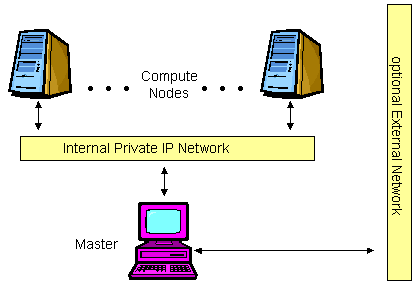
\includegraphics[width=.75 \linewidth]{figs/beowulf_arch.png}
  \caption{A basic Beowulf architecture. \citep{Beowulf:img}}
  \label{fig:beowulf_arch}
\end{figure}

\subsection{Hardware}
The main idea behind Beowulf project was to build HPC clusters using commodity hardware \citep{Gropp:beowulf}. The commodity hardware are those that are available Commercially-Off-The-Shelf (COTS) and not build for any specific purpose. These could be from PC-compatible hardware or rack-mounted servers to some embedded systems. The commodity status refers to the ability of obtaining such hardware on the open market and leveraging cheaper large scale productions. The biggest advantage of a Beowulf clusters is that it can be built with hardware produced by different vendors\citep{Thiru:05}

\subsection{Networking}
Beowulf clusters are group of individual machines that are meant to be interconnected to perform a task or number of tasks in parallel. In order to coordinate and complete execution efficiently the nodes in a cluster must be able to communicate with one another. Therefore, networks are very important components of a Beowulf cluster\citep{Gropp:beowulf}.

A Beowulf cluster with small number of nodes commodity networking technologies like Gigabit Ethernet are widely used. However, as the number of nodes increases network latency becomes a bottleneck for overall cluster performance. To overcome this, different network topology such hypercube topology and high-end networking hardware are used\citep{Thiru:05}.

\subsection{Software Infrastructure}
\paragraph{Operating Systems}
Linux is widely used on Beowulf clusters because it is open source, reliable and cost free. Another alternative is FreeBSD which is also open source. Open source nature of these Operating Systems are attractive to Beowulf community as it allows the kernel to be customised for specific needs and setup. \citep{Gropp:beowulf}

\paragraph{Middleware}
Coordination and communication between the processing nodes in cluster is key requirement. Beowulf utilises Message-passing model of parallel architecture. Both MPI and PVM(Parallel Virtual Machine) API can be deployed in a Beowulf systems. However, having a standard API and wider portability MPI become a popular choice for parallel programming in Beowulf. \citep{Gropp:beowulf}

\paragraph{Job control}
The Operating System only manages local jobs by itself. In distributed memory model additional job controller software is required. This job control program responsible for system partitioning, queuing jobs, how jobs start and run on remote nodes\citep{Gropp:beowulf}. Example of such parallel job control systems are PBS(Portable Batch System), Hydra and MPD. 

\section{Simple Genetic Algorithm (SGA)}
\label{sga}
In his renowned book on Genetic Algorithm David E. Goldberg \citep{Goldberg:89} describes Genetic Algorithms(GA) as search and optimisation technique which is based on the theory of natural selections and natural genetics. These are general search and optimisation algorithms that use the theories behind the evolution as a tool to find optimal or near optimal solution to difficult problems. This involves evolving a population of possible solutions to the particular problem by using operations inspired by natural genetic variation and natural selection \citep{Murphy:03}. 
It simulates the "survival of the fittest" among individual solution over consecutive generation for solving a problem. In 1960's Genetic Algorithms were pioneered by John Holland along with his colleagues and students at University of Michigan\citep{Murphy:03}.

\subsubsection{Optimisation using GA}
In science and Engineering there exist many problems that have solution space too large or sometimes even an infinite set. In those case it is impossible to check each individual solution and try to find the best one. One approach to finding a solution of such problems is limiting the number of possibilities and range with a given step size for lookup. The set of possible solution are known as 'search space'. 

Each possible solution can be marked by its value of fitness for the problem.  Using this fitness value, the algorithm determines which set of solutions are going to forward to produce new solutions. GA attempt to find the best solution based on its fitness value to a given problem. This is achieved by using a combination of \emph{exploitation} and \emph{exploration}. When the algorithm has found a number of good possible solutions it exploits them by combining different parts of each solution to form a new candidate solutions. This is known as \emph{crossover}. GA also do some experiment by creating new candidate solutions by randomly changing parts of old solutions which is known as \emph{mutation}. \citep{Murphy:03}.

In his Master thesis Roderick Murphy described GA as 'weak' optimisation of searching procedure as they do not use any domain specific knowledge to do so\citep{Murphy:03}. Instead GA utilise some 'random' choice to guide its search by exploiting historical information to direct the search into a region of optima.
\subsubsection{GA terminology}
\paragraph{Population:}
Population is a subset of all possible solutions to the given problem.
\paragraph{Chromosome:}
A chromosome is one individual solution to the problem.
\paragraph{Gene:}
A gene is one element position of a chromosome.
\paragraph{Allele:}
Allele is the particular value of a gene in a chromosome.
\paragraph{Locus:}
The position of a gene on the chromosome.
\paragraph{Genotype:}
Genotype is the population in the computation space.
\paragraph{Phenotype:}
Phenotype is the population in the real world solution space.
\citep{Murphy:03}
 
\subsubsection{Computer Implementation}
To utilise GA one must encode solutions to a problem in a structure that can be stored in the computer. A solution to a problem is represented as  string known as \emph{chromosome}(strings) that consist of a combination of several genes(simple representation are binary 1's \& 0's). If we consider a multi-variable problem, a gene can be considered as the bits that encode a particular parameter and its allowable value. A set of solutions to the problem is represented by a group of chromosomes referred to as a \emph{population}. During each iteration of the algorithm the chromosomes in the population will undergo one or more genetic operations such as \emph{crossover} and \emph{mutation}. The result of the genetic operations will become the next generations of the population. This process continues until a solution is found or a certain termination condition is met. \citep{Murphy:03}

\subsubsection{Genetic Operators}
Genetic Operators are responsible for altering the genetic composition of offspring. There three operators:
\begin{itemize}
	\item Selection
	\item Crossover
	\item Mutation
\end{itemize}

\subsubsection{Selection}
Selection operator is used for selecting candidate solutions for reproduction. The probability of selection should be proportional to the fitness value of the chromosome itself. The selection process is very important for maintaining good diversity and preventing premature convergence. There are several methods of how to select the best chromosomes. 

\paragraph{Roulette wheel selection:} In roulette wheel selection parents are selected according to their fitness. The better the fitness value the higher the chances to be selected.
\paragraph{Rank selection:} Rank selection first ranks the population and then every chromosome receives fitness from this ranking. In population with N chromosome, the worst chromosome will have rank 1, second worst  will have 2 and the best one will have N.
\paragraph{Tournament selection:} In Tournament selection K number of individuals are taken from the population then select the best out of these using their fitness value. The process is repeated for selecting next parent.
\citep{tutp.com:98ga}

\subsubsection{Crossover}
The primary purpose of crossover operator is to get genetic material from the previous generation to the next generation. This is done by selecting two parents and then exchanging some parts of their genes. This produces two new offsprings. There are different ways of exchanging genes.
\paragraph{Single-point crossover}
This is the simplest form of crossover in which a random crossover point is selected and the bits from this point get swapped with between two parents to get new offsprings. Figure \ref{fig:sp-cross} demonstrate the the single-point crossover.

\begin{figure}[!htb]
  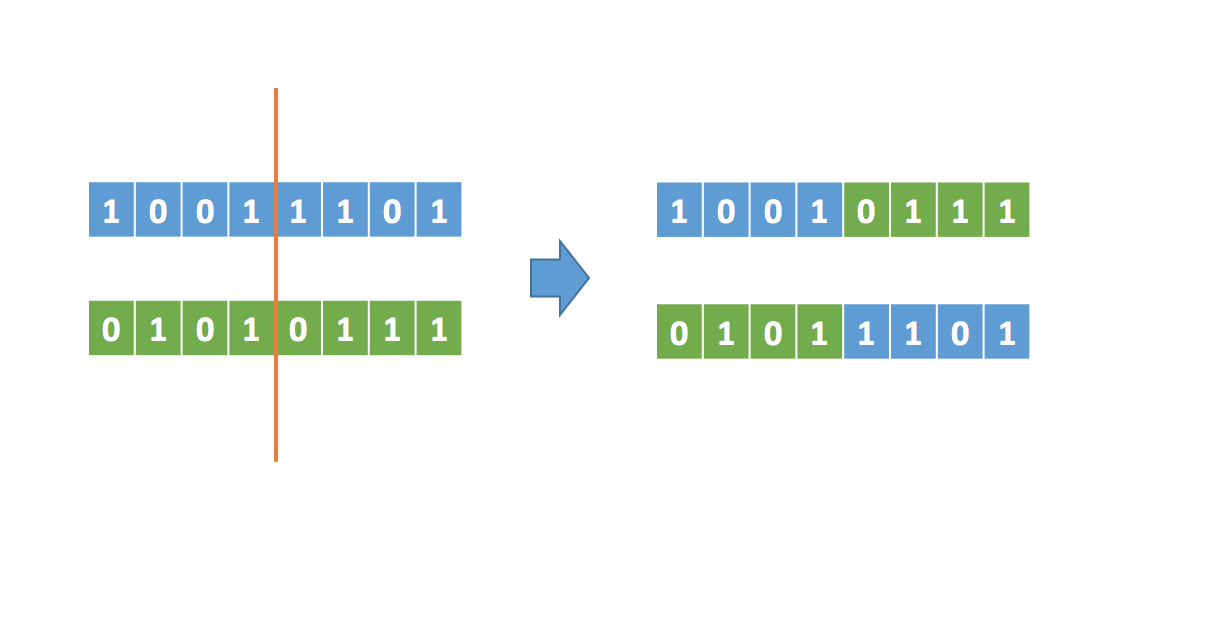
\includegraphics[width=\linewidth]{figs/single-point_crossover.png}
  \caption{Single-point crossover}
  \label{fig:sp-cross}
\end{figure}

\paragraph{Multipoint crossover}
In mulit-point crossover a number of crossover points are chosen and then bits segments in every second group are swapped between two parents to produce new offsprings. Figure \ref{fig:mp-cross} shows multi-point crossover. 

\begin{figure}[!htb]
  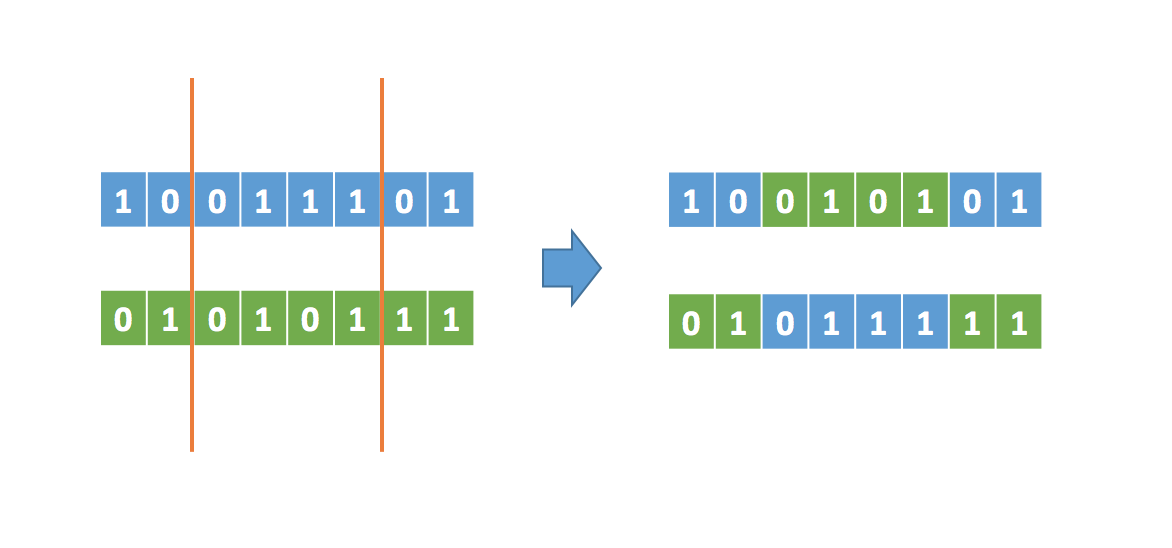
\includegraphics[width=\linewidth]{figs/multi-point_crossover.png}
  \caption{Multi-point crossover}
  \label{fig:mp-cross}
\end{figure}

\paragraph{Uniform crossover}
Uniform crossover is a variation of multi-point crossover. In this method random decision is made whether a bit groups will be swapped or not between two parents to produce new offsprings. Figure \ref{fig:uniform-cross} shows uniform crossover. 

\begin{figure}[!htb]
  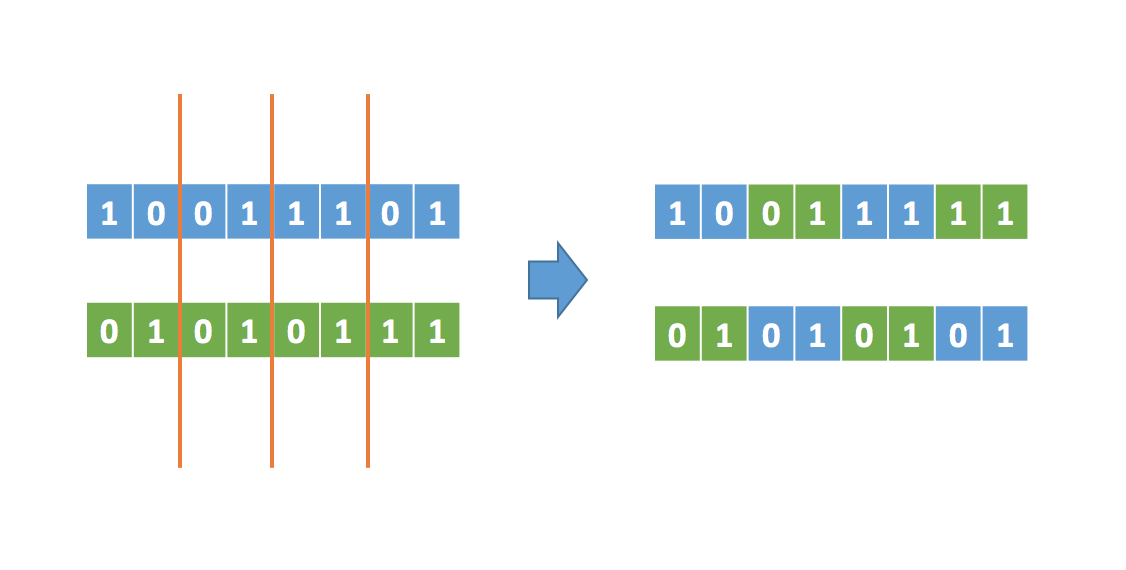
\includegraphics[width=\linewidth]{figs/uniform_crossover.png}
  \caption{Uniform crossover}
  \label{fig:uniform-cross}
\end{figure}
\citep{Murphy:03}

\subsubsection{Mutation}
Mutation operator create new offspring by making small tweak in chromosome. It can help creating chromosomes that would not otherwise be formed by applying selection and crossover operators alone. Mutation can allows GA to explore the search space and keep it from getting trapped in a local optimal solutions. There are several methods of mutation such as bit flipping, random resetting, swap mutation and inversion mutation\citep{tutp.com:98ga}. Figure \ref{fig:mutation} shows bit flipping and Swap mutation.

\begin{figure}[!htb]
  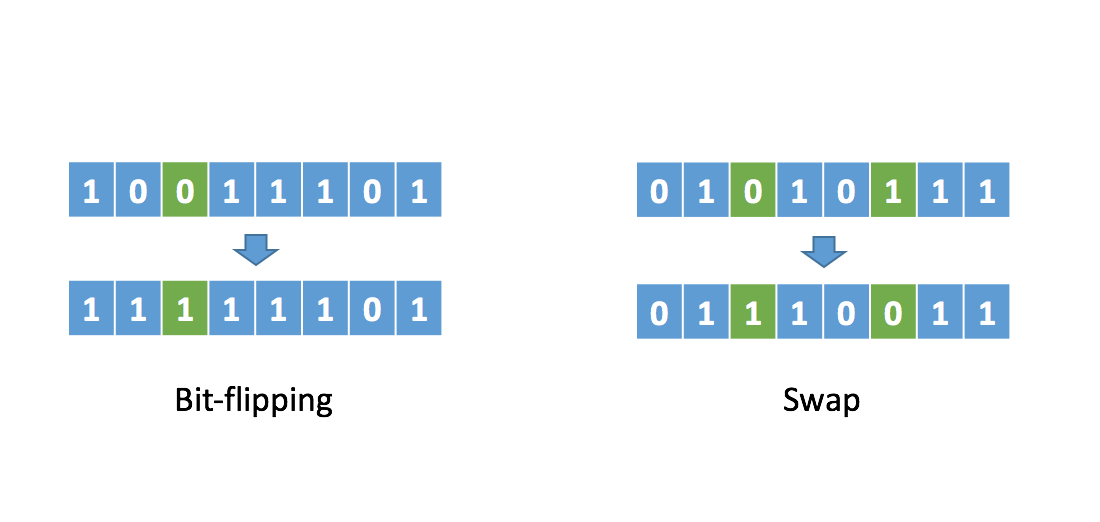
\includegraphics[width=\linewidth]{figs/mutation.png}
  \caption{Mutation}
  \label{fig:mutation}
\end{figure}

\subsubsection{Simple Genetic Algorithm}
\begin{enumerate}
\item \textbf{Start:} Generate random population of n chromosomes (suitable solutions for the problem)
\item \textbf{Fitness:} Evaluate the fitness f(x) of each chromosome x in the population
\item \textbf{New population:} Create a new population by repeating following steps until the new population is complete
	\begin{enumerate}
	\item \textbf{Selection:} Select two parent chromosomes from a population according to their fitness (the better fitness, the bigger chance to be selected)
	\item \textbf{Crossover:} With a crossover probability cross over the parents to form a new offspring (children). If no crossover was performed, offspring is an exact copy of parents.
	\item \textbf{Mutation:} With a mutation probability mutate new offspring at each locus (position in chromosome).
	\item \textbf{Accepting:} Place new offspring in a new population
	\end{enumerate}
\item \textbf{Replace:} Use new generated population for a further run of algorithm
\item \textbf{Test:} If the end condition is satisfied, stop, and return the best solution in current population
\item \textbf{Loop:} Go to step 2
\end{enumerate}
\citep{Obitko:98}

\subsubsection{Application of GA}
Genetics Algorithms are very effective way of quickly finding a reasonable solution to a complex problem. GAs are most effective in search space for which little is known. Apart from general optimisation problems, Genetic Algorithms are successfully deployed on diverse range of other fields. These include tasks optimising, dynamic programming, machine learning, economics, immune systems, ecology, population genetics and social systems. \citep{Murphy:03}


A more recent development is the use of Evolutionary Computation (EC) to evolve the control structures for humanoid robotics \citep{eaton2015}. Writing software in a traditional manner to controls the very large number of articulation points is beyond the capability of a human programmer \citep{eaton2015}. Techniques that leverage GAs have been demonstrated to effectively equip humanoid robotic platforms with abilities to simulate the mechanics of incredibly complex human movement such as kicking a soccer ball.

\subsubsection{Advantages}
Genetic Algorithms have many advantages which inlcude:
\begin{itemize}
\item Does not require any derivative information (which may not be available for many real-world problems).
\item Is faster and more efficient as compared to the traditional methods.
\item Has very good parallel capabilities.
\item Optimizes both continuous and discrete functions and also multi-objective problems.
\item Provides a list of "good" solutions and not just a single solution.
\item Always gets an answer to the problem, which gets better over the time.
\item Useful when the search space is very large and there are a large number of parameters involved.
\end{itemize}

\subsubsection{Limitations}
There are number limitation with Genetic Algorithms that we must consider. These include:
\begin{itemize}
\item GAs are not suited for all problems, especially problems which are simple and for which derivative information is available.

\item Fitness value is calculated repeatedly which might be computationally expensive for some problems.

\item Being stochastic, there are no guarantees on the optimality or the quality of the solution.

\item If not implemented properly, the GA may not converge to the optimal solution
\end{itemize}

\citep{pit:95}



\section{Parallel GA}
\section{Parallelising Procedural GA using MPI}
\subsection{Parallel GA model}
The master-slave model of parallel GA is adopted for this implementation. The operation most commonly parallelised in master-slave model is the evaluation of the fitness function as in general this requires only individuals values not the entire population so that the communication is minimum between nodes. Parallelising the evaluation of fitness function is done by assigning a part of population to each node available in a cluster. Message passing occurs when slave nodes receive the subset of global population and returns evaluated fitness values to the master. 

Figure \ref{fig:flowchart_pga} represent the flowchart of implemented Parallel GA. Dotted line shows Message passing communication between Master and Slaves. This flowchart shows the diagram of implemented parallel GA using the procedural SGA discussed earlier in this section. As we can see from this diagram Master process responsible for initialising first generation of population, evaluate and report on them. The next task for the master process is to dividing up population among available slave processes. 

\begin{figure}[!hp]
    \vspace*{-1cm}
    \makebox[\linewidth]{
        \includegraphics[width=.9 \linewidth]{figs/flowchart_pga2.png}
    }
    \caption{Flowchart diagram of Implemented master-slave Parallel GA}
     \label{fig:flowchart_pga}
\end{figure}


The following subsections explain various MPI directives implemented.

\subsection{Initialising MPI environment}
As with all MPI program the message-passing environment needs to be initialised prior to calling any message-passing procedure. This is done by calling MPI\_Init() procedure on line 8 shown in the code fragments on Listing \ref{lst:pga_initialise_mpi}. MPI uses objects known as communicators and groups to define which collection of processes may communicate with each other. MPI\_Comm\_size() returns number of processes available for MPI communication and MPI\_Comm\_rank() returns its own unique rank id for identification within a communicator group.

\begin{lstlisting}[language=C, caption={Parallel GA implementation using MPI: Source code of main()}, label={lst:pga_initialise_mpi}]
MPI_Init(&argc, &argv);
MPI_Comm_size(MPI_COMM_WORLD, &numNodes); // How many nodes
MPI_Comm_rank(MPI_COMM_WORLD, &myId); // My Rank ID
\end{lstlisting}

\subsection{Creating MPI derived datatype for genotype}
MPI requires data to be in a contiguous memory location for marshalling and demarshalling of data to send and receive. Any non-primitive datatype needs to be defined for MPI to handle this properly. Listing \ref{lst:pga_mpi_create_struct} shows the procedure for creating a MPI derived datatype for the genotype struct of SGA. Line 14 contains the MPI routine MPI\_Type\_create\_struct() that requires 3 arrays containing information about user data types, their count and their offsets values within the struct along with original data type that is being converted and an MPI\_Datatype object where this routine will return the new type on success. In lines 7-12 the offsets values of genotype members are being stored in offsets array using C library macro offsetof() function.

\begin{lstlisting}[language=C, caption={Creating an MPI derived data type for genotype struct.}, label={lst:pga_mpi_create_struct}]
void create_mpi_genotype_struct(MPI_Datatype& mpi_genotype){
    const int nitems = 6;
    int blocklengths[6] = {NVARS, 1, NVARS, NVARS, 1, 1};
    MPI_Datatype types[6] = {MPI_DOUBLE, MPI_DOUBLE, MPI_DOUBLE, MPI_DOUBLE, MPI_DOUBLE, MPI_DOUBLE};
    
    MPI_Aint     offsets[6];
    offsets[0] = offsetof(genotype, gene);
    offsets[1] = offsetof(genotype, fitness);
    offsets[2] = offsetof(genotype, upper);
    offsets[3] = offsetof(genotype, lower);
    offsets[4] = offsetof(genotype, rfitness);
    offsets[5] = offsetof(genotype, cfitness);
    
    MPI_Type_create_struct(nitems, blocklengths, offsets, types, &mpi_genotype);
    MPI_Type_commit(&mpi_genotype);
}
\end{lstlisting}


\subsection{Partitioning of data}
Following strategy shown in Listing \ref{lst:pga_partitioning} is applied to partition the population among available nodes. A 2D array node\_data[][] shown in line 1 is used to hold the starting index and the row count for a given node id. From line 3 to line 11 the starting index and row counts are calculated and stored in node\_data[][] array for each node\_id. 

\begin{lstlisting}[language=C, caption={Partitioning population data among nodes}, label={lst:pga_partitioning}]
    int nodes_data[numNodes][2]; // Array to hold data partition information
    int start_i, num_rows;
    int chunk_size = (int)(ceil((double) POPSIZE / numNodes));
               
    for(int i = 0; i < numNodes; i++)
    {
        start_i = i * chunk_size;
        num_rows = min(chunk_size, POPSIZE - start_i);
        nodes_data[i][0] = start_i;
        nodes_data[i][1] = num_rows;
    }
\end{lstlisting}

\subsection{PGA v1}

\subsubsection{Master-Slave Communication}
In master-slave model all processes run the same MPI program. But depending on its role each process executes parts of the program. The parts of the main() shown in Listing \ref{lst:pga_mpi_main}. On line 3 each process gets its own communicator ID by calling MPI\_Comm\_rank(). Using this ID master process executes the master\_process() (line 5) and all other process executes slave\_process()(line 9). 

\begin{figure}[!htb]
        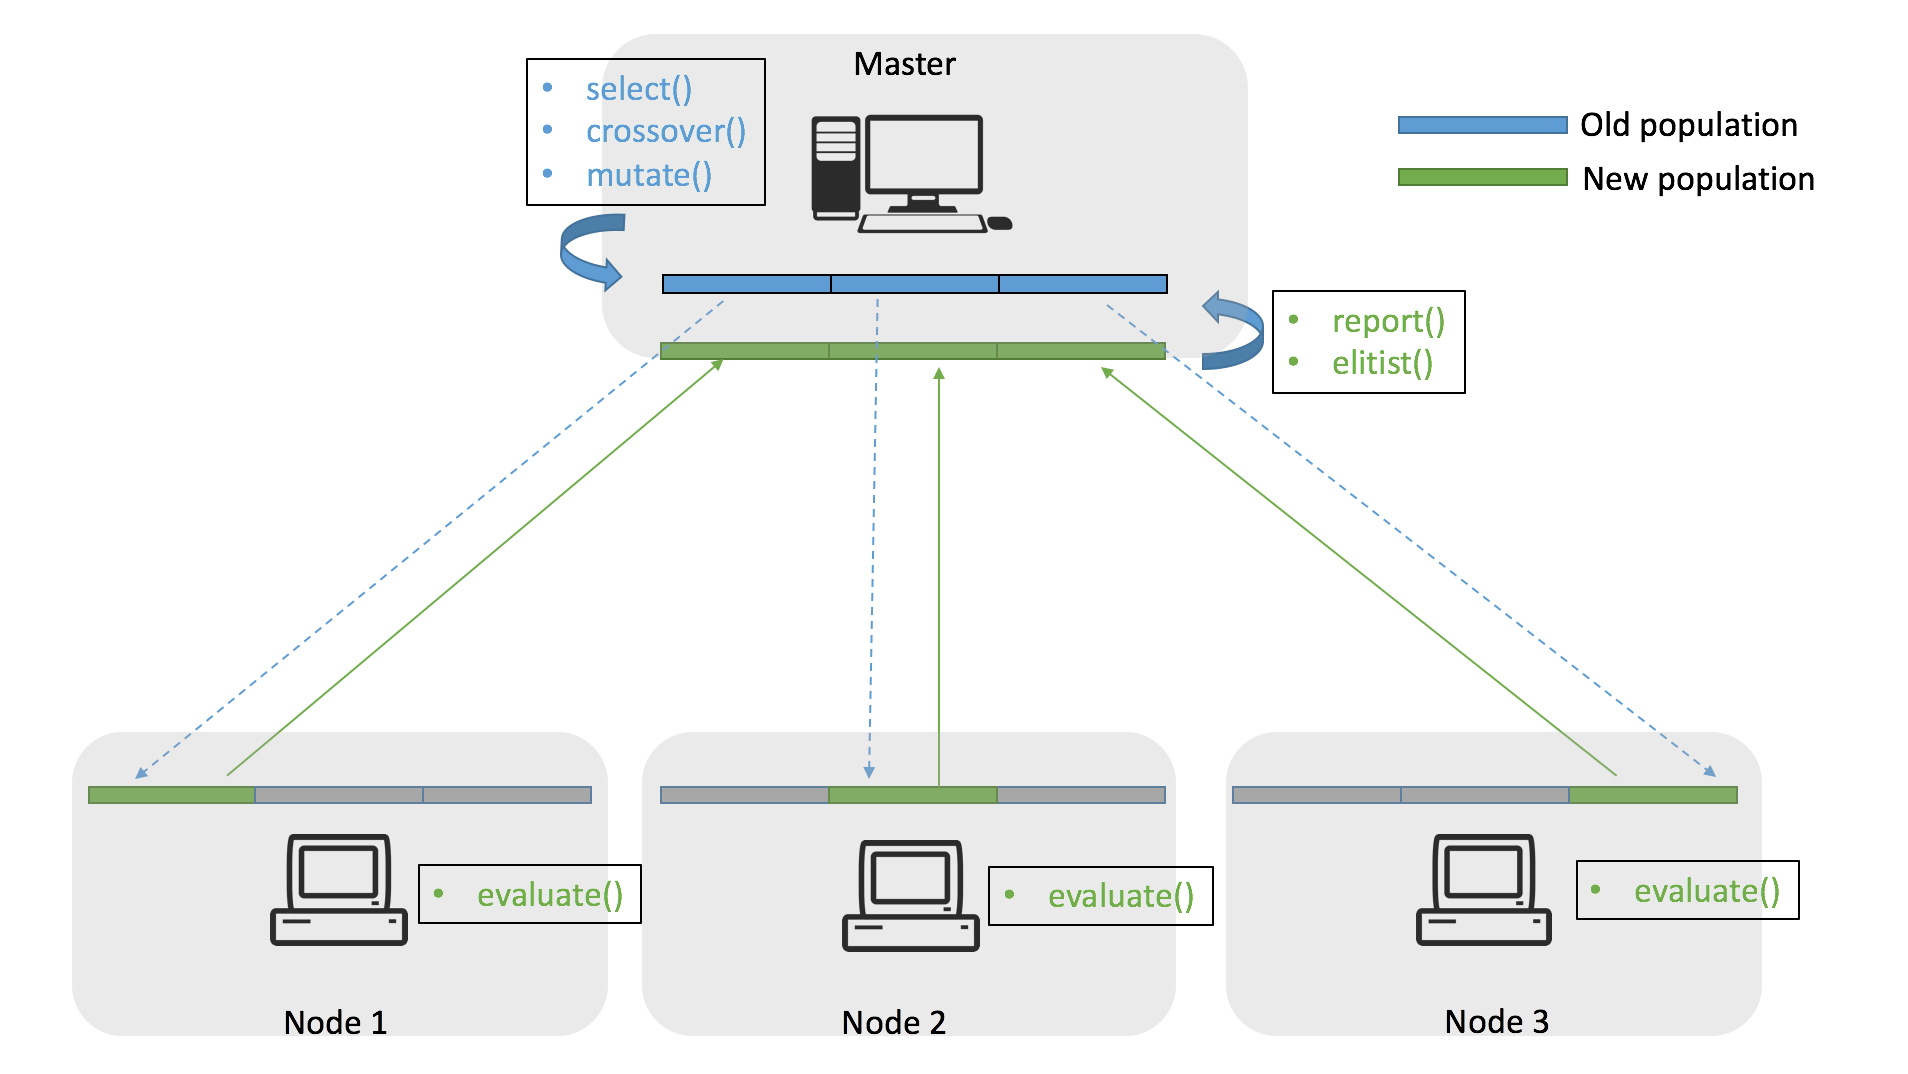
\includegraphics[width= \linewidth]{figs/pga_model_v1.png}
    \caption{PGA v1 model}
     \label{fig:pga_model_v1}
\end{figure}

For each generation, the master\_process() is responsible for performing selection, crossover and mutation operation on entire population ,  dividing population among all available nodes, updating all nodes with their parts of current population, collecting evaluated fitness values from each nodes, evaluate the best member for that generation, report and perform elitist operation on entire population. Where slave process is only responsible to receive a subset of population from master, evaluate their fitness values, send them back to master.  Figure \ref{fig:pga_model_v1} shows the master and slave data decomposition and the GA operation they perform on the population data depends on their role.

\begin{lstlisting}[language=C, caption={Master and slave pr}, label={lst:pga_mpi_main}]
ierr = MPI_Init(&argc, &argv);
ierr = MPI_Comm_size(MPI_COMM_WORLD, &numNodes); // How many nodes
ierr = MPI_Comm_rank(MPI_COMM_WORLD, &myId); // My Rank ID
    
if(myId == MASTER_ID) // Master Process
{
      master_process(filename, seed, mpi_genotype, nodes_data, start);
}
else // Slave processes
{  
    slave_process(seed, mpi_genotype, nodes_data);
}
\end{lstlisting}

\subsubsection{Master process}
In Listing \ref{lst:pga_master_process} parts of the master\_process() procedure is shown. After initialising the initial population master starts performing GA operation on them(lines 3-6). On lines 9-14 it starts sending subset of population to each nodes using MPI\_Send() routine. As we shall see in Listing \ref{lst:pga_slave_process} there is a corresponding MPI\_Recv routine call (line 2) invoked by the slave process. Master then evaluate it's own parts the population subset (line 17). On lines 20-25 master starts to gather the parts of population which have their fitness value calculated by the slave nodes. Then on line 27 master perform elitist() operation using entire population.

\begin{lstlisting}[language=C, caption={The master\_process() procedure.}, label={lst:pga_master_process}]
for(int generation = 0; generation < MAXGENS; generation++)
{   
      selector ( seed );
      crossover ( seed );
      mutate ( seed );     
      report(generation);

      int start_index, item_count;
      for(int nodeId = 1; nodeId < numNodes; nodeId++)
      {
          start_index = nodes_data[nodeId][0];
          item_count = nodes_data[nodeId][1];
          MPI_Send(&population[start_index], item_count, mpi_genotype, nodeId, SEND_DATA_TAG, MPI_COMM_WORLD);
        }
        
      /* Evaluate master's parts of the population */
      evaluate(nodes_data[0][0], nodes_data[0][1]);
        
      /* Collect all parts of new population from each node */
      for(int nodeId = 1; nodeId < numNodes; nodeId++)
      {
          start_index = nodes_data[nodeId][0];
          item_count = nodes_data[nodeId][1];
          MPI_Recv(&population[start_index], item_count, mpi_genotype, nodeId, RETN_DATA_TAG, MPI_COMM_WORLD, &status);
       }
                
      elitist();
}
\end{lstlisting}

\subsubsection{Slave process}
As we can see in Listing \ref{lst:pga_slave_process} the slave process starts with a MPI\_Recv() call on line 4. After receiving the parts for the population slave process perform evaluate() using its own starting index and row count on line 7. When the fitness evaluation is done it start to send the population part to master process by calling MPI\_Send() routine.


\begin{lstlisting}[language=C, caption={The slave\_process() procedure.}, label={lst:pga_slave_process}]
for(int generation = 0; generation < MAXGENS; generation++)
{
    /* Get a subset of population from master */
    ierr = MPI_Recv(&population[my_start], row_count, mpi_genotype, MASTER_ID, SEND_DATA_TAG, MPI_COMM_WORLD, &status);
        
    /* Perform fitness evaluation */
    evaluate (my_start, row_count);
        
    /* Send evaluated population to master */
    MPI_Send(&population[my_start], row_count, mpi_genotype, MASTER_ID, RETN_DATA_TAG, MPI_COMM_WORLD);
}
\end{lstlisting}


\subsection{PGA v2}
\subsubsection{Performance issue with PGA v1}
The first implementation of Master-slave GA as in PGA v1 distribute evaluation of fitness function among several slave processors while master executes the GA operations(selection, crossover and mutation). This implementation explore the search space in exactly same manner as a serial GA and follows exactly the same simple GA design guidelines. It is thought to be the case that, this implementation of master-slave parallel GA results in significant improvement in performance. However, as we shall see in Chapter \ref{empirical} when empirical studies were carried out the actual performance gains seemed to be worse than the serial GA. This is perhaps for the frequent MPI communication overhead that required in each generation for evaluating fitness values back and forth to the master and slave nodes. The execution time time of master-slave GAs have two components; the time used for communication between nodes and the time used in computation. So, the other reason is, master is responsible for performing all GA operations on entire population while slave nodes are mostly sitting idle during this time. With this approach slave nodes are under utilised where master node has a lot of workload 

So, in this version of PGA we tried to leverage some of the GA operations as well as evaluating fitness values to the slave nodes. The movements of population data and node specific GA operations are depicted in Figure \ref{fig:pga_model_v2}.

\begin{figure}[!htb]
        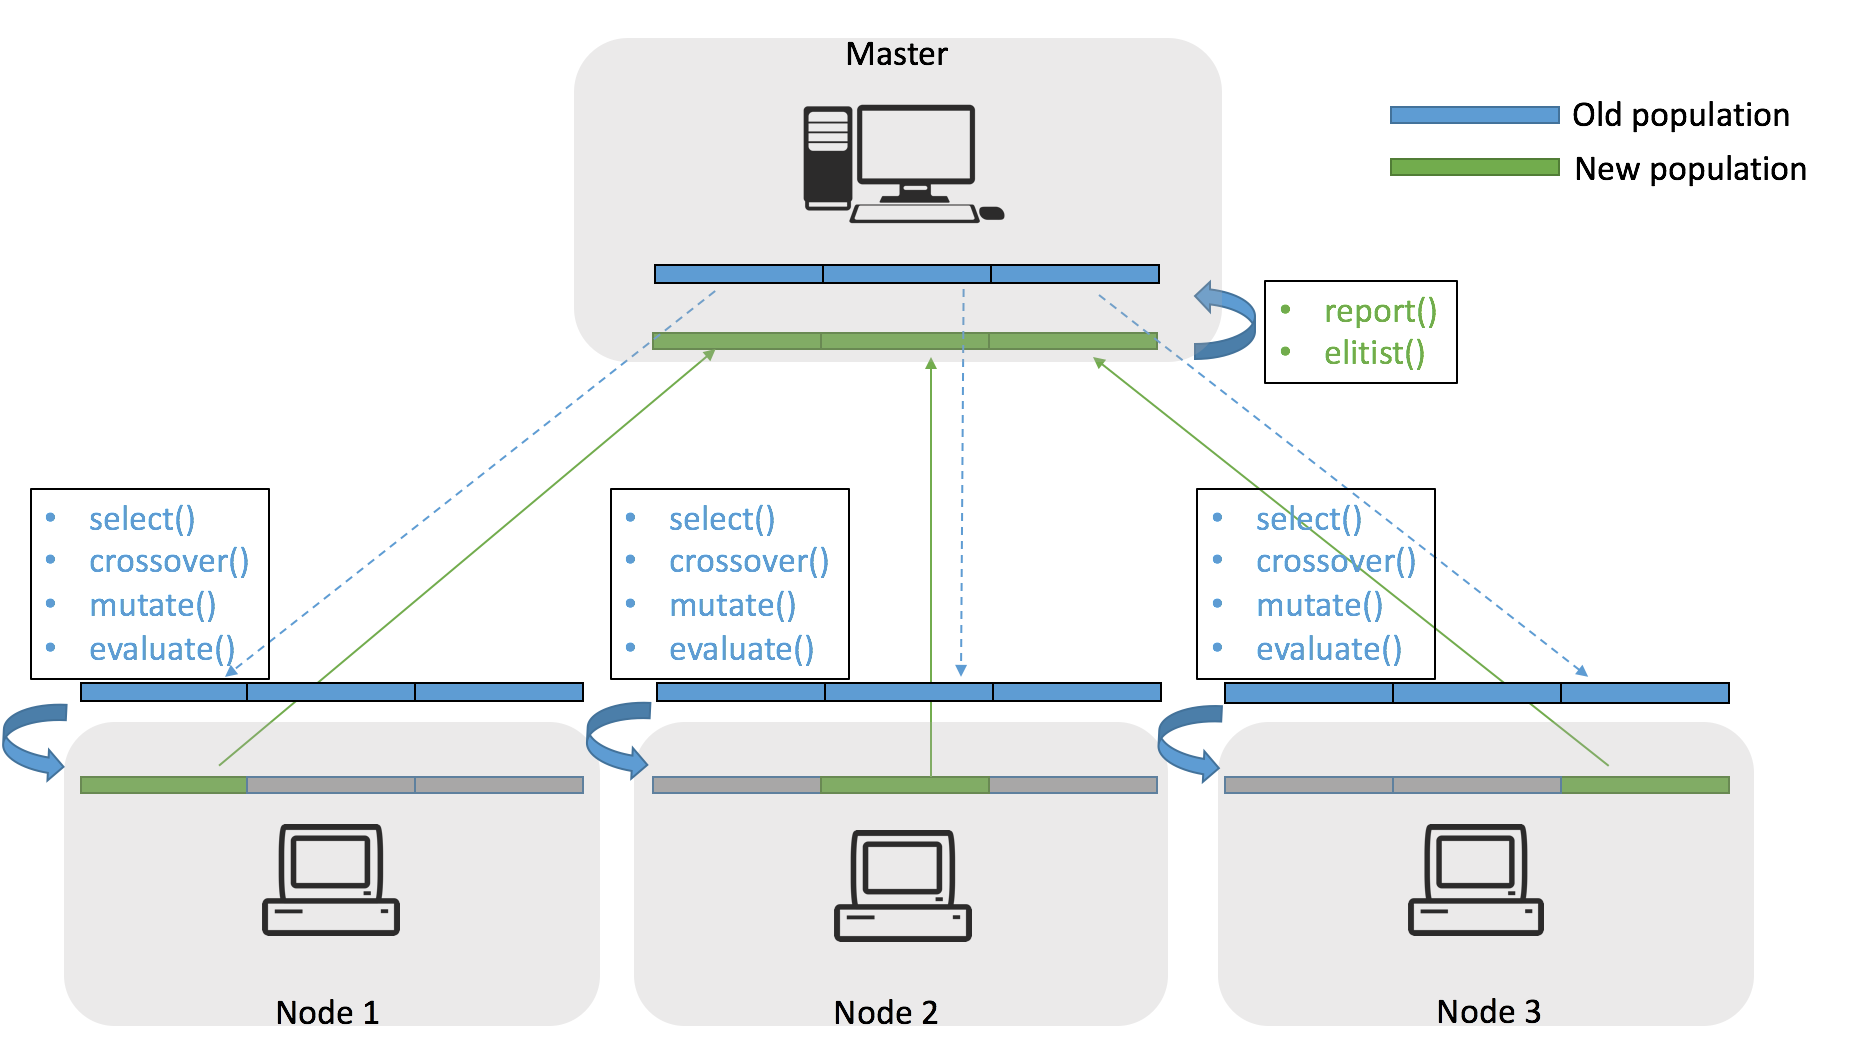
\includegraphics[width= \linewidth]{figs/pga_model_v2.png}
    \caption{PGA v2 model}
     \label{fig:pga_model_v2}
\end{figure}

\subsubsection{Using MPI Broadcast instead of explicit MPI Send/Recv}
To reduce communication overhead MPI collective routine \textbf{MPI\_Bcast()} is used by replacing  explicit \textbf{MPI\_Send() and MPI\_Recv()}. To ensure proper synchronisation among all nodes in the cluster the \textbf{MPI\_Barrier()} is called. When a process calls MPI\_Barrier(), it waits until all of the nodes also call this procedure.

Some part of this implementation is shown in Listing \ref{lst:pga_procedures}. On lines 5-9 master node initialises initial population and perform first elitist operation(keep\_the\_best( )). Slave nodes wait for these operation to complete because of MPI\_Barrier() call on line 12. On line 15 entire population is broadcasted with MPI\_Broadcast() call followed by another call to MPI\_Barrier().  On lines 20-21 all nodes determine their own data partition information. Then all nodes perform GA operations and evaluate the fitness values for the subpopulation(lines 22-27). On lines 32-36 each node then broadcasts its part of the population data. This followed by another synchronisation on line 38 before master node call the elitist() operation on entire population on line 43.

\begin{lstlisting}[language=C, caption={PGA v2 main() procedures.}, label={lst:pga_procedures}]
ierr = MPI_Comm_size(MPI_COMM_WORLD, &numNodes); // How many nodes
ierr = MPI_Comm_rank(MPI_COMM_WORLD, &myId); // My Rank ID
    
/* Initialise first gen population in master process */   
if(myId == MASTER_ID) // Master Process
{        
      initialize ( filename, seed );
      evaluate (0, POPSIZE );
      keep_the_best ( );
}

MPI_Barrier(MPI_COMM_WORLD);
   
/* Broadcast entire first generation from master process */
MPI_Bcast(population, POPSIZE + 1, mpi_genotype, MASTER_ID, MPI_COMM_WORLD);
   
MPI_Barrier(MPI_COMM_WORLD);
 
/* Each process does GA ops here on individual data parts */ 
int my_start = nodes_data[myId][0];
int row_count = nodes_data[myId][1];
for ( generation = 0; generation < MAXGENS; generation++ )
{      
     node_selector (my_start, row_count, seed );
     crossover ( seed );
     node_mutate ( my_start, row_count,seed );   
     evaluate (my_start, row_count);
         
       /* Sync message - 3 */
      MPI_Barrier(MPI_COMM_WORLD);
        
      for(int i = 0; i < numNodes; i++)
      {
          MPI_Bcast(&population[nodes_data[i][0]], nodes_data[i][1], mpi_genotype, i, MPI_COMM_WORLD);
          MPI_Barrier(MPI_COMM_WORLD);
      }
        
      MPI_Barrier(MPI_COMM_WORLD);
        
      if(myId == MASTER_ID) // Master Process
      {
          report(generation);
          elitist ( );
      }
        
      MPI_Barrier(MPI_COMM_WORLD);
}
\end{lstlisting}

\subsection{PGA v3}

\subsubsection{Running Time Analysis of node\_selector() Procedure}
\label{pga_runtime_analysis}
During empirical study of program running time, with PGA v2 we noticed some performance gain when number of processors are increased for smaller population size(5000). We also noticed there is a drop of speedup when population size is increased.

After a some investigation into this problem it was identified that the running time of \textbf{selector()} procedure is contributing for this unexpected result. The Listing \ref{lst:pga_select} parts of this procedure where we can see there is a nested for loop. The outer loop(line 2) on line has a range of \textit{$(0, n/p)$} and the inner loop(line 11) has a range of  \textit{$(0, p)$} where  \textit{n} is the population size and \textit{p} is number of processors. Thus this function has a running time complexity of $\mathcal{O}(n/p * n)$ which is essentially $\mathcal{O}(n^2)$.

Since, all nodes are executing this node\_selector() procedure using entire global population, the total running time is directly dependent upon the slowest node/processor in the cluster plus communication overheard for each generation cycles.


\begin{lstlisting}[language=C, caption={node\_select() procedure.}, label={lst:pga_select}]
/* Select survivors using cumulative fitness. */ 
for ( i = my_start; i < ends; i++ )
{ 
    p = r8_uniform_ab ( a, b, seed );
    if ( p < population[0].cfitness )
    {
        newpopulation[i] = population[0];   
    }
    else
    {
        for ( j = 0; j < POPSIZE; j++ )
        {
            if ( population[j].cfitness <= p && p < population[j+1].cfitness )
            {
                newpopulation[i] = population[j+1];
            }
        }
    }
}
\end{lstlisting}


\subsubsection{Limiting Selection to Partial Population}
Based on the analysis discussed above, in this implementation the \textbf{selector()} procedure is modified so that the selection is done using nodes local subpopulation. Thus this would result in running time complexity of $\mathcal{O}((n/p) * (n/p))$ i.e . $\mathcal{O}((n/p)^2)$ Theoretically, if we could add more nodes i.e. processors we could reduce the affect of population size increases for this procedure proportionally. We know that number of processor cannot always be matched with population size increases but for a reasonably large population size (not infinite), adding in extra nodes can reduce the running time complexity of this function significantly. Figure \ref{fig:pga_model_v3} shows the data partition and GA operation for master and slave nodes. All GA operation including selection is done on subpopulation.

\begin{figure}[!htb]
        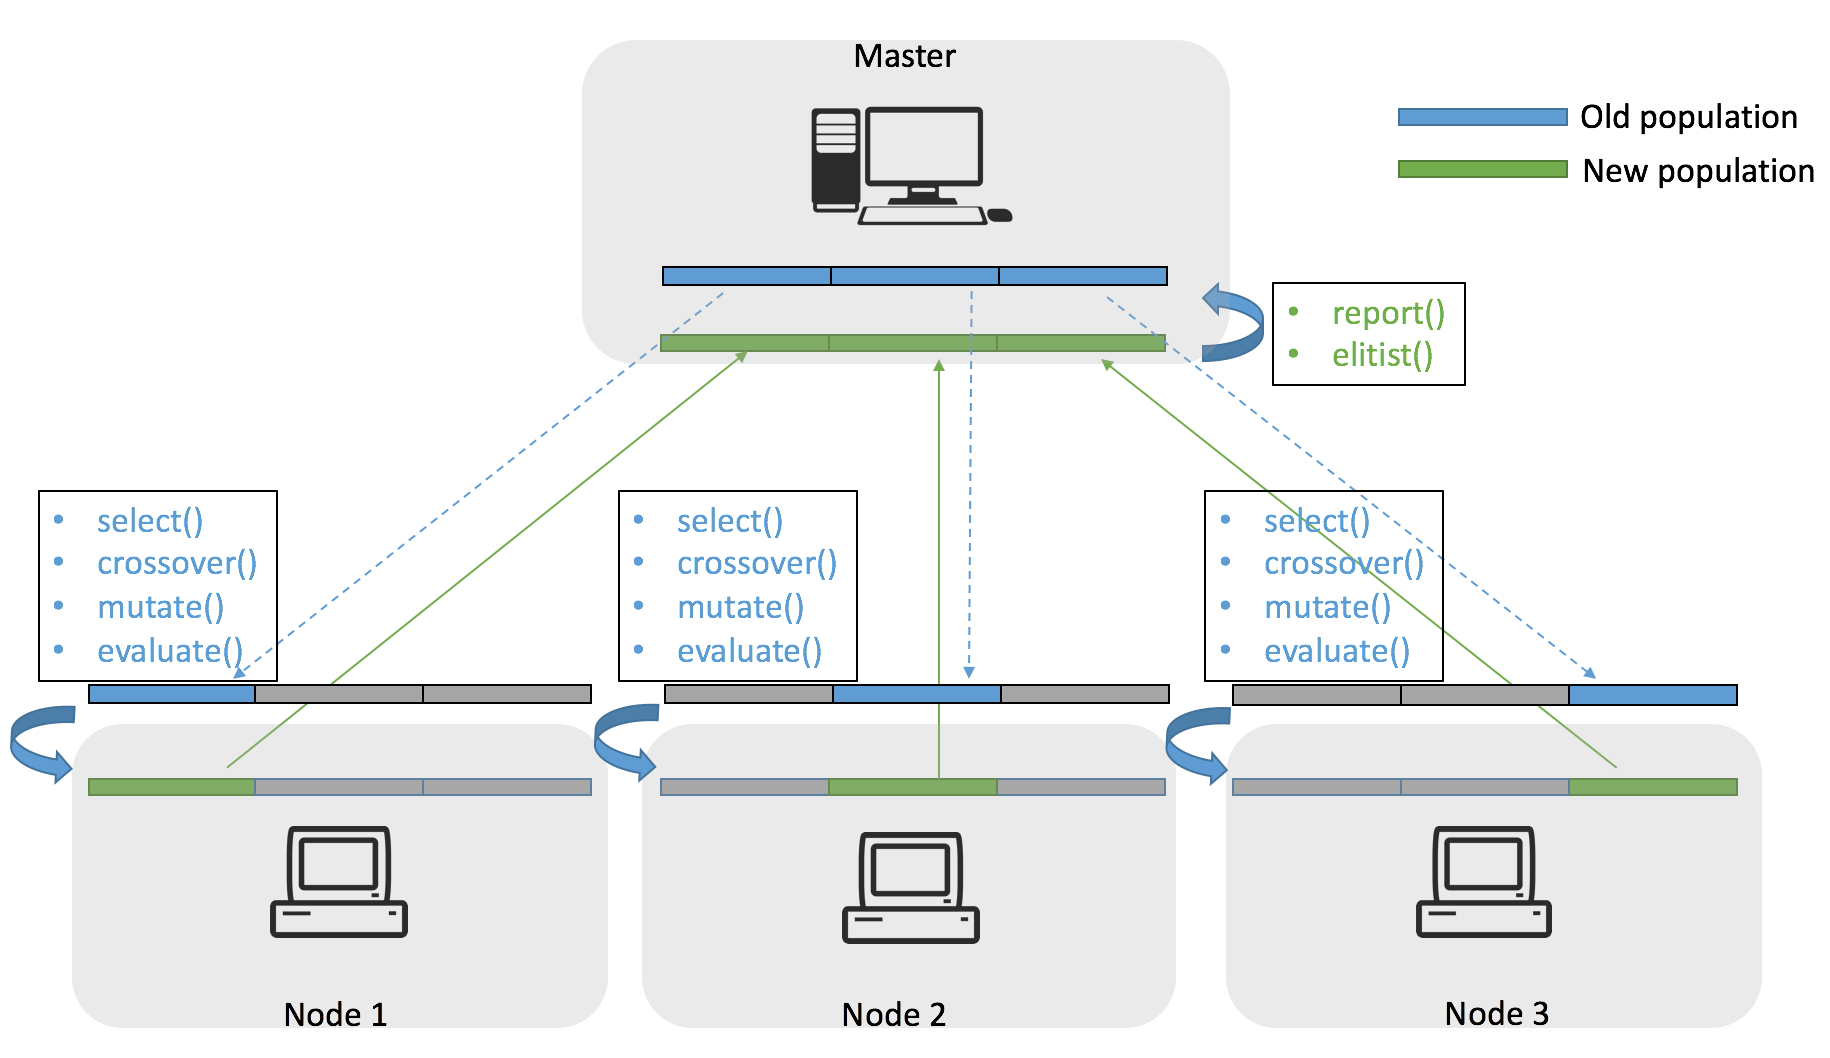
\includegraphics[width= \linewidth]{figs/pga_model_v3.png}
    \caption{PGA v3 model}
     \label{fig:pga_model_v3}
\end{figure}

Changes to the selector functions are shown in Listing \ref{lst:pga_select_changes} where the range inner for loop at line 10 is limited for the local subpopulation only which gives a range of \textit{$(0, n/p)$}.

\begin{lstlisting}[language=C, caption={Changes made in node\_select() procedures.}, label={lst:pga_select_changes}]
for ( i = my_start; i < ends; i++ )
{ 
    p = r8_uniform_ab ( a, b, seed );
    if ( p < population[my_start].cfitness )
    {
        newpopulation[i] = population[my_start];      
    }
    else
    {
        for ( j = my_start; j < ends; j++ )
        { 
            if ( population[j].cfitness <= p && p < population[j+1].cfitness )
            {
                newpopulation[i] = population[j+1];
            }
        }
    }
}
\end{lstlisting}

\subsection{Issues with Serialising Dynamic Data}
The SGA implementation allows population size, number of variables in a chromosome and number of generation can only be modified at compile time. To carry out the experiments we needed the PGA accept these parameters at runtime. So, an attempt was made to change these parameters at runtime with command line arguments. After a week of trials, this attempt was unsuccessful because of a number of reasons which are discussed here. Part of the problem was due to the data structure chosen to represent the chromosome which contains three static array members. The length of these arrays are defined at compile time. Population are initialised inside initialize\(\) procedure (Listing \ref{lst:initialize_proc}). Each individual is initialised with random permissible value. In this trial changes were made to the genotype data structure so that it could be initialised with dynamic arrays using malloc(). Program was compiled normally without any error. But during testing the PGA failed to produce acceptable outcome.

To find the underlying issue GDB was used to debug the problem. During this debugging program was run with a population size of 5. So the best member of a generation is kept  at index 5.
 
It was noticed(GDB output - Listing \ref{lst:gdb_output}) that some values of population members were changing unexpectedly. As we can see from the source code given in Appendix \ref{src:sga_proc.cpp} the initialize() procedure only assign initial value for \textbf{lbound}, \textbf{ubound} and \textbf{gene}. In this debugging session, the values of i, j and the best individual(population[5]) was monitored to catch unexpected any change. On line 42 we see that the value of  population[5].gene is 0x626330. But on next step on line 54 this value has changed to 0x3fe197d48c1f329c. We know that the initialize() procedure only assign values for the population member from 0 to (POPSIZE - 1) which is 4 in this run. So, the changes in population[5] is unexpected. It appeared that even though no value was assigned for best individual (which is population[5]), its member's values were changing. After looking more closely, it was noticed that the value that was being assigned to a data member for one individual was appearing inside some other individual's data member. Which means values were being assigned into wrong memory location. This indicated that malloc() for initialising the population array was not correct.


\begin{lstlisting}[style=BashInputStyle, label={lst:gdb_output}]
847 population[j].gene[i] = r8_uniform_ab ( lbound, ubound, seed );
1: population[5] = {fitness = 0, rfitness = 1.6304166312761136e-322, 
_ cfitness = 0, gene = 0x626330}
2: i = 0
3: j = 2
(gdb) 
840 for ( j = 0; j < POPSIZE; j++ )
1: population[5] = {fitness = 0, rfitness = 1.6304166312761136e-322, 
_ cfitness = 4.147546169663503, gene = 0x626330}
2: i = 0
3: j = 2
(gdb) 

.....

840 for ( j = 0; j < POPSIZE; j++ )
1: population[5] = {fitness = 0, rfitness = 1.6304166312761136e-322, 
_ cfitness = 4.147546169663503, gene = 0x626330}
2: i = 1
3: j = 1
(gdb) 
842 population[j].fitness = 0;
1: population[5] = {fitness = 0, rfitness = 1.6304166312761136e-322, 
_ cfitness = 4.147546169663503, gene = 0x626330}
2: i = 1
3: j = 2
(gdb) 
843 population[j].rfitness = 0;
1: population[5] = {fitness = 0, rfitness = 1.6304166312761136e-322, 
_ cfitness = 4.147546169663503, gene = 0x626330}
2: i = 1
3: j = 2
(gdb) 
844 population[j].cfitness = 0;
1: population[5] = {fitness = 0, rfitness = 1.6304166312761136e-322, 
_ cfitness = 4.147546169663503, gene = 0x626330}
2: i = 1
3: j = 2
(gdb) 
847 population[j].gene[i] = r8_uniform_ab ( lbound, ubound, seed );
1: population[5] = {fitness = 0, rfitness = 1.6304166312761136e-322, 
_ cfitness = 4.147546169663503, gene = 0x626330}
2: i = 1
3: j = 2
(gdb) 
840 for ( j = 0; j < POPSIZE; j++ )
1: population[5] = {fitness = 0, rfitness = 1.6304166312761136e-322, 
_ cfitness = 4.147546169663503, gene = 0x3fe197d48c1f329c}
2: i = 1
3: j = 2
(gdb) 
842 population[j].fitness = 0;
1: population[5] = {fitness = 0, rfitness = 1.6304166312761136e-322, 
_ cfitness = 4.147546169663503, gene = 0x3fe197d48c1f329c}
2: i = 1
3: j = 3
\end{lstlisting}

After this discovery, one and half week time was spent on how to allocate memory correctly for the \textbf{genotype} struct. But it seemed quite complicated to do so with three variable length array members in a struct. By researching on Internet about this, it was found that this issue is known as Variable Length Array In Struct(VLAIS). And with further research, some discussions related to this topic was found in Stackoverflow. The suggestions there were indicating that VLAIS is permissible on specific compiler i.e GCC C99 compatible only.  In one discussion posted on Stackoverflow \footnote{http://stackoverflow.com/questions/21804994/using-a-struct-member-as-array-size-in-the-same-struct} related to this topic further suggested that that variable-length arrays in structs is permissible in gcc (and the newest C-standards), but the variable array must always be the last member of the struct (so the compiler knows where all members are). In particular this means:

\begin{enumerate}
	\item There can be only one variable-length array
	\item If the struct is a member of another struct, it has to be the last member of that struct.
\end{enumerate}

Another post \footnote{http://stackoverflow.com/questions/17552312/multiple-flexible-array-in-a-struct-in-c} also suggested that it is not possible to have more than one flexible-array member in a struct.

There is no clear information whether mpic++ compiler has support for this feature of gcc too or not. The alternative solution to this problem would be to replace struct data structure with combination of C++ objects and vectors. Since this would have involved making a considerable changes to actual SGA implementation and possibilities of going back to the earlier problem with Object-oriented GA, a decision was made to leave these parameters to be defined at compile time.

\chapter{Design and Implementation}

\section{Introduction}
In this chapter all aspects of design and implementation that were done for this project are discussed. A parallel infrastructure was essential for this project for implementing the PGA using Message Passing Interface. A considerable time and effort were made to implement and configure the Beowulf cluster to facilitate the parallel infrastructure for the project. Our original idea was to use an existing Beowulf system in University's laboratory. Later it was discovered that, the most of the hardware of that Beowulf system were dismounted and no longer suitable for this project. So, the the most obvious alternative was to build a Beowulf cluster for this project. At first, a virtual Beowulf system was simulated on a dual core MacBook. Then an actual hardware based Beowulf system was implemented using multiple old PC's. After all, this is the noble idea of a Beowulf system to have it built using hardware laying around  that have very little or no use at all.

Another important part of implementing a PGA, we needed to identify a suitable existing SGA implementation. Even though the Genetic Algorithm was not the centre theme of this project, it was very important to do a considerable background studies in GA to understand the underlying concepts well. It was also important to understand and identify different techniques of parallelising GAs. Much efforts and time were put into understanding two different implementation of SGA and their suitability on parallelising using MPI in details for this project which are discussed in this chapter.

With PGA implementation, we were faced with many issues and challenges. Some of these issues were identified during PGA implementation and some were identified during empirical studies. Which resulted in implementing 3 versions of PGA. 

A lot efforts were made to create prototypes using python scripts to gather experiments data and use gnuplot to visualise the results to compare and contrast to validate the hypotheses relating to PGA performance.

\section{Setting up the Beowulf Cluster}
\label{beowulf_setup}
\subsection{Cluster components}
Computer cluster is made up of various hardware and software components with complex interactions between different components. Figure \ref{fig:cluster-layers} depicts the various components that form a cluster.

\begin{figure}[!htb]
 \center
  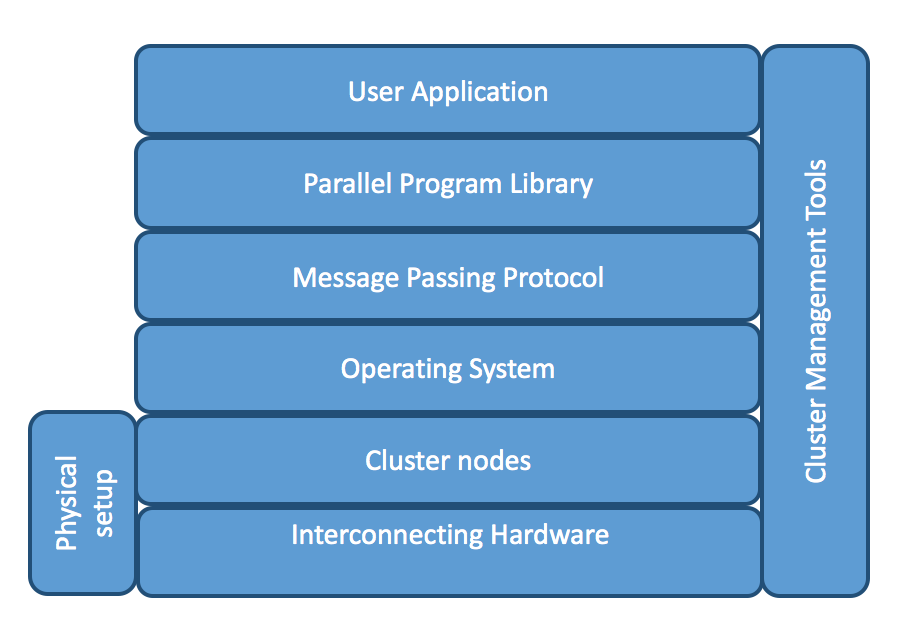
\includegraphics[width= .75 \linewidth]{figs/cluster/cluster_layers.png}
  \caption{Layers in a Cluster}
  \label{fig:cluster-layers}
   \center
\end{figure}

A Beowulf cluster contains a set of cluster nodes. A node can be a server with a specific role within the cluster or it can be a compute node. All of the nodes are connected using a dedicated Local Area Network(LAN) or System Area Network(SAN). The complexity of networking topology is depends on directly to number of nodes in the cluster.

As shown in Figure \ref{fig:cluster-layers} to setup a cluster we need following hardware and software components:

\paragraph{Cluster Nodes}
Cluster nodes are stand-alone computers with one or more CPUs, own Memory unit, and Network Interface Card(NIC). A node may contain it's own local secondary storage or could be configured as disk-less workstation. For this implementation nodes were configured with their own local storage to reduce network overhead for accessing boot-image and runtime libraries during boot up and program execution. However, Network File Sharing(NFS) was implemented to streamline program execution environments across the Cluster. The details of nodes configurations are discussed later in this chapter for both virtual and physical implementation.

\paragraph{Interconnecting Hardware}
This is networking components of the cluster that facilitates nodes communicating with one another. Since communication is the key part of cluster computing this is very important component that can define the overall performance. For this project a simple ethernet network was configured for both virtual and physical implementation. For the physical setup, Thompson Broadband Router (Model: TWG870) was used. This router has 4 Gigabit ports that facilitated to setup a Gigabit LAN for the cluster-only network.

\paragraph{Operating System}
Linux is widely used on Beowulf cluster because of its hardware support, performance, its free and open source kernel. For this project Ubuntu Server 16.04 was chosen.

\paragraph {Message Passing Protocol}
There are two typical approaches to communication between cluster nodes, one is  Parallel Virtual Machine(PVM) and the other is Message Passing Interface (MPI). However, MPI has now emerged as the de facto standard for message passing on computer clusters. The objective of this project is parallelising SGA using MPI libraries therefore, MPI was chosen message passing protocol for obvious reason.

\paragraph {Parallel Program Library}
MPI has many implementation. There are two free and popular MPI libraries available, one is OpenMPI and another is MPICH. For this project MPICH 3.2 is installed on each nodes. 

\paragraph {Cluster management tools}

\subsection{Topological design}
Figure \ref{fig:beowulf-cluster} shows a simple Beowulf cluster setup that was adopted for this project implementation. For simplicity the implemented Beowulf contains a Master node and 3 to 4 compute nodes which is extendable.

\begin{figure}[!htb]
  \includegraphics[width=\linewidth]{figs/cluster/beowulf_cluster.png}
  \caption{A typical Beowulf setup}
  \label{fig:beowulf-cluster}
\end{figure}

Beowulf cluster was simulated in virtual environment using Oracle VirtualBox and then actual hardware implementation was done using commodity physical hardware. In both cases the software suits and configuration was identical with minor changes.

\subsection{Virtual nodes}
Table \ref{tab:virt_node_conf} shows the node configuration when using simulated hardware using VirtualBox on Macbook Pro(2.6GHz Intel core i5, 16 GB RAM, 256GB SSD) host computer.

%% Node description table 
\begin{table}[!htb]
\centering
\caption{Virtual nodes configuration}
\begin{tabular}{|l|l|l|l|}
\hline
Hostname & Role & IPv4 address & Hardware Config \\ \hline
master & Master & 192.168.56.10/24 & Single core, 2GB RAM, 10 GB HDD \\ \hline
node1 & Slave & 192.168.56.11/24 & Single core, 2GB RAM, 10 GB HDD \\ \hline
\end{tabular}
\label{tab:virt_node_conf}
\end{table}

\subsection{Physical nodes}
Table \ref{tab:phy_node_conf} shows the node configuration of using physical components. 
%% Physicle node description table 
\begin{table}[!htb]
\centering
\caption{Physical nodes configuration}
\begin{tabular}{|l|l|l|l|}
\hline
Hostname & Role & IPv4 address & Hardware Config \\ \hline
padma & Master & 172.16.0.1/24 & Dell Dual-core, 6GB RAM, 160 GB HDD \\ \hline
meghna & Slave & 172.16.0.15/24 & HP Dual-core, 2GB RAM, 160 GB HDD \\ \hline
jamuna & Slave node & 172.16.0.17/24 & HP Dual-core, 2GB RAM, 160 GB HDD \\ \hline
\end{tabular}
\label{tab:phy_node_conf}
\end{table}

\afterpage{\clearpage}

\subsection{Setup \& Configuration}
\subsubsection{Setup steps}
\begin{itemize}
	\item Install Operating Systems(OS) for each nodes
	\item Configure network settings
	\item Create MPI user
	\item Configure Network File Share
	\item Configure SSH password-less login
	\item Install MPI libraries, compiler and build tools
	\item Administrative tasks
\end{itemize}

\subsubsection{Installing Operating System} 
Popular Linux distribution Ubuntu Server 16.04 was chosen as OS for all cluster nodes. It was installed with default settings and without any GUI or window manager. A desktop environment was not needed as it would have reduced the performance of our Beowulf system. Therefore our installation of Ubuntu Linux was a minimal system and OpenSSH server.

After a successful installation of the operating system, we needed to set up the network and, of course, the shared file system for the compute nodes. For the shared file system, we installed the NFS server on the first node, which operates as the head node. Then, we exported the locations for the shared file system from there.

\subsubsection{Network configuration - Master node}

Identify network interface card and its name
\begin{lstlisting}[style=BashInputStyle]
$ip link show
\end{lstlisting}

And from the output shown as below we identify the NIC names that we want to configure in following steps

%\begin{lstlisting}[style=BashInputStyle, caption={Network device configuration file}, label={lst:config_net_dev}]
\begin{lstlisting}[style=BashInputStyle]
1: lo: <LOOPBACK,UP,LOWER_UP> mtu 65536 qdisc noqueue state UNKNOWN mode DEFAULT group default qlen 1
    link/loopback 00:00:00:00:00:00 brd 00:00:00:00:00:00
2: enp2s0: <BROADCAST,MULTICAST,UP,LOWER_UP> mtu 1500 qdisc pfifo_fast state UP mode DEFAULT group default qlen 1000
    link/ether ec:08:6b:04:62:df brd ff:ff:ff:ff:ff:ff
3: enp0s25: <BROADCAST,MULTICAST,UP,LOWER_UP> mtu 1500 qdisc pfifo_fast state UP mode DEFAULT group default qlen 1000
    link/ether 00:19:d1:73:38:60 brd ff:ff:ff:ff:ff:ff
\end{lstlisting}

To configure the network configuration file /etc/network/interfaces need to be edited as follows:
\begin{lstlisting}[style=BashInputStyle]
auto lo
iface lo intet loopback

# The primary network interface(connected to public network)
auto enp0s25
iface enp0s25 intet static
	address 192.168.0.14
	netmask 255.255.255.0
	gateway 192.168.0.1
	dns-nameserver 89.101.160.5  8.8.8.8

# The cluster network interface
auto enp2s0
iface enp2s0 intet static
	address 172.16.0.1
	netmask 255.255.255.0
\end{lstlisting}

System's host file( /etc/hosts ) needs to be edited for each node for easier host look up.

\begin{lstlisting}[style=BashInputStyle]	
127.0.0.1	localhost
172.16.0.1	padma
172.16.0.2	meghna
172.16.0.3	jamuna
\end{lstlisting}

Then scp this file to other nodes and copy it with privileged user into /etc directory.

\begin{lstlisting}[style=BashInputStyle]
	$scp /etc/hosts meghna:~/
	$ssh meghna
	$sudo cp hosts /etc/hosts
	$scp /etc/hosts jamuna:~/
	$ssh jamuna
	$sudo cp hosts /etc/hosts
\end{lstlisting}

\subsubsection{Create MPI user}
Create a user for running MPI jobs. This user needs to created with same user ID and group ID on each node.

\begin{lstlisting}[style=BashInputStyle]
	$sudo adduser mpiuser --uid 999
\end{lstlisting}

\subsubsection{Network File System configuration}

Install and setup the Network File System
\begin{lstlisting}[style=BashInputStyle]
# Master node
padma$ sudo apt-get install nfs-kernel-server
padma$ sudo apt-get install nfs-common
# And compute nodes
meghna$ sudo apt-get install nfs-common
jamuna$ sudo apt-get install nfs-common
\end{lstlisting}

Next we need to share mpiuser home directory with all other nodes. To do this the file /etc/exports on the master node needs to be edited to add the share directory.

\begin{lstlisting}[style=BashInputStyle]
	/home/mpiuser 172.16.0.0/24(rw,sync,no_subtree_check)
\end{lstlisting}


At this point NFS server needs to be restarted to make share directory available across the network.

\begin{lstlisting}[style=BashInputStyle]
master:~\$ sudo service nfs-kernel-server restart
sudo exportfs -a
\end{lstlisting}

Now we can check and confirm from compute node if the NFS shared directory can be mount.

\begin{lstlisting}[style=BashInputStyle]
	showmount -e padma
\end{lstlisting}

This should show the export list from master node as below:
\begin{lstlisting}[style=BashInputStyle]
Export list for padma:
/home/mpiuser 172.16.0.0/24
\end{lstlisting}

To mount this shared directory from other nodes we can execute the command below from the shell.

\begin{lstlisting}[style=BashInputStyle]
meghna:~\$ sudo mount master:/home/mpiuser /home/mpiuser
jamuna:~\$ sudo mount master:/home/mpiuser /home/mpiuser
\end{lstlisting}

And to mount the share directory at system boot up without having to enter the command manually, the following entry is added to all compute nodes in the file /etc/fstab.

\begin{lstlisting}[style=BashInputStyle]
	padma:/home/mpiuser /home/mpiuser nfs
\end{lstlisting}

\subsubsection{Configure password less communication}
All MPI nodes should be able to communicate with other nodes without having to provide any password. This is achieved by configuring password-less SSH between nodes.

If ssh is not installed with during the OS installation steps we could install it by running the following command on each nodes:
\begin{lstlisting}[style=BashInputStyle]
	$sudo apt-get install ssh
\end{lstlisting}

Next step is to generate a SSH key for  'mpiuser' on all nodes. The SSH key is by default created in the user's home directory. In our case the 'mpiuser' home directory  which is located at /home/mpiuser. This is actually the same directory for all nodes i.e  /home/mpiuser on the master node since the home directory is a NFS mount. So, the SSH key for the 'mpiuser' was generated on master node, and all other nodes will automatically have an SSH key in 'mpiuser' home directory. 

To generate an SSH key for the MPI user on the master node (but any node should be fine).
\begin{lstlisting}[style=BashInputStyle]
	\$ su mpiuser
	\$ ssh-keygen
\end{lstlisting}

When asked for a passphrase, this needs to be left empty (hence password-less SSH).

When done, the 'mpiuser' should have same ssh-key on its home directory which is accessible from all nodes in the cluster. Now, the master node needs to be able to automatically login to the compute nodes. To enable this, the public SSH key of the master node needs to be added to the list of known hosts (this is usually a file \~/.ssh/authorized\_keys) of all compute nodes. All SSH key data is stored in one location: /home/mpiuser/.ssh/ on the master node. So instead of having to copy master node's public SSH key to all compute nodes separately, we just have to copy it to master's own authorized\_keys file. There is a command to push the public SSH key of the currently logged in user to another computer. To do that we run the following commands on the master node as user "mpiuser",
\begin{lstlisting}[style=BashInputStyle]
	mpiuser@master:~\$ ssh-copy-id localhost
\end{lstlisting}

Master node's own public SSH key should now be copied to /home/mpiuser/.ssh/authorized\_keys. But since /home/mpiuser/ (and everything under it) is shared with all nodes via NFS, all nodes should now have master's public SSH key in the list of known hosts. This means that we should now be able to login on the compute nodes from the master node securely without having to enter a password,

\begin{lstlisting}[style=BashInputStyle]
	mpiuser@master:~$ ssh meghna
	mpiuser@meghna:~$ echo $HOSTNAME
	meghna
\end{lstlisting}

The user 'mpiuser' should be now be able to login on node1 via SSH. At this stage login to other nodes also be checked.

\subsubsection{Install MPI libraries, compiler and build tools}
On each node we needed to install C/C++ libraries and headers files along with required build tools. After that we installed MPICH 3.2 version of MPI library using Ubuntu's default source repository.

\begin{lstlisting}[style=BashInputStyle]
	$sudo apt-get install build-essential
	$sudo apt-get install mpich
	$mpicc -v  \# To check MPICH version OR
	$mpiexec --version
\end{lstlisting}

\subsubsection{Configuring MPI Process Manager}
\label{beowulf:process_manager}
A process manager is needed for MPI programs are to spawn and manage parallel cluster. This process manager is an external entity. In MPICH implementation of MPI library these process managers communicate with MPI processes using a predefined interface called as PMI (Process Management Interface). The process manager included with MPICH 3.2 installation is called Hydra.
In order to setup Hydra, we need to create one file on the master node. This file contains all the host names of the compute nodes. This file can be put in anywhere, but for simplicity it is created in the the MPI user?s home directory. This file only needs to be present on the node that will be used to start jobs on the cluster, usually the master node. Hydra uses this file to spawn process in the cluster in round robin manner. Since the MPI home directory is shared among all nodes, all nodes will have the hosts file. This file is created using following command where the file is named \textit{hosts}:

\begin{lstlisting}[style=BashInputStyle]
	$cd ~
	$touch hosts
\end{lstlisting}

For this Beowulf setup the following entries are added to this \textit{hosts} file: 
\begin{lstlisting}[style=BashInputStyle]
padma:2
meghna:2
jamuna:2
\end{lstlisting}



\section{Object-Oriented GA}
There are many different implementation of Simple Genetic Algorithms(SGA) available. Initially the SGA implementation selected for this project for parallelising was an implementation that closely followed the suggestions of David E. Goldberg's book \textit{"Genetic Algorithms in Search, Optimization, \& Machine learning"} \citep{Goldberg:89}. It was implemented using C++ and took an Object Oriented approach as an abstraction mechanism. There are 37 user modifiable parameters defined to fine tune the behaviour the SGA. It was designed to allow users to change the chromosome structure(haploid or diploid), fixed or variable length chromosome, 3 different mechanism of diploid crossovers, 7 different types of encoding schemes. User could also select fitness function from 15 different implementation(even though only a few of them are actually implemented). It also allows user to select from two different models of elitism, 6 different mechanism of selections. Furthermore, it contains an implementation of Linear Congruential method for generating pseudo random numbers which is used to randomly generate probabilities for mutation and crossover.

This codebase contains over 4,500 lines of code. About 2 weeks time was spent on compiling and running this SGA to understand different parameters and process flow of the algorithm it had implemented. Which was well beyond the planned schedule for this project that is shown in Project plans in Appendix \ref{appendix:project_plans}.

After 2 weeks of studying and experimenting with this SGA implementation, I managed to summarise an analysis of this implementation. this code exhibit many OOD(Object Oriented Development) pitfalls that was common in early Object Oriented Development days. Inheritance was used as a means of implementation reuse without any semantic coherence. Classes are too big and contains too many responsibilities which is against "Single Responsibility principle" of OOD. In many cases, classes violates Liskov's Substitute Principle as well where a derived classes cannot be replaced for the base classes.
Figure \ref{fig:sga_classdiagram} shows the class diagram of this implementation of SGA code using C++.
 

\begin{figure}[!hp]
    \vspace*{-1.5cm}
    \makebox[\linewidth]{
        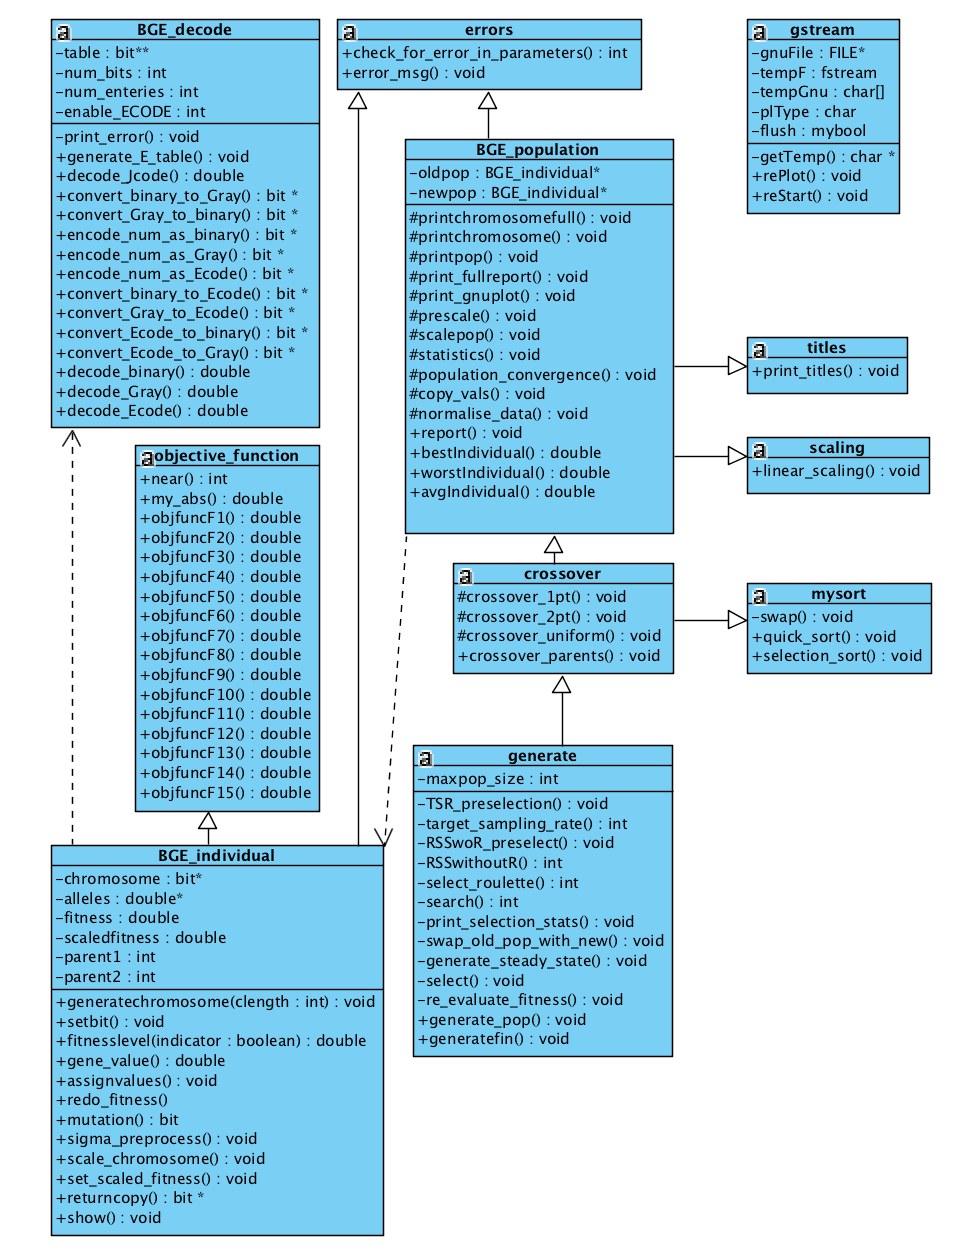
\includegraphics[width=1.3\linewidth]{figs/sga_class_diagram.png}
    }
    \caption{Class diagram of Object-oriented SGA}
     \label{fig:sga_classdiagram}
\end{figure}

\section{Issues with MPI support for Object-oriented paradigm}
The major drawback discovered with object-oriented implementation of GAs was the MPI's lack of support for object-oriented languages. The MPICH 3.2 version of MPI implementation were used this project. With further research on this topic it was discovered none of the major MPI implementation(OpenMPI, ) truly supported the object-oriented C++ other than just the compiler support.

In a conference article titled \textit{"Object Oriented MPI (OOMPI): a class library for the Message Passing Interface"} Squyres et al discussed MPI's lack of support of C++ class libraries and binding. In that paper they suggested an Object Oriented MPI specification \citep{squyresoompi}. However, this effort have been abandoned due to the lack of support from MPI community. After doing further research on this topic in Internet discussion forums and blog posts, it is found that there are ways of doing OO MPI using C++ by using third-party libraries Boost::mpi and Boost::serialization. Boost itself is a set of libraries for the C++ programming language that provide support for tasks and structures such as linear algebra, pseudorandom number generation, multithreading, image processing, regular expressions, and unit testing. Boost is a free to use library licensed under its own free, open-source license, known as the Boost Software License. An MPI program using the Boost::mpi library must initialise an mpi::environment object. This object initialises the MPI environment and enables communication among the processes. This object is initialised with the program arguments in the main program. The creation of this object initialises the MPI environment, and its destruction terminates it. The Boost::mpi requires objects to be serialised so that they are transmissible across processes. The Boost::serialization is a library for serialising C++ objects for sending/receiving data across network. To serialise a class one needs to define a template function serialize() in the class.

There is a little draw back with using Boost::mpi library. The Boost:mpi only implemented MPI1.1 which does not support many useful routines of MPI standards. Some people suggested to use that for regular programs. And for advanced programs to use mainstream MPI-3 libraries with Boost::Serialization for serialising C++ objects. Considering the scope of this project this options is not taken.
\section{Open Source Procedural GA}
A procedural implementation of GA based on Zbigniew Michalewicz's book \textit{"Genetic Algorithms + Data Structures = Evolution Programs"}\citep{michalewicz:96} available under GNU public license. The original version of this implementation was done by Dennis Cormier and Sita Raghavan. From Department of Scientific Computing at Florida State University John Burkardt made a C++ version of source code available on their department's website \citep{Burkardt:17}. The slightly refactored version of this source code without changing the actual algorithms is included in Appendix \ref{sourcecodes}. Where the original code is put into 4 separate source files shown in \ref{src:params.hpp}, \ref{src:sga_proc.hpp}, \ref{src:sga.cpp} \& \ref{src:sga_proc.cpp}.


This is a simple genetic algorithm implementation where the evaluation function takes positive values only and the fitness of an individual is the same as the value of the objective function.

Each generation involves selecting the best members, performing crossover and mutation and then evaluating the resulting population, until the terminating condition is satisfied.

Behaviour of this program is modified by defining parameters listed in Listing \ref{lst:procedural_ga_params} where POPSIZE is population size, MAXGEN is the number of generation to run, NVARS is the number of variables or genome in a chromosome, PXOVER and PMUTATION are the probabilities of crossover and  mutation respectively. However this program expects the permissible value ranges for each variable to be read from a text file.

\begin{lstlisting}[language=C, caption={Parameter definitions.}, label={lst:procedural_ga_params}]
# define POPSIZE 50
# define MAXGENS 1000
# define NVARS 3
# define PXOVER 0.8
# define PMUTATION 0.15
\end{lstlisting}

Listing \ref{lst:procedural_ga_struct} shows the data structure used for defining GENOTYPE which is a member of a population. The struct member .gene is a string of variables, .fitness is the fitness value .upper is the variable upper bounds, .lower: the variable lower bounds, .rfitness is the relative fitness and .cfitness is the cumulative fitness value. Relative and cumulative fitness values are used for elitist in a given generation.

\begin{lstlisting}[language=C, caption={GENOTYPE: Data structure of population member.}, label={lst:procedural_ga_struct}]
struct genotype
{
  double gene[NVARS];
  double fitness;
  double upper[NVARS];
  double lower[NVARS];
  double rfitness;
  double cfitness;
};
\end{lstlisting}

In Listing \ref{lst:procedural_ga_main} shows the for loop that is repeated for each generation cycle and perform the GA operations on current population. The select() procedure on line 3 perform a roulette wheel selection from current population. The elitist() procedure in line 9 performing an elitist operation which finds the best and the worst member of the current population. If the current best is better than last generation's best then replace it with current best otherwise replace the current worst with last generation best. 

\begin{lstlisting}[language=C, caption={Main loop controlling the GA operations.}, label={lst:procedural_ga_main}]
  for ( generation = 0; generation < MAXGENS; generation++ )
  {
    selector ( seed );
    crossover ( seed );
    mutate ( seed );
    report ( generation );
    evaluate ( );
    elitist ( );
  }
\end{lstlisting}


\subsubsection{Fitness function}
The fitness function provided with this code base is very simple one. This function was implemented to handle only three variables chromosome. It performs a very simple calculation of $ fitness = x_1^2 - x_1 * x_2 + x_3 $. As can be seen in source code provided in Appendix C, the original codebase is slightly modified to facilitate introducing other fitness function. The modification can be seen in Listing \ref{lst:pga_fitness}. 

\begin{lstlisting}[language=C, caption={Fitness function - Implementation of Griewank function}, label={lst:pga_fitness}]
void evaluate ( int my_start, int row_count )
{
    switch(FITNESS_F) {
        case F1:
            return f1(my_start, row_count);
            break;
        case F8:
            return f8(my_start, row_count);
            break;
        default:
            break;
    }
}
\end{lstlisting}

And for f8() the Griewank function was implemented as shown in Listing \ref{lst:proc_griewank}. The Griewank function is defined as below:

$fitness = 1 +  \sum_{i=1}^{i=n}(x_i^2/4000) - \prod_{i=1}^{i=n}cos(x_i/\sqrt{i}) $

\begin{lstlisting}[language=C, caption={Fitness function - Implementation of Griewank function}, label={lst:proc_griewank}]
void f8(int my_start, int row_count)
{
  int member;
  int i;
  double x[NVARS+1];
  double part1, part2;
  
  int ends = my_start + row_count;
  
  for ( member = my_start; member < ends; member++ )
  {
    for ( i = 0; i < NVARS; i++ )
    {
      x[i+1] = population[member].gene[i];
    }
    
    part1 = 0.0;
    for(i = 1; i < NVARS; i++)
    {
        part1 += pow(x[i], 2) / 4000;
    }
    
    part2 = 1.0;
    for(i = 1; i < NVARS; i++)
    {
        part2 *= cos( x[i] / sqrt(i) );
    }
       
    population[member].fitness = 1.0 + part1 - part2;
  }
  return;
}
\end{lstlisting}

\section{Parallelising Procedural GA using MPI}
\subsection{Parallel GA model}
The master-slave model of parallel GA is adopted for this implementation. The operation most commonly parallelised in master-slave model is the evaluation of the fitness function as in general this requires only individuals values not the entire population so that the communication is minimum between nodes. Parallelising the evaluation of fitness function is done by assigning a part of population to each node available in a cluster. Message passing occurs when slave nodes receive the subset of global population and returns evaluated fitness values to the master. 

Figure \ref{fig:flowchart_pga} represent the flowchart of implemented Parallel GA. Dotted line shows Message passing communication between Master and Slaves. This flowchart shows the diagram of implemented parallel GA using the procedural SGA discussed earlier in this section. As we can see from this diagram Master process responsible for initialising first generation of population, evaluate and report on them. The next task for the master process is to dividing up population among available slave processes. 

\begin{figure}[!hp]
    \vspace*{-1cm}
    \makebox[\linewidth]{
        \includegraphics[width=.9 \linewidth]{figs/flowchart_pga2.png}
    }
    \caption{Flowchart diagram of Implemented master-slave Parallel GA}
     \label{fig:flowchart_pga}
\end{figure}


The following subsections explain various MPI directives implemented.

\subsection{Initialising MPI environment}
As with all MPI program the message-passing environment needs to be initialised prior to calling any message-passing procedure. This is done by calling MPI\_Init() procedure on line 8 shown in the code fragments on Listing \ref{lst:pga_initialise_mpi}. MPI uses objects known as communicators and groups to define which collection of processes may communicate with each other. MPI\_Comm\_size() returns number of processes available for MPI communication and MPI\_Comm\_rank() returns its own unique rank id for identification within a communicator group.

\begin{lstlisting}[language=C, caption={Parallel GA implementation using MPI: Source code of main()}, label={lst:pga_initialise_mpi}]
MPI_Init(&argc, &argv);
MPI_Comm_size(MPI_COMM_WORLD, &numNodes); // How many nodes
MPI_Comm_rank(MPI_COMM_WORLD, &myId); // My Rank ID
\end{lstlisting}

\subsection{Creating MPI derived datatype for genotype}
MPI requires data to be in a contiguous memory location for marshalling and demarshalling of data to send and receive. Any non-primitive datatype needs to be defined for MPI to handle this properly. Listing \ref{lst:pga_mpi_create_struct} shows the procedure for creating a MPI derived datatype for the genotype struct of SGA. Line 14 contains the MPI routine MPI\_Type\_create\_struct() that requires 3 arrays containing information about user data types, their count and their offsets values within the struct along with original data type that is being converted and an MPI\_Datatype object where this routine will return the new type on success. In lines 7-12 the offsets values of genotype members are being stored in offsets array using C library macro offsetof() function.

\begin{lstlisting}[language=C, caption={Creating an MPI derived data type for genotype struct.}, label={lst:pga_mpi_create_struct}]
void create_mpi_genotype_struct(MPI_Datatype& mpi_genotype){
    const int nitems = 6;
    int blocklengths[6] = {NVARS, 1, NVARS, NVARS, 1, 1};
    MPI_Datatype types[6] = {MPI_DOUBLE, MPI_DOUBLE, MPI_DOUBLE, MPI_DOUBLE, MPI_DOUBLE, MPI_DOUBLE};
    
    MPI_Aint     offsets[6];
    offsets[0] = offsetof(genotype, gene);
    offsets[1] = offsetof(genotype, fitness);
    offsets[2] = offsetof(genotype, upper);
    offsets[3] = offsetof(genotype, lower);
    offsets[4] = offsetof(genotype, rfitness);
    offsets[5] = offsetof(genotype, cfitness);
    
    MPI_Type_create_struct(nitems, blocklengths, offsets, types, &mpi_genotype);
    MPI_Type_commit(&mpi_genotype);
}
\end{lstlisting}


\subsection{Partitioning of data}
Following strategy shown in Listing \ref{lst:pga_partitioning} is applied to partition the population among available nodes. A 2D array node\_data[][] shown in line 1 is used to hold the starting index and the row count for a given node id. From line 3 to line 11 the starting index and row counts are calculated and stored in node\_data[][] array for each node\_id. 

\begin{lstlisting}[language=C, caption={Partitioning population data among nodes}, label={lst:pga_partitioning}]
    int nodes_data[numNodes][2]; // Array to hold data partition information
    int start_i, num_rows;
    int chunk_size = (int)(ceil((double) POPSIZE / numNodes));
               
    for(int i = 0; i < numNodes; i++)
    {
        start_i = i * chunk_size;
        num_rows = min(chunk_size, POPSIZE - start_i);
        nodes_data[i][0] = start_i;
        nodes_data[i][1] = num_rows;
    }
\end{lstlisting}

\subsection{PGA v1}

\subsubsection{Master-Slave Communication}
In master-slave model all processes run the same MPI program. But depending on its role each process executes parts of the program. The parts of the main() shown in Listing \ref{lst:pga_mpi_main}. On line 3 each process gets its own communicator ID by calling MPI\_Comm\_rank(). Using this ID master process executes the master\_process() (line 5) and all other process executes slave\_process()(line 9). 

\begin{figure}[!htb]
        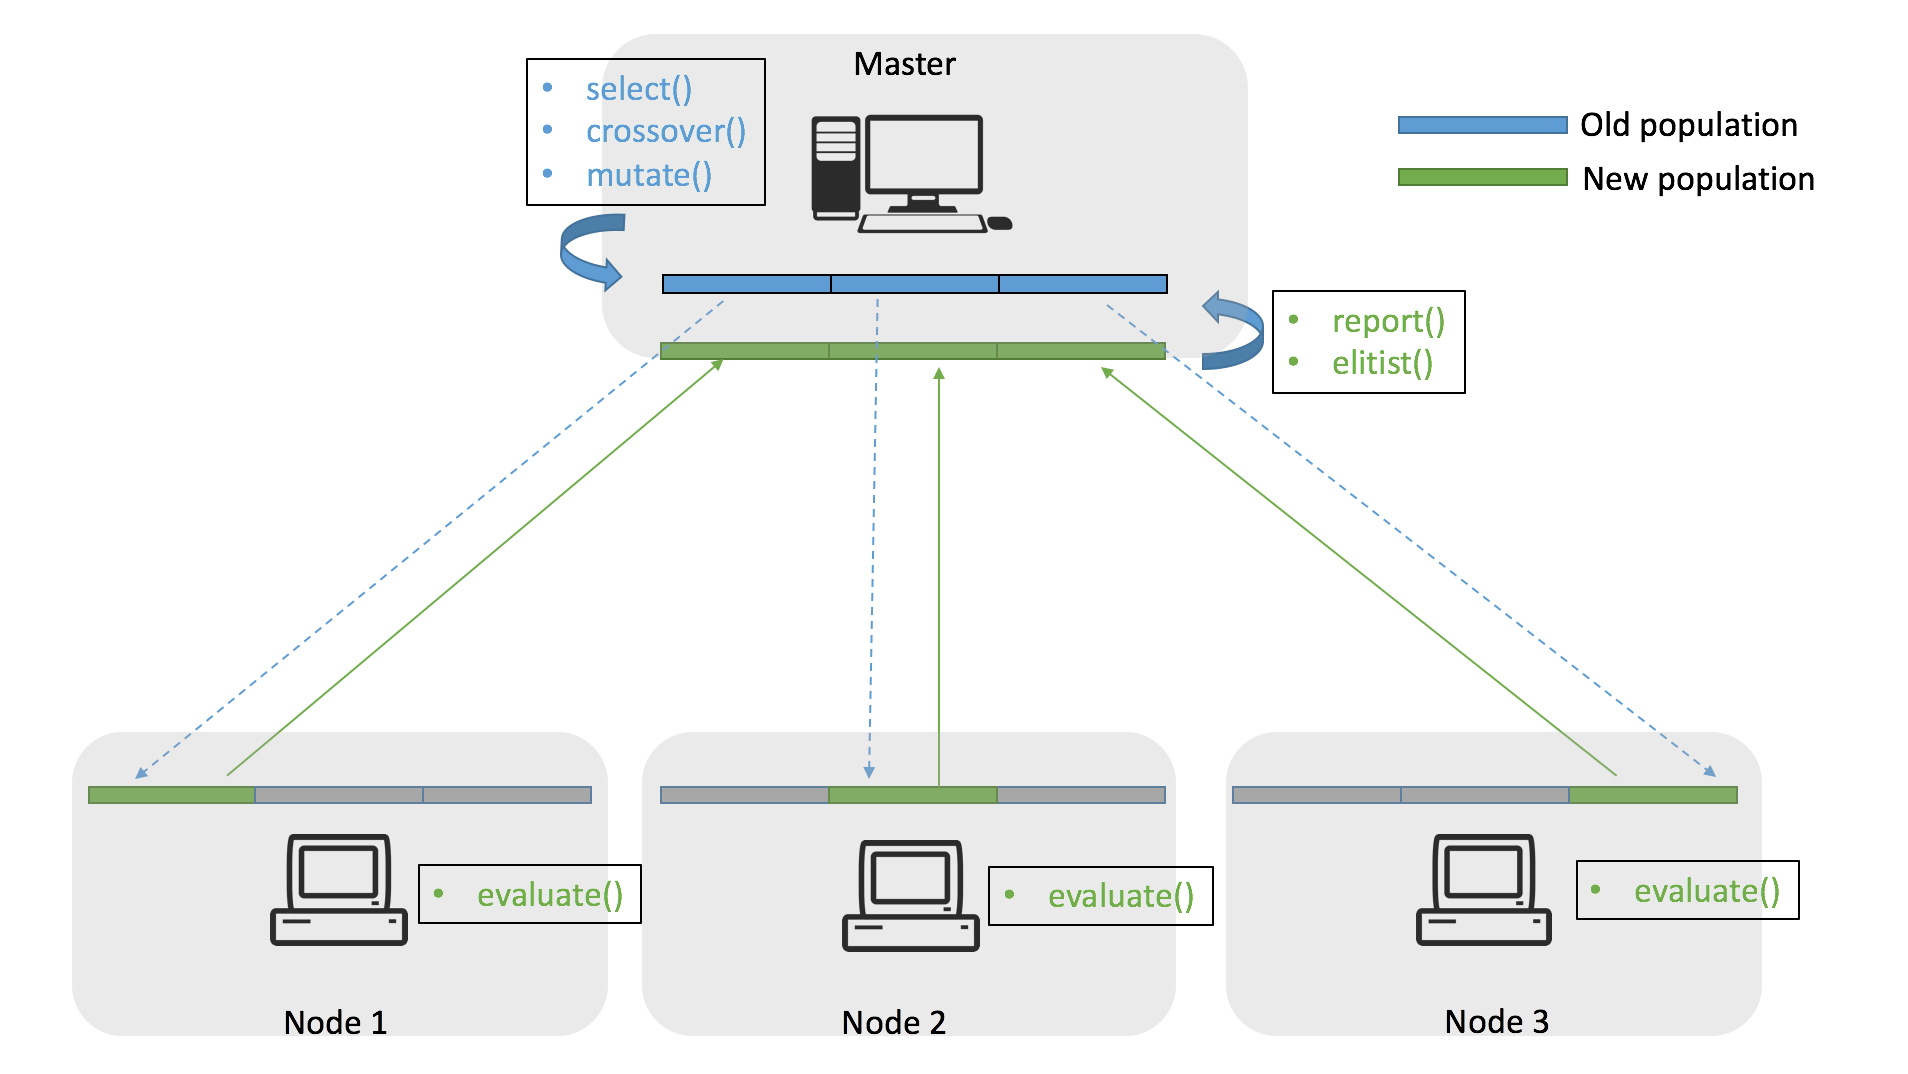
\includegraphics[width= \linewidth]{figs/pga_model_v1.png}
    \caption{PGA v1 model}
     \label{fig:pga_model_v1}
\end{figure}

For each generation, the master\_process() is responsible for performing selection, crossover and mutation operation on entire population ,  dividing population among all available nodes, updating all nodes with their parts of current population, collecting evaluated fitness values from each nodes, evaluate the best member for that generation, report and perform elitist operation on entire population. Where slave process is only responsible to receive a subset of population from master, evaluate their fitness values, send them back to master.  Figure \ref{fig:pga_model_v1} shows the master and slave data decomposition and the GA operation they perform on the population data depends on their role.

\begin{lstlisting}[language=C, caption={Master and slave pr}, label={lst:pga_mpi_main}]
ierr = MPI_Init(&argc, &argv);
ierr = MPI_Comm_size(MPI_COMM_WORLD, &numNodes); // How many nodes
ierr = MPI_Comm_rank(MPI_COMM_WORLD, &myId); // My Rank ID
    
if(myId == MASTER_ID) // Master Process
{
      master_process(filename, seed, mpi_genotype, nodes_data, start);
}
else // Slave processes
{  
    slave_process(seed, mpi_genotype, nodes_data);
}
\end{lstlisting}

\subsubsection{Master process}
In Listing \ref{lst:pga_master_process} parts of the master\_process() procedure is shown. After initialising the initial population master starts performing GA operation on them(lines 3-6). On lines 9-14 it starts sending subset of population to each nodes using MPI\_Send() routine. As we shall see in Listing \ref{lst:pga_slave_process} there is a corresponding MPI\_Recv routine call (line 2) invoked by the slave process. Master then evaluate it's own parts the population subset (line 17). On lines 20-25 master starts to gather the parts of population which have their fitness value calculated by the slave nodes. Then on line 27 master perform elitist() operation using entire population.

\begin{lstlisting}[language=C, caption={The master\_process() procedure.}, label={lst:pga_master_process}]
for(int generation = 0; generation < MAXGENS; generation++)
{   
      selector ( seed );
      crossover ( seed );
      mutate ( seed );     
      report(generation);

      int start_index, item_count;
      for(int nodeId = 1; nodeId < numNodes; nodeId++)
      {
          start_index = nodes_data[nodeId][0];
          item_count = nodes_data[nodeId][1];
          MPI_Send(&population[start_index], item_count, mpi_genotype, nodeId, SEND_DATA_TAG, MPI_COMM_WORLD);
        }
        
      /* Evaluate master's parts of the population */
      evaluate(nodes_data[0][0], nodes_data[0][1]);
        
      /* Collect all parts of new population from each node */
      for(int nodeId = 1; nodeId < numNodes; nodeId++)
      {
          start_index = nodes_data[nodeId][0];
          item_count = nodes_data[nodeId][1];
          MPI_Recv(&population[start_index], item_count, mpi_genotype, nodeId, RETN_DATA_TAG, MPI_COMM_WORLD, &status);
       }
                
      elitist();
}
\end{lstlisting}

\subsubsection{Slave process}
As we can see in Listing \ref{lst:pga_slave_process} the slave process starts with a MPI\_Recv() call on line 4. After receiving the parts for the population slave process perform evaluate() using its own starting index and row count on line 7. When the fitness evaluation is done it start to send the population part to master process by calling MPI\_Send() routine.


\begin{lstlisting}[language=C, caption={The slave\_process() procedure.}, label={lst:pga_slave_process}]
for(int generation = 0; generation < MAXGENS; generation++)
{
    /* Get a subset of population from master */
    ierr = MPI_Recv(&population[my_start], row_count, mpi_genotype, MASTER_ID, SEND_DATA_TAG, MPI_COMM_WORLD, &status);
        
    /* Perform fitness evaluation */
    evaluate (my_start, row_count);
        
    /* Send evaluated population to master */
    MPI_Send(&population[my_start], row_count, mpi_genotype, MASTER_ID, RETN_DATA_TAG, MPI_COMM_WORLD);
}
\end{lstlisting}


\subsection{PGA v2}
\subsubsection{Performance issue with PGA v1}
The first implementation of Master-slave GA as in PGA v1 distribute evaluation of fitness function among several slave processors while master executes the GA operations(selection, crossover and mutation). This implementation explore the search space in exactly same manner as a serial GA and follows exactly the same simple GA design guidelines. It is thought to be the case that, this implementation of master-slave parallel GA results in significant improvement in performance. However, as we shall see in Chapter \ref{empirical} when empirical studies were carried out the actual performance gains seemed to be worse than the serial GA. This is perhaps for the frequent MPI communication overhead that required in each generation for evaluating fitness values back and forth to the master and slave nodes. The execution time time of master-slave GAs have two components; the time used for communication between nodes and the time used in computation. So, the other reason is, master is responsible for performing all GA operations on entire population while slave nodes are mostly sitting idle during this time. With this approach slave nodes are under utilised where master node has a lot of workload 

So, in this version of PGA we tried to leverage some of the GA operations as well as evaluating fitness values to the slave nodes. The movements of population data and node specific GA operations are depicted in Figure \ref{fig:pga_model_v2}.

\begin{figure}[!htb]
        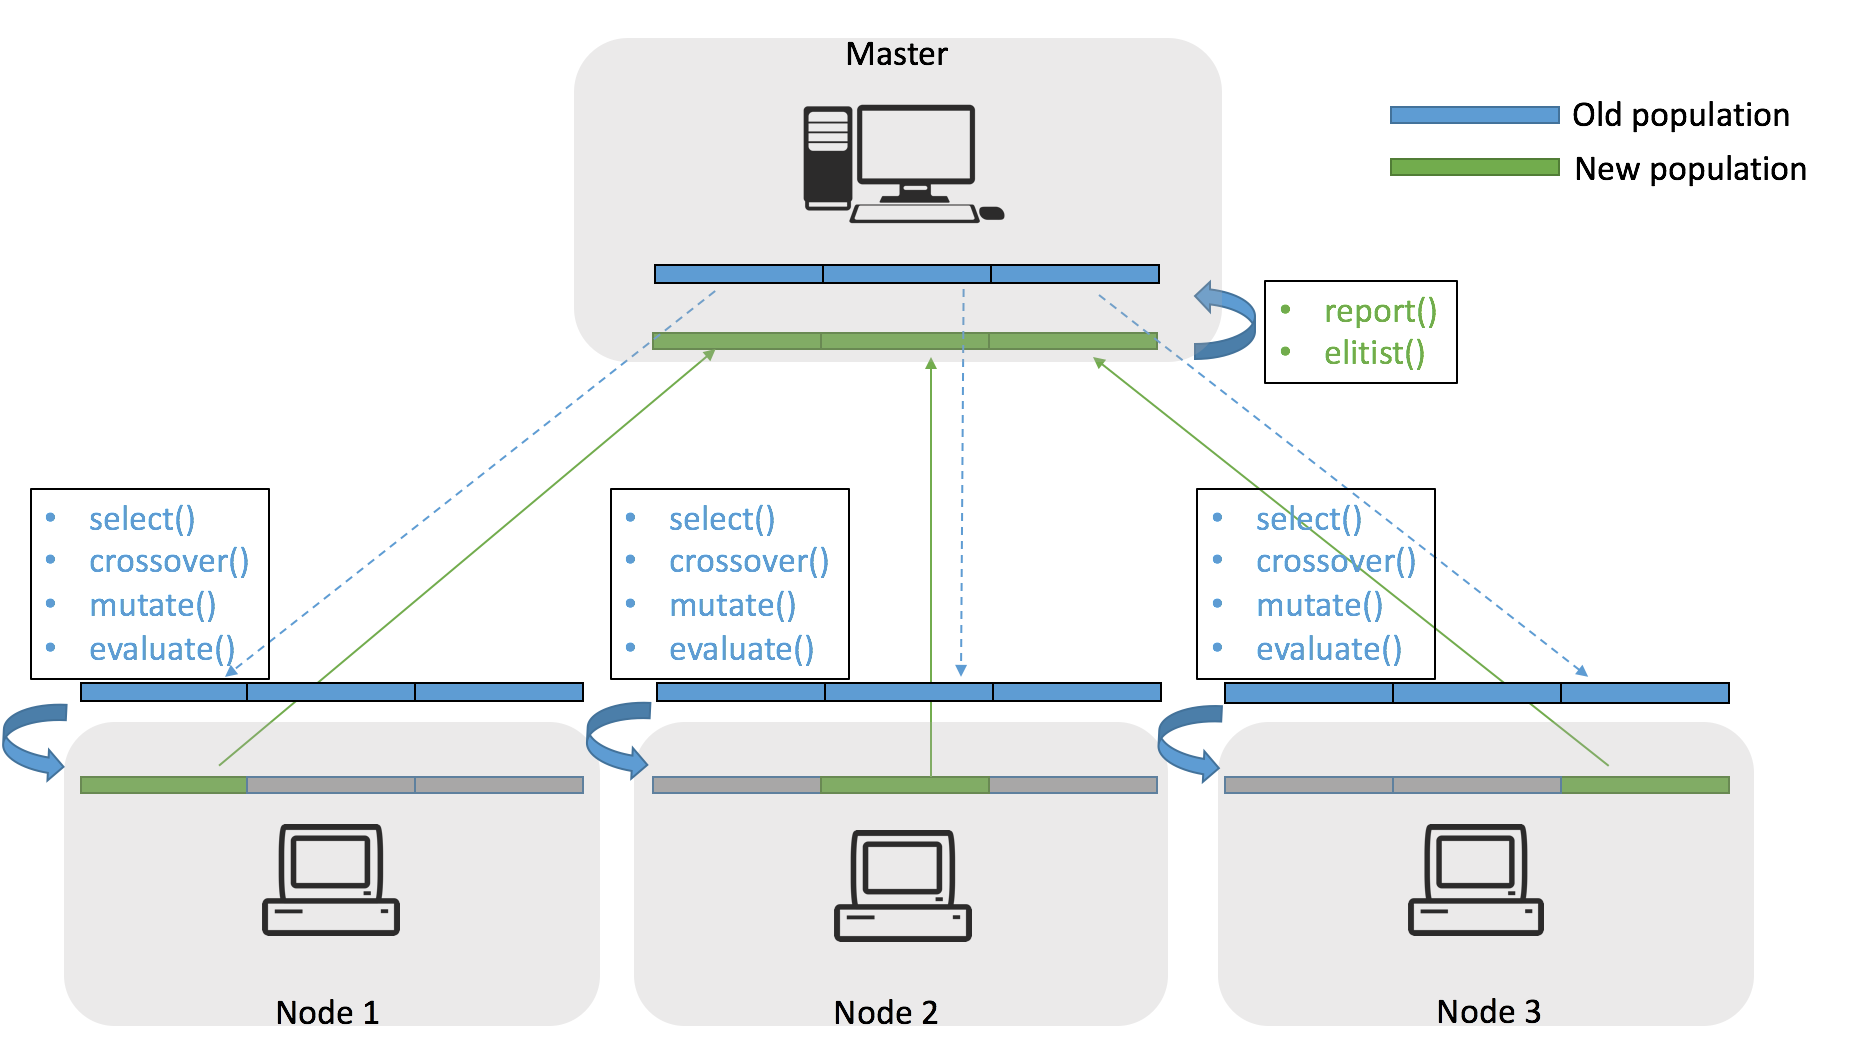
\includegraphics[width= \linewidth]{figs/pga_model_v2.png}
    \caption{PGA v2 model}
     \label{fig:pga_model_v2}
\end{figure}

\subsubsection{Using MPI Broadcast instead of explicit MPI Send/Recv}
To reduce communication overhead MPI collective routine \textbf{MPI\_Bcast()} is used by replacing  explicit \textbf{MPI\_Send() and MPI\_Recv()}. To ensure proper synchronisation among all nodes in the cluster the \textbf{MPI\_Barrier()} is called. When a process calls MPI\_Barrier(), it waits until all of the nodes also call this procedure.

Some part of this implementation is shown in Listing \ref{lst:pga_procedures}. On lines 5-9 master node initialises initial population and perform first elitist operation(keep\_the\_best( )). Slave nodes wait for these operation to complete because of MPI\_Barrier() call on line 12. On line 15 entire population is broadcasted with MPI\_Broadcast() call followed by another call to MPI\_Barrier().  On lines 20-21 all nodes determine their own data partition information. Then all nodes perform GA operations and evaluate the fitness values for the subpopulation(lines 22-27). On lines 32-36 each node then broadcasts its part of the population data. This followed by another synchronisation on line 38 before master node call the elitist() operation on entire population on line 43.

\begin{lstlisting}[language=C, caption={PGA v2 main() procedures.}, label={lst:pga_procedures}]
ierr = MPI_Comm_size(MPI_COMM_WORLD, &numNodes); // How many nodes
ierr = MPI_Comm_rank(MPI_COMM_WORLD, &myId); // My Rank ID
    
/* Initialise first gen population in master process */   
if(myId == MASTER_ID) // Master Process
{        
      initialize ( filename, seed );
      evaluate (0, POPSIZE );
      keep_the_best ( );
}

MPI_Barrier(MPI_COMM_WORLD);
   
/* Broadcast entire first generation from master process */
MPI_Bcast(population, POPSIZE + 1, mpi_genotype, MASTER_ID, MPI_COMM_WORLD);
   
MPI_Barrier(MPI_COMM_WORLD);
 
/* Each process does GA ops here on individual data parts */ 
int my_start = nodes_data[myId][0];
int row_count = nodes_data[myId][1];
for ( generation = 0; generation < MAXGENS; generation++ )
{      
     node_selector (my_start, row_count, seed );
     crossover ( seed );
     node_mutate ( my_start, row_count,seed );   
     evaluate (my_start, row_count);
         
       /* Sync message - 3 */
      MPI_Barrier(MPI_COMM_WORLD);
        
      for(int i = 0; i < numNodes; i++)
      {
          MPI_Bcast(&population[nodes_data[i][0]], nodes_data[i][1], mpi_genotype, i, MPI_COMM_WORLD);
          MPI_Barrier(MPI_COMM_WORLD);
      }
        
      MPI_Barrier(MPI_COMM_WORLD);
        
      if(myId == MASTER_ID) // Master Process
      {
          report(generation);
          elitist ( );
      }
        
      MPI_Barrier(MPI_COMM_WORLD);
}
\end{lstlisting}

\subsection{PGA v3}

\subsubsection{Running Time Analysis of node\_selector() Procedure}
\label{pga_runtime_analysis}
During empirical study of program running time, with PGA v2 we noticed some performance gain when number of processors are increased for smaller population size(5000). We also noticed there is a drop of speedup when population size is increased.

After a some investigation into this problem it was identified that the running time of \textbf{selector()} procedure is contributing for this unexpected result. The Listing \ref{lst:pga_select} parts of this procedure where we can see there is a nested for loop. The outer loop(line 2) on line has a range of \textit{$(0, n/p)$} and the inner loop(line 11) has a range of  \textit{$(0, p)$} where  \textit{n} is the population size and \textit{p} is number of processors. Thus this function has a running time complexity of $\mathcal{O}(n/p * n)$ which is essentially $\mathcal{O}(n^2)$.

Since, all nodes are executing this node\_selector() procedure using entire global population, the total running time is directly dependent upon the slowest node/processor in the cluster plus communication overheard for each generation cycles.


\begin{lstlisting}[language=C, caption={node\_select() procedure.}, label={lst:pga_select}]
/* Select survivors using cumulative fitness. */ 
for ( i = my_start; i < ends; i++ )
{ 
    p = r8_uniform_ab ( a, b, seed );
    if ( p < population[0].cfitness )
    {
        newpopulation[i] = population[0];   
    }
    else
    {
        for ( j = 0; j < POPSIZE; j++ )
        {
            if ( population[j].cfitness <= p && p < population[j+1].cfitness )
            {
                newpopulation[i] = population[j+1];
            }
        }
    }
}
\end{lstlisting}


\subsubsection{Limiting Selection to Partial Population}
Based on the analysis discussed above, in this implementation the \textbf{selector()} procedure is modified so that the selection is done using nodes local subpopulation. Thus this would result in running time complexity of $\mathcal{O}((n/p) * (n/p))$ i.e . $\mathcal{O}((n/p)^2)$ Theoretically, if we could add more nodes i.e. processors we could reduce the affect of population size increases for this procedure proportionally. We know that number of processor cannot always be matched with population size increases but for a reasonably large population size (not infinite), adding in extra nodes can reduce the running time complexity of this function significantly. Figure \ref{fig:pga_model_v3} shows the data partition and GA operation for master and slave nodes. All GA operation including selection is done on subpopulation.

\begin{figure}[!htb]
        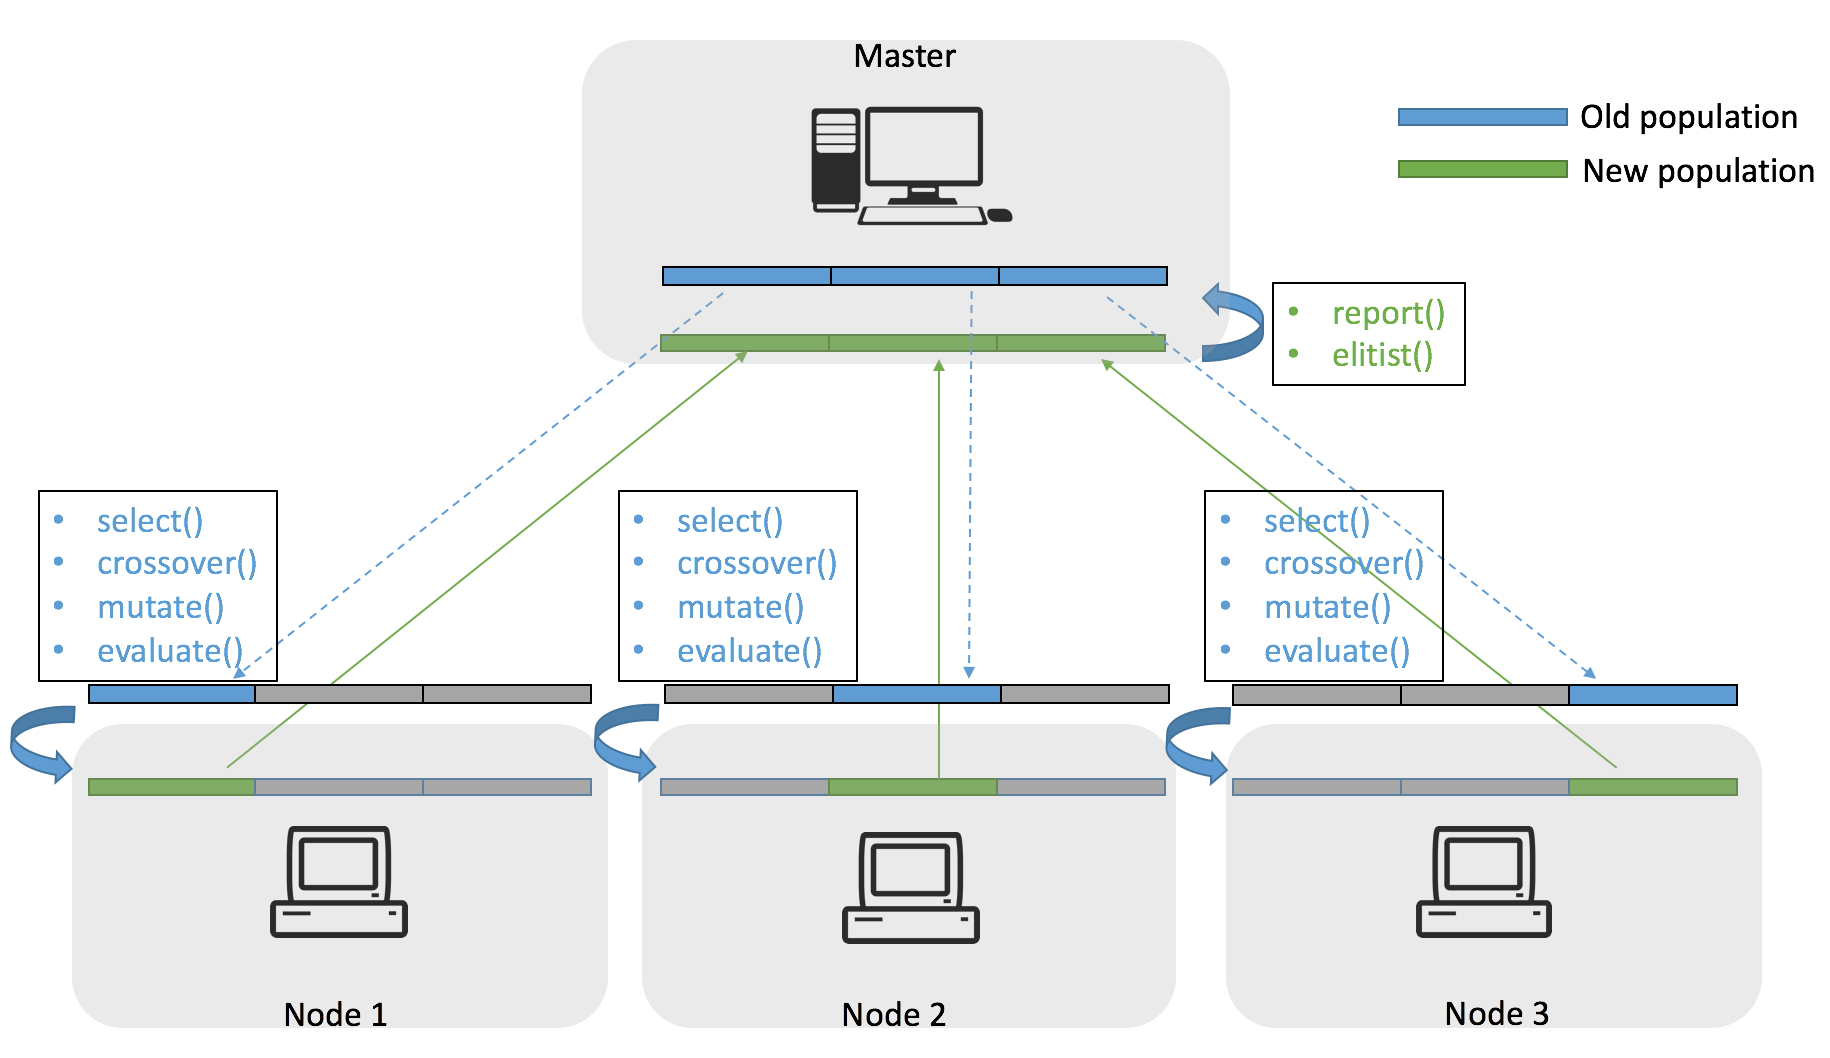
\includegraphics[width= \linewidth]{figs/pga_model_v3.png}
    \caption{PGA v3 model}
     \label{fig:pga_model_v3}
\end{figure}

Changes to the selector functions are shown in Listing \ref{lst:pga_select_changes} where the range inner for loop at line 10 is limited for the local subpopulation only which gives a range of \textit{$(0, n/p)$}.

\begin{lstlisting}[language=C, caption={Changes made in node\_select() procedures.}, label={lst:pga_select_changes}]
for ( i = my_start; i < ends; i++ )
{ 
    p = r8_uniform_ab ( a, b, seed );
    if ( p < population[my_start].cfitness )
    {
        newpopulation[i] = population[my_start];      
    }
    else
    {
        for ( j = my_start; j < ends; j++ )
        { 
            if ( population[j].cfitness <= p && p < population[j+1].cfitness )
            {
                newpopulation[i] = population[j+1];
            }
        }
    }
}
\end{lstlisting}

\subsection{Issues with Serialising Dynamic Data}
The SGA implementation allows population size, number of variables in a chromosome and number of generation can only be modified at compile time. To carry out the experiments we needed the PGA accept these parameters at runtime. So, an attempt was made to change these parameters at runtime with command line arguments. After a week of trials, this attempt was unsuccessful because of a number of reasons which are discussed here. Part of the problem was due to the data structure chosen to represent the chromosome which contains three static array members. The length of these arrays are defined at compile time. Population are initialised inside initialize\(\) procedure (Listing \ref{lst:initialize_proc}). Each individual is initialised with random permissible value. In this trial changes were made to the genotype data structure so that it could be initialised with dynamic arrays using malloc(). Program was compiled normally without any error. But during testing the PGA failed to produce acceptable outcome.

To find the underlying issue GDB was used to debug the problem. During this debugging program was run with a population size of 5. So the best member of a generation is kept  at index 5.
 
It was noticed(GDB output - Listing \ref{lst:gdb_output}) that some values of population members were changing unexpectedly. As we can see from the source code given in Appendix \ref{src:sga_proc.cpp} the initialize() procedure only assign initial value for \textbf{lbound}, \textbf{ubound} and \textbf{gene}. In this debugging session, the values of i, j and the best individual(population[5]) was monitored to catch unexpected any change. On line 42 we see that the value of  population[5].gene is 0x626330. But on next step on line 54 this value has changed to 0x3fe197d48c1f329c. We know that the initialize() procedure only assign values for the population member from 0 to (POPSIZE - 1) which is 4 in this run. So, the changes in population[5] is unexpected. It appeared that even though no value was assigned for best individual (which is population[5]), its member's values were changing. After looking more closely, it was noticed that the value that was being assigned to a data member for one individual was appearing inside some other individual's data member. Which means values were being assigned into wrong memory location. This indicated that malloc() for initialising the population array was not correct.


\begin{lstlisting}[style=BashInputStyle, label={lst:gdb_output}]
847 population[j].gene[i] = r8_uniform_ab ( lbound, ubound, seed );
1: population[5] = {fitness = 0, rfitness = 1.6304166312761136e-322, 
_ cfitness = 0, gene = 0x626330}
2: i = 0
3: j = 2
(gdb) 
840 for ( j = 0; j < POPSIZE; j++ )
1: population[5] = {fitness = 0, rfitness = 1.6304166312761136e-322, 
_ cfitness = 4.147546169663503, gene = 0x626330}
2: i = 0
3: j = 2
(gdb) 

.....

840 for ( j = 0; j < POPSIZE; j++ )
1: population[5] = {fitness = 0, rfitness = 1.6304166312761136e-322, 
_ cfitness = 4.147546169663503, gene = 0x626330}
2: i = 1
3: j = 1
(gdb) 
842 population[j].fitness = 0;
1: population[5] = {fitness = 0, rfitness = 1.6304166312761136e-322, 
_ cfitness = 4.147546169663503, gene = 0x626330}
2: i = 1
3: j = 2
(gdb) 
843 population[j].rfitness = 0;
1: population[5] = {fitness = 0, rfitness = 1.6304166312761136e-322, 
_ cfitness = 4.147546169663503, gene = 0x626330}
2: i = 1
3: j = 2
(gdb) 
844 population[j].cfitness = 0;
1: population[5] = {fitness = 0, rfitness = 1.6304166312761136e-322, 
_ cfitness = 4.147546169663503, gene = 0x626330}
2: i = 1
3: j = 2
(gdb) 
847 population[j].gene[i] = r8_uniform_ab ( lbound, ubound, seed );
1: population[5] = {fitness = 0, rfitness = 1.6304166312761136e-322, 
_ cfitness = 4.147546169663503, gene = 0x626330}
2: i = 1
3: j = 2
(gdb) 
840 for ( j = 0; j < POPSIZE; j++ )
1: population[5] = {fitness = 0, rfitness = 1.6304166312761136e-322, 
_ cfitness = 4.147546169663503, gene = 0x3fe197d48c1f329c}
2: i = 1
3: j = 2
(gdb) 
842 population[j].fitness = 0;
1: population[5] = {fitness = 0, rfitness = 1.6304166312761136e-322, 
_ cfitness = 4.147546169663503, gene = 0x3fe197d48c1f329c}
2: i = 1
3: j = 3
\end{lstlisting}

After this discovery, one and half week time was spent on how to allocate memory correctly for the \textbf{genotype} struct. But it seemed quite complicated to do so with three variable length array members in a struct. By researching on Internet about this, it was found that this issue is known as Variable Length Array In Struct(VLAIS). And with further research, some discussions related to this topic was found in Stackoverflow. The suggestions there were indicating that VLAIS is permissible on specific compiler i.e GCC C99 compatible only.  In one discussion posted on Stackoverflow \footnote{http://stackoverflow.com/questions/21804994/using-a-struct-member-as-array-size-in-the-same-struct} related to this topic further suggested that that variable-length arrays in structs is permissible in gcc (and the newest C-standards), but the variable array must always be the last member of the struct (so the compiler knows where all members are). In particular this means:

\begin{enumerate}
	\item There can be only one variable-length array
	\item If the struct is a member of another struct, it has to be the last member of that struct.
\end{enumerate}

Another post \footnote{http://stackoverflow.com/questions/17552312/multiple-flexible-array-in-a-struct-in-c} also suggested that it is not possible to have more than one flexible-array member in a struct.

There is no clear information whether mpic++ compiler has support for this feature of gcc too or not. The alternative solution to this problem would be to replace struct data structure with combination of C++ objects and vectors. Since this would have involved making a considerable changes to actual SGA implementation and possibilities of going back to the earlier problem with Object-oriented GA, a decision was made to leave these parameters to be defined at compile time.

\section{Testing}
To ensure the Parallel Genetic Algorithms implementations are producing expected outcome there is no alternative but to carry out testing. These tests were performed to validate the correctness of PGA implementation. We wanted to see if the output of the PGA program is consistent with the output of original SGA program using same parameters values and random seed.

\subsection{Test Configuration}
\label{test_config}
The common parameter values shown in Table \ref{tbl:test_params} are used for all testing both SGA and PGA programs.

\begin{table}[]
\centering
\caption{Parameters alues used with test cases.}
\label{tbl:test_params}
\begin{tabular}{|l|l|l|}
\hline
\textbf{Parameter}  & \textbf{Description }                        & \textbf{Value}     \\ \hline
POPSIZE    & Population Size                     & 5000      \\ \hline
MAXGENS    & Number of Generation                & 100       \\ \hline
NVARS      & Number of variables in a Chromosome & 3         \\ \hline
PXOVER     & Probability of Crossover            & 0.8       \\ \hline
PMUTATION  & Probability of Mutation             & 0.15      \\ \hline
FITNESS\_F & Fitness function (F8: Griewank)                   & F8        \\ \hline
SEED       & Random value generator seed         & 123456789 \\ \hline
Genome Encoding       & Encoding scheme for genome representaion         & Real value Encoding \\ \hline
\end{tabular}
\end{table}

As the original SGA was implemented with Real-value encoding scheme for genome representation the range of these values are given using a input file. For this test configuration with 3 genome per chromosome the permissible values are given as listed in Table \ref{tbl:genome_range}.

\begin{table}[]
\centering
\caption{Genome value range for 3 variables Griewank function}
\label{tbl:genome_range}
\begin{tabular}{|l|l|}
\hline
\textbf{Lower} & \textbf{Upper} \\ \hline
-512.0           & 511.0            \\ \hline
-512.0           & 511.0            \\ \hline
-512.0           & 511.0            \\ \hline
\end{tabular}
\end{table}

As discussed in section \ref{beowulf:process_manager} the hosts information entries shown in Listing \ref{lst:config_hydra} were added for Hydra (MPI Process Manager). The entry at line 1 is master node's hostname. Which means master node also is acting as a compute node in the cluster.

\begin{lstlisting}[style=BashInputStyle, label={lst:config_hydra}, caption={The hosts file configuration for Hydra.}]
padma:2
meghna:2
jamuna:2
\end{lstlisting} 

The PGA program was run by using following command:
\begin{lstlisting}[style=BashInputStyle, label={lst:run_mpi}]
$mpiexec -f ~/hosts -n 6 ./pga
\end{lstlisting}
The command \textbf{mpiexec} takes in parameter \textbf{-f} for the hosts file name and \textbf{-n} for  the number of processes that needs to be created in the cluster. The example shown above will launch 6 process that will run the executable binary \textbf{pga}.

\textbf{All tests results shown in this section are carried out in Hardware based Beowulf} system not in simulated cluster.

\subsection{Tests Outcome}
The GA programs output for the SGA, PGA v1, PGA v2 and PGA v3 are shown below. As these tests were run with a generation size if 100 the full output is not shown to save space. Instead, outputs are shown into two split images "Top part" and "Bottom part" of the screen capture that convey most important information. We are assuming the original SGA program is producing a correct output. Then the subsequent 3 PGA programs outputs are compared against SGA's output to validate and analyse each PGA implementation. 

\subsubsection{SGA Output}

Figures \ref{fig:test_sga_top} and \ref{fig:test_sga_bottom} shows the output of original SGA program compiled with the parameter configuration discussed in section \ref{test_config}.

\begin{figure}[!htb]
	\center
        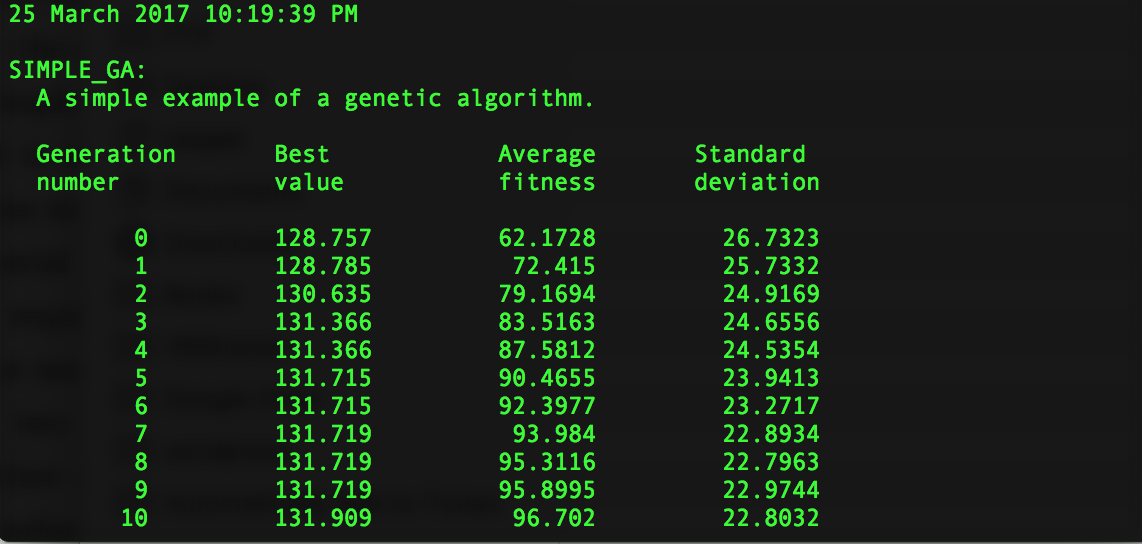
\includegraphics[width= \linewidth]{figs/tests/sga_top.png}
    \caption{SGA output - Top part}
     \label{fig:test_sga_top}
\end{figure}

\begin{figure}[!htb]
	\center
        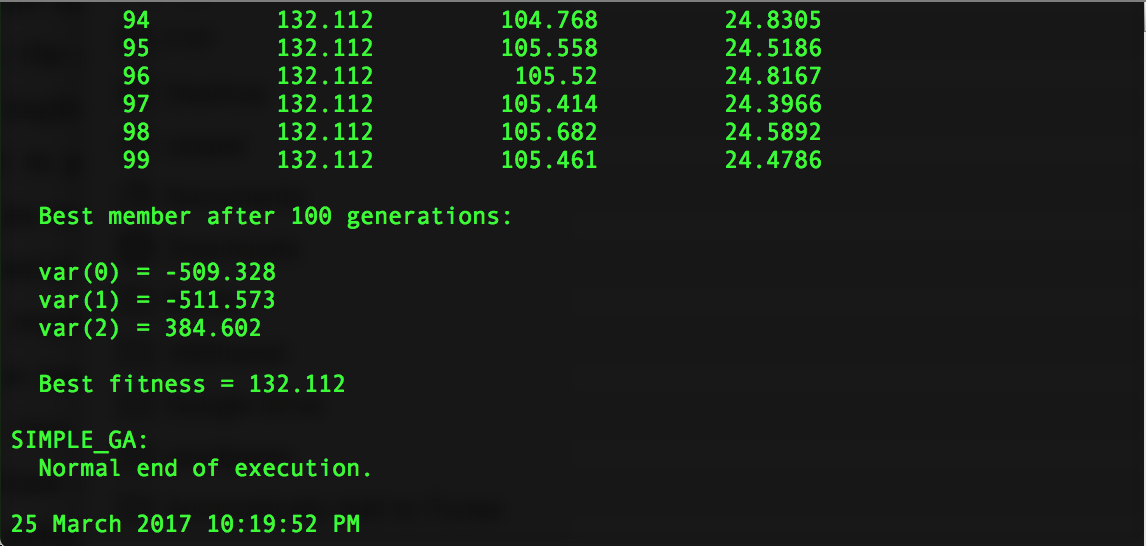
\includegraphics[width= \linewidth]{figs/tests/sga_bottom.png}
    \caption{SGA output - Bottom part}
     \label{fig:test_sga_bottom}
\end{figure}

\subsubsection{PGA v1 Output}

Figures \ref{fig:test_pga_top} and \ref{fig:test_pga_bottom} shows the output of original PGA v1 compiled with the parameter configuration discussed in section \ref{test_config}.

\begin{figure}[!htb]
	\center
        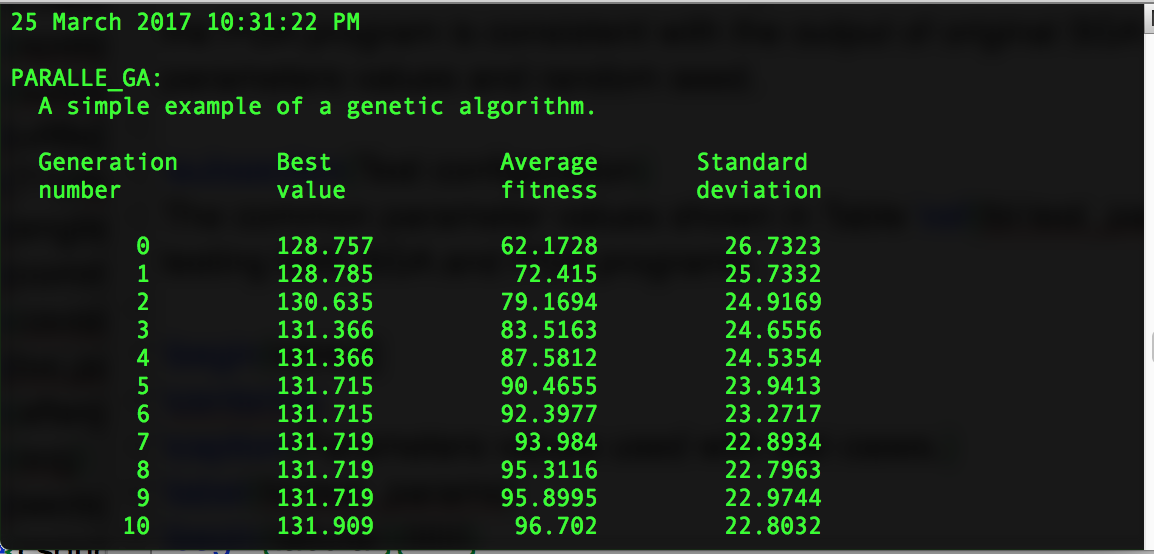
\includegraphics[width= \linewidth]{figs/tests/pga_top.png}
    \caption{PGA v1 output - Top part}
     \label{fig:test_pga_top}
\end{figure}

\begin{figure}[!htb]
	\center
        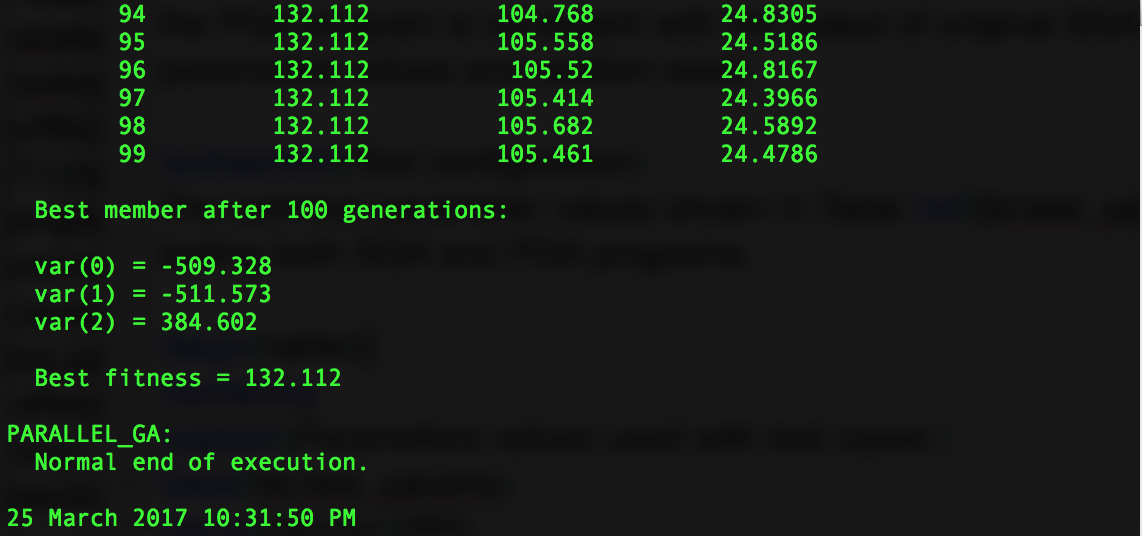
\includegraphics[width= \linewidth]{figs/tests/pga_bottom.png}
    \caption{PGA v2 output - Bottom part}
     \label{fig:test_pga_bottom}
\end{figure}

\subsubsection{PGA v2 Output}

Figures \ref{fig:test_pgav2_top} and \ref{fig:test_pgav2_bottom} shows the output of original PGA v2 compiled with the parameter configuration discussed in section \ref{test_config}.

\begin{figure}[!htb]
	\center
        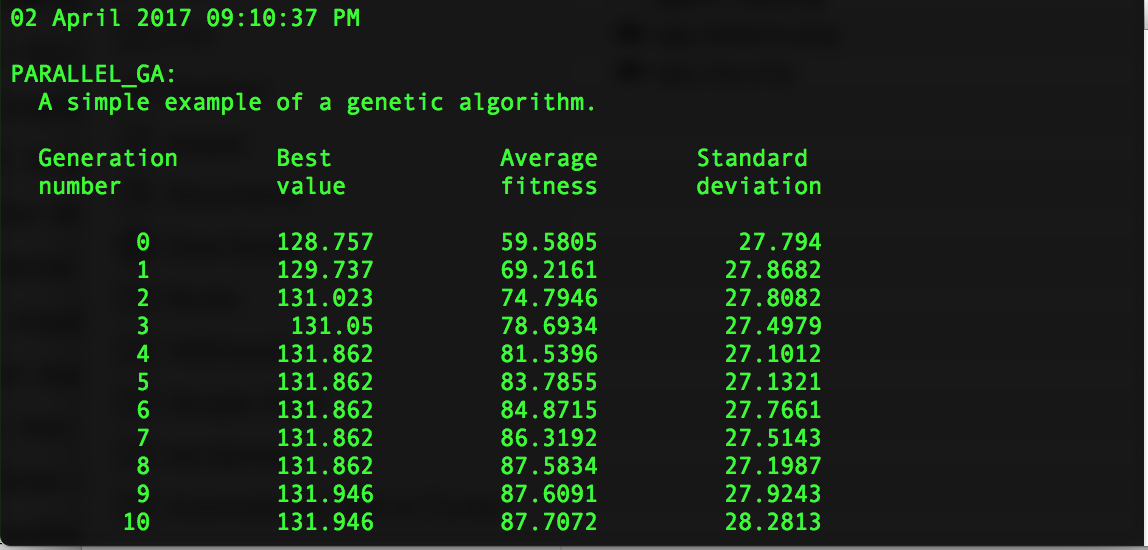
\includegraphics[width= \linewidth]{figs/tests/pgav2_top.png}
    \caption{PGA v1 output - Top part}
     \label{fig:test_pgav2_top}
\end{figure}

\begin{figure}[!htb]
	\center
        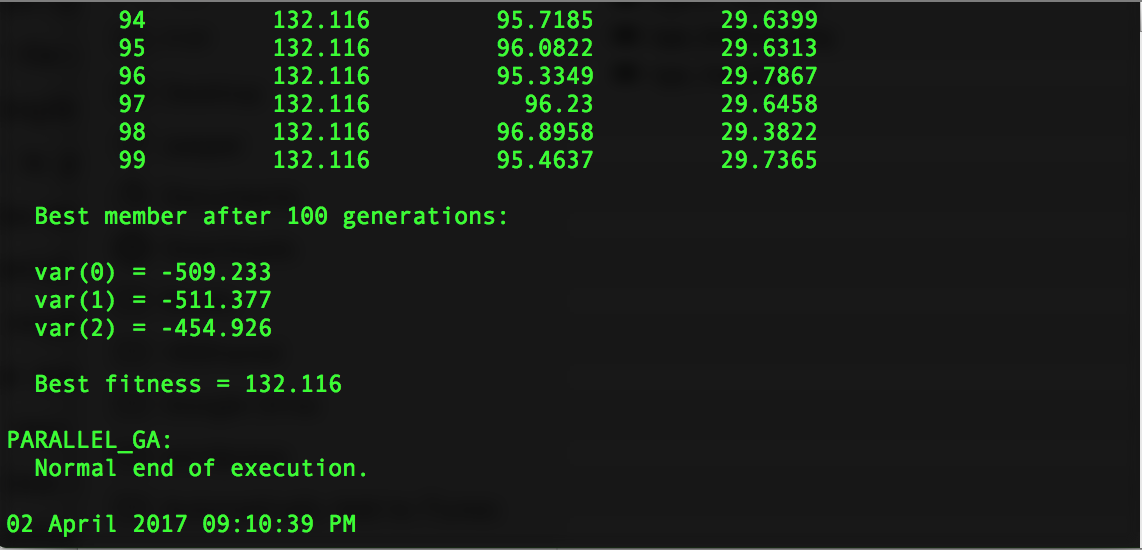
\includegraphics[width= \linewidth]{figs/tests/pgav2_bottom.png}
    \caption{PGA v2 output - Bottom part}
     \label{fig:test_pgav2_bottom}
\end{figure}

\subsubsection{PGA v3 Output}

Figures \ref{fig:test_pgav3_top} and \ref{fig:test_pgav3_bottom} shows the output of original PGA v3 compiled with the parameter configuration discussed in section \ref{test_config}.

\begin{figure}[!htb]
	\center
        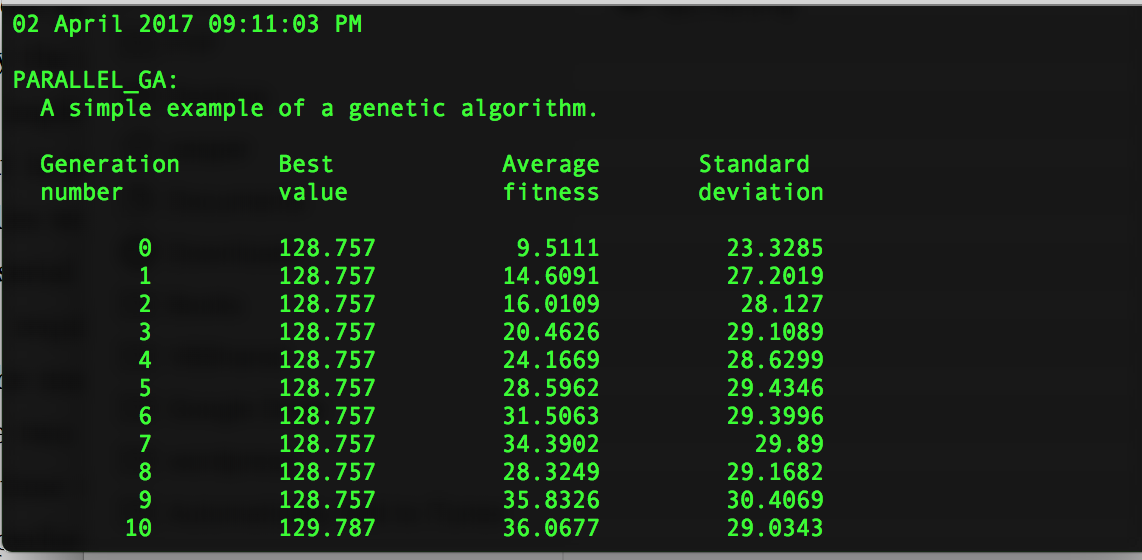
\includegraphics[width= \linewidth]{figs/tests/pgav3_top.png}
    \caption{PGA v3 output - Top part}
     \label{fig:test_pgav3_top}
\end{figure}

\begin{figure}[!htb]
	\center
        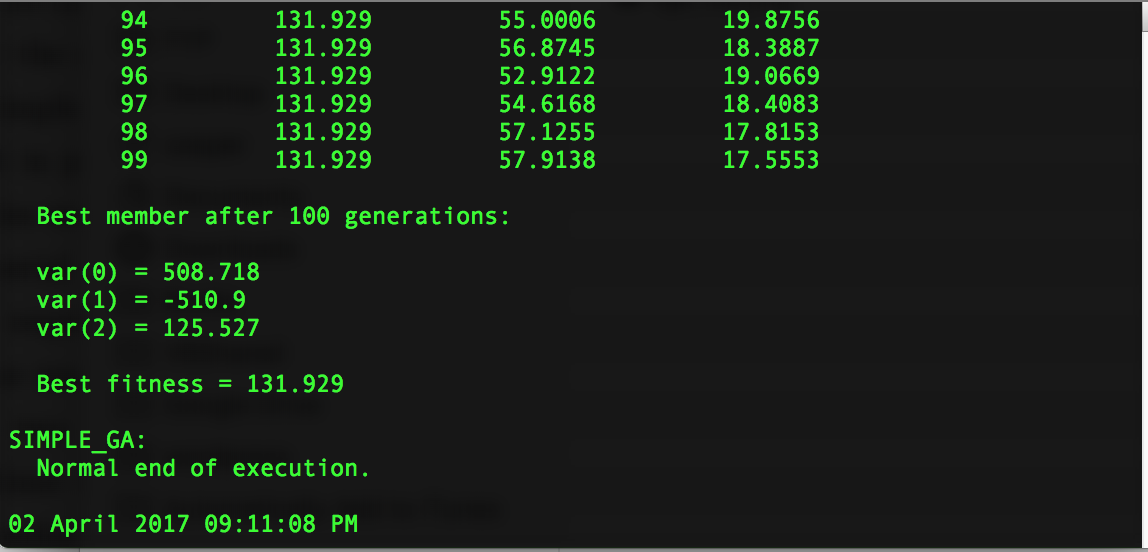
\includegraphics[width= \linewidth]{figs/tests/pgav3_bottom.png}
    \caption{PGA v3 output - Bottom part}
     \label{fig:test_pgav3_bottom}
\end{figure}

 



\section{Discussion}
The Beowulf implementation required a further steps for administrative tasks such and allowing remote access using vncserver, configuring ddns so that the system is accessible while not working from home. Since, the development needed the cluster setup to compile and and run MPI program the Integrated Development Environment set was also configured so that it able to use the remote cluster infrastructure. The necessary details are omitted here because of space constraint and they are not the main focus point of this project.

As described in previous section in this chapter, in this project we only explored one model of parallel GA which is master-slave model. In conjunction with the tests results and experiments shown in next chapter we see that pure master-slave model of PGA(PGA v1) did not give us any speed up at all, which is understandable since the communication overhead for message-passing actually more costly than actual computation done by multiple nodes. With PGA v2 where we changed the algorithm to utilise all nodes to do the GA operations instead of just computing fitness value we started to see speedup improvements. But this gains were not as much as expected. Lastly, in PGA v3 we limited the selection space to the subpopulation that a node operates on. This implementation gives us a good speedup gains. However, as we can see from the tests result of PGA v3 the actual outcome of GA is slightly worse than that of original SGA. That is because PGA v3 is close to a distributed PGA model as discussed in Section 2.5.3 without any migration policy. Next logical step of this project would be to implement a distributed model of PGA with a migration policy. Due to the time constraint of this project we needed to stop at the PGA v3.

\chapter{Empirical studies}
\label{empirical}

\section{Introduction}
%=============================
In this chapter the runtime of three Parallel GA(PGA) implementations (discussed in previous chapter) are compared against the sequential GA implementation. Each implementation is compared and contrasted with SGA. We focused this study on to observe the program runtime by varying number of processes and by varying the population size. These experiments were carried out on a physical Beowulf cluster setup as described in Section \ref{test_config} with test configurations shown in Section \ref{test_config}. Results may vary using other cluster configuration.


Even though we kept the free-parameter's values consistent throughout the experiments there are other constraints on which we do not have any explicit control to fine tune them. This constraints include Linux schedular (which runs other system daemons and services), and network system overhead. Extra care was taken to ensure no other programs were running during the experiments and network activities were minimum. To further validate our experiments data  statistical method of confidence interval were used. 

In statistics, a confidence interval (CI) is a type of interval estimation of a random variable (in this experiment which is the program run time). It is an observed interval (i.e. calculated from the observations). In principle this interval is different from sample to sample, that potentially includes the unobservable true parameter of interest. How frequently the observed interval contains the true parameter if the experiment is repeated is called the confidence level. If confidence intervals are constructed in separate experiments on the same population following the same process, the proportion of such intervals that contain the true value of the parameter will match the given confidence level\citep{cox1979theoretical}. Whereas two-sided confidence limits form a confidence interval, and one-sided limits are referred to as lower/upper confidence bounds (or limits).

All of the sample runtime data gathered here are averaged from 20 runs. Due to time constraint sample size is kept 20 which means we run each program for 20 times and recorded the time taken from start to finish for each run. To calculate CI the average \textbf{$ \bar{x} $ } and standard deviation \textbf{$ \delta $} is calculated of these 20 data set. Then the CI is calculated using following formula where \textbf{$z = 1.96 $} for 95\% CI:
\[
	Upper Limit = \bar{x} + z (\delta/\sqrt{20})
\]
\[
	Lower Limit = \bar{x} - z (\delta/\sqrt{20})
\]

Table \ref{tab:emp_table_1} shows the data of average running time for all three implementation of PGA using a population size 5000 with their upper and lower bound with 95\% confidence level. Which means that 95\% of time time the true value of the program runtime is within our confidence interval. After any particular sample is taken, given that exactly same configuration were used, the program runtime should be within these intervals shown in the Table \ref{tab:emp_table_1} 95\% of the time.


\begin{table}[!htb]
\centering
\caption{A sample runs using population size of 5000 to determine average runtime(seconds) for PGA v1, PGA v2 and PGA v3.}
\label{tab:emp_table_1}
\begin{tabular}{|l|l|l|l|}
\hline
RUN                & PGA v1   & PGA v2  & PGA v3  \\ \hline
0                  & 14.8262 & 5.0441 & 1.7067 \\ \hline
1                  & 14.7368 & 5.0157 & 1.9845 \\ \hline
2                  & 15.0571 & 4.9169 & 1.7116 \\ \hline
3                  & 15.0404 & 4.9911 & 1.6933 \\ \hline
4                  & 16.2858 & 4.9056 & 1.6935 \\ \hline
5                  & 14.5847 & 5.0745 & 1.7016 \\ \hline
6                  & 14.7812 & 5.0515 & 1.6980 \\ \hline
7                  & 15.4188 & 5.0403 & 1.7069 \\ \hline
8                  & 16.4531 & 4.9878 & 1.6974 \\ \hline
9                  & 16.9943 & 4.8959 & 1.7039 \\ \hline
10                 & 15.7324 & 4.9217 & 1.6986 \\ \hline
11                 & 14.4173 & 4.9180 & 1.7055 \\ \hline
12                 & 14.6054 & 5.0879 & 1.7063 \\ \hline
13                 & 14.8513 & 4.9155 & 1.7112 \\ \hline
14                 & 15.4737 & 4.9294 & 1.7024 \\ \hline
15                 & 14.4207 & 5.0595 & 1.6966 \\ \hline
16                 & 16.0418 & 5.0947 & 1.7095 \\ \hline
17                 & 16.8885 & 5.0685 & 1.6873 \\ \hline
18                 & 15.0276 & 4.9684 & 1.7136 \\ \hline
19                 & 16.4414 & 4.9665 & 1.7077 \\ \hline
\multicolumn{4}{|l|}{}                         \\ \hline
Average            & 15.4039 & 4.9927 & 1.7168 \\ \hline
Standard Deviation & 0.8162  & 0.0670 & 0.0618 \\ \hline
CI (95\%)          & 0.3577  & 0.0294 & 0.0271 \\ \hline
\multicolumn{4}{|l|}{}                         \\ \hline
Upper Limit        & 15.7616 & 5.0220 & 1.7439 \\ \hline
Lower Limit        & 15.0462 & 4.9633 & 1.6897 \\ \hline
\end{tabular}
\end{table}


Using this method all data for the experiments listed below were validated. The results shown for these experiments are the average of 20 runs.

\section{Experiments using PGA v1}
%=============================

\subsection{Experiment 1: Varying number of processes}

\subsubsection{Objective}
Comparison of PGA v1 runtime vs. SGA runtime by varying the number of processes the work is distributed for the PGA program to see the speedup gain using a fixed population size 5000.

\begin{table}[H]
\centering
\caption{Experiment 1 data using PGA v1}
\label{tab:pga1_node}
\begin{tabular}{|l|l|l|l|}
\hline
\# Process(es) & SGA     & PGA     & speedup \\ \hline
1        & 12.8789 & 12.8887 & 0.9992  \\ \hline
2        & 12.8789 & 12.8464 & 1.0025  \\ \hline
3        & 12.8789 & 13.1183 & 0.9818  \\ \hline
4        & 12.8789 & 13.1585 & 0.9788  \\ \hline
5        & 12.8789 & 13.4671 & 0.9563  \\ \hline
6        & 12.8789 & 15.3387 & 0.8396  \\ \hline
\end{tabular}
\end{table}

\begin{figure}[H]
\begin{center}
  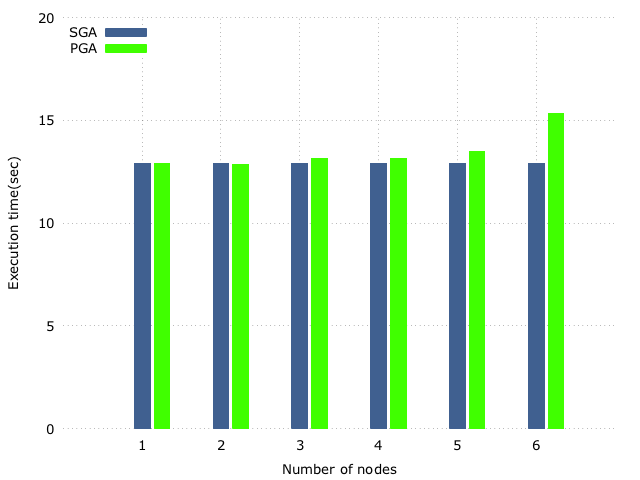
\includegraphics[width=.7 \linewidth]{stats_data_new/graphs/pga_xNodes_hist.png}
  \caption{Experiment 1 - Runtime comparison SGA vs PGA v1.}
  \end{center}\
\end{figure}

\begin{figure}[H]
\begin{center}
  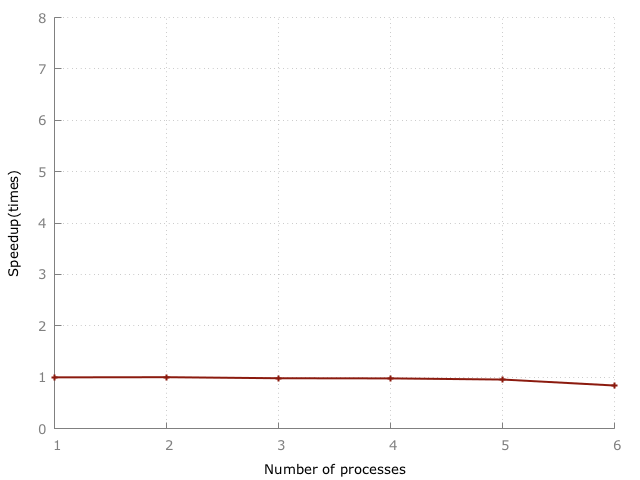
\includegraphics[width=.7 \linewidth]{stats_data_new/graphs/pga_xNodes_line.png}
  \caption{Experiment 1: Speedup graph SGA vs PGA v1.}
  \end{center}\
\end{figure}

\subsubsection{Discussion}
This experiment shows that there is no speedup gain when the number of processes were increased. That is because the communication overhead for MPI increases as the number of processes increases.

\subsection{Experiment 2: Varying population size}

\subsubsection{Objective}
Comparison of PGA v1 runtime vs. SGA runtime by varying the population size using 6 processes for PGA program.

\begin{table}[H]
\centering
\caption{Experiment 2 data using PGA v1}
\label{tab:pga1_pop}
\begin{tabular}{|l|l|l|l|}
\hline
\# population & SGA     & PGA     & speedup \\ \hline
1000          & 0.57    & 0.6827  & 0.835   \\ \hline
2000          & 2.1459  & 2.3018  & 0.9323  \\ \hline
3000          & 4.7258  & 4.9238  & 0.9598  \\ \hline
4000          & 8.2976  & 11.0389 & 0.7517  \\ \hline
5000          & 12.8896 & 15.7361 & 0.8191  \\ \hline
6000          & 18.4622 & 20.249  & 0.9118  \\ \hline
7000          & 25.0535 & 26.8225 & 0.934   \\ \hline
8000          & 32.667  & 36.5315 & 0.8942  \\ \hline
9000          & 41.3425 & 42.1336 & 0.9812  \\ \hline
10000         & 50.8885 & 51.9144 & 0.9802  \\ \hline
\end{tabular}
\end{table}

\begin{figure}[H]
\begin{center}
  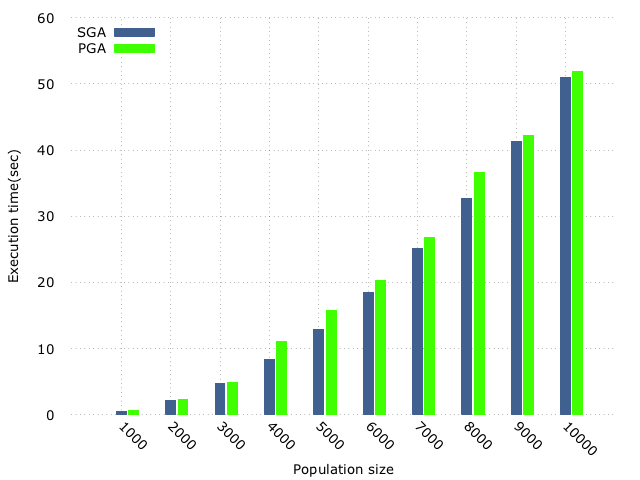
\includegraphics[width=.7 \linewidth]{stats_data_new/graphs/pga_xPop_hist.png}
  \caption{Experiment 2 - Runtime comparison SGA vs. PGA v1.}
  \end{center}\
\end{figure}

\begin{figure}[H]
\begin{center}
  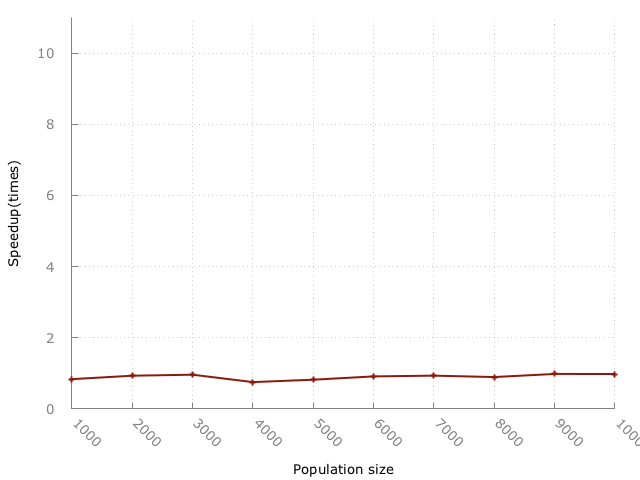
\includegraphics[width=.7 \linewidth]{stats_data_new/graphs/pga_xPop_line.png}
  \caption{Experiment 2 - Speedup graph SGA vs. PGA v1.}
  \end{center}\
\end{figure}

\subsubsection{Discussion}
This experiment shows that there is no speedup gain as the population size were increased either. Again, this shows that the communication overhead for MPI has significant impact of overall runtime of the program. This overhead increases with population size.

\section{Experiments using PGA v2}
%============PGA v2 ==============

\subsection{Experiment 3: Varying number of processes}

\subsubsection{Objective}
Comparison of PGA v2 runtime vs. SGA runtime by varying the number of processes the work is distributed for the PGA program to see the speedup gain using a fixed population size 5000.

\begin{table}[H]
\centering
\caption{Experiment 3 data using PGA v2}
\label{tab:pga2_node}
\begin{tabular}{|l|l|l|l|}
\hline
\# Process(es) & SGA     & PGA     & speedup \\ \hline
1        & 12.8795 & 12.8713 & 1.0006  \\ \hline
2        & 12.8795 & 8.6353  & 1.4915  \\ \hline
3        & 12.8795 & 6.5845  & 1.956   \\ \hline
4        & 12.8795 & 6.7115  & 1.919   \\ \hline
5        & 12.8795 & 5.1471  & 2.5023  \\ \hline
6        & 12.8795 & 5.0748  & 2.538   \\ \hline
\end{tabular}
\end{table}

\begin{figure}[H]
\begin{center}
  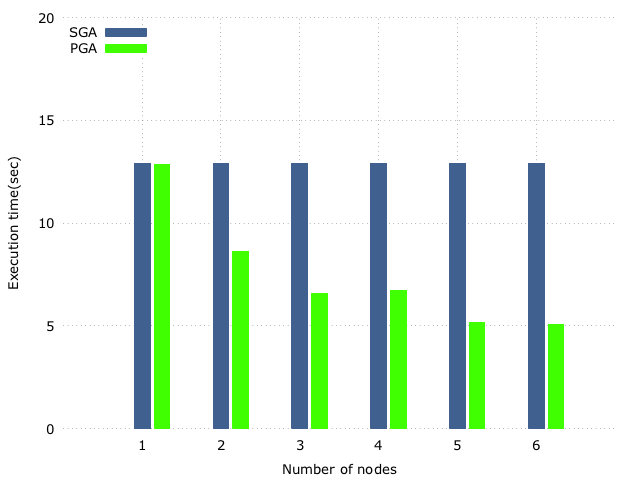
\includegraphics[width=.7 \linewidth]{stats_data_new/graphs/pga_global_xNodes_hist.png}
  \caption{Experiment 3 - Runtime comparison SGA vs. PGA v2.}
  \end{center}\
\end{figure}

\begin{figure}[H]
\begin{center}
  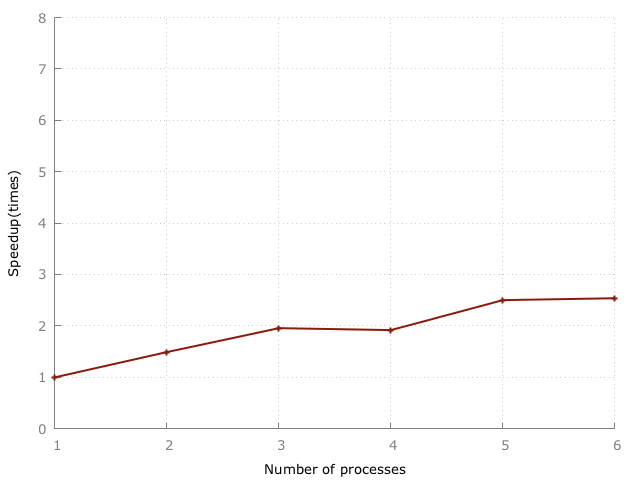
\includegraphics[width=.7 \linewidth]{stats_data_new/graphs/pga_global_xNodes_line.png}
  \caption{Experiment 3 - Speedup graph SGA vs. PGA v2.}
  \end{center}\
\end{figure}

\subsubsection{Discussion}
With this experiment we observed that there is speedup gain with PGA v2 as number of processes increases. However, this gain is much lower than expected with 6 processes given that the MPI collective communication routine were used for this implementation to reduce the communication overhead of PGA v1.

\subsection{Experiment 4: Varying population size}

\subsubsection{Objective}
Comparison of PGA v2 runtime vs. SGA runtime varying the number the population size using 6 processes for PGA program.

\begin{table}[H]
\centering
\caption{Experiment 4 data using PGA v2}
\label{tab:pga2_pop}
\begin{tabular}{|l|l|l|l|}
\hline
\# population & SGA     & PGA     & speedup \\ \hline
1000          & 0.5698  & 0.4957  & 1.1495  \\ \hline
2000          & 2.146   & 1.3006  & 1.65    \\ \hline
3000          & 4.7207  & 2.2022  & 2.1437  \\ \hline
4000          & 8.3287  & 3.4562  & 2.4098  \\ \hline
5000          & 12.8959 & 4.8998  & 2.6319  \\ \hline
6000          & 18.4703 & 7.016   & 2.6326  \\ \hline
7000          & 25.0758 & 21.6343 & 1.1591  \\ \hline
8000          & 32.7814 & 28.134  & 1.1652  \\ \hline
9000          & 41.2779 & 31.5602 & 1.3079  \\ \hline
10000         & 50.9403 & 44.5325 & 1.1439  \\ \hline
\end{tabular}
\end{table}

\begin{figure}[H]
\begin{center}
  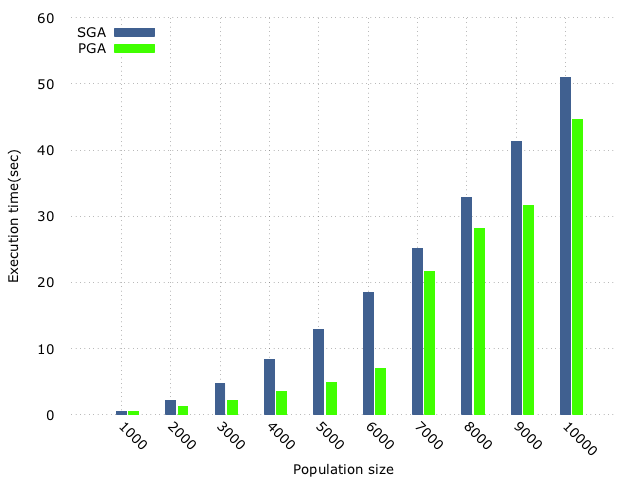
\includegraphics[width=.7 \linewidth]{stats_data_new/graphs/pga_global_xPop_hist.png}
  \caption{Experiment 4 - Runtime comparison SGA vs. PGA v2.}
  \end{center}\
\end{figure}

\begin{figure}[H]
\begin{center}
  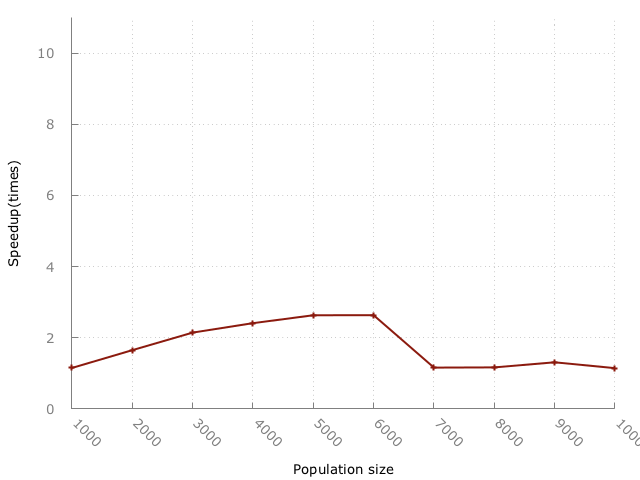
\includegraphics[width=.7 \linewidth]{stats_data_new/graphs/pga_global_xPop_line.png}
  \caption{Experiment 4 - Speedup graph SGA vs PGA v2.}
  \label{fig:exp2_pgav2_graph}
  \end{center}\
\end{figure}

\subsubsection{Discussion}
Result of this experiment is very interesting as we can see from the graph shown in Figure \ref{fig:exp2_pgav2_graph}. In Experiment 3 we saw somewhat of a steady gain in speedup for a fixed population size of 5000. But here we see as population size is increased (after 6000), there is a decrease in speedup. To find out the possible issue that may cause this behaviour, a running time analysis was carried to identify the problem that was discussed in section \ref{pga_runtime_analysis}. It was identified that the selection procedure had a running time complexity of $\mathcal{O}(n^2)$. As population size is increased after a certain threshold (6000 in this experiment) the runtime to this program started to increase rapidly which degraded the overall performance of speedup of this program by parallelising with many processes.

\section{Experiments using PGA v3}
%============PGA v3 ==============

\subsection{Experiment 5: Varying number of processes}

\subsubsection{Objective}
Comparison of PGA v3 runtime vs. SGA runtime varying the number of processes the work is distributed for the PGA program to see the speedup gain using a fixed population size 5000.

\begin{table}[H]
\centering
\caption{Experiment 5 data using PGA v3}
\label{tab:pga3_node}
\begin{tabular}{|l|l|l|l|}
\hline
\# Process(es) & SGA    & PGA     & speedup(SGA/PGA) \\ \hline
1        & 12.878 & 13.3253 & 0.9664           \\ \hline
2        & 12.878 & 3.5889  & 3.5883           \\ \hline
3        & 12.878 & 3.511   & 3.6679           \\ \hline
4        & 12.878 & 2.1288  & 6.0495           \\ \hline
5        & 12.878 & 1.9293  & 6.675            \\ \hline
6        & 12.878 & 1.7058  & 7.5496           \\ \hline
\end{tabular}
\end{table}


\begin{figure}[H]
\begin{center}
  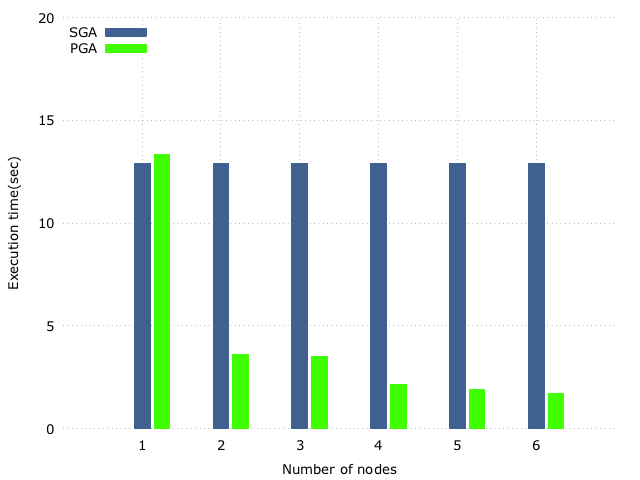
\includegraphics[width=.7 \linewidth]{stats_data_new/graphs/pga_partial_xNodes_hist.png}
  \caption{Experiment 5 - Runtime comparison SGA vs. PGA v3.}
  \end{center}\
\end{figure}

\begin{figure}[H]
\begin{center}
  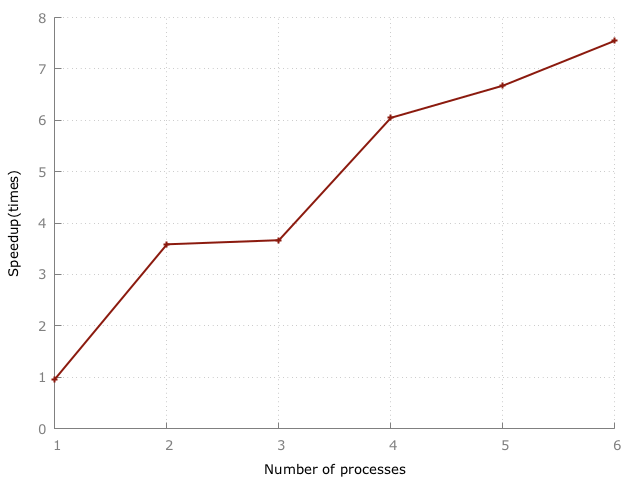
\includegraphics[width=.7 \linewidth]{stats_data_new/graphs/pga_partial_xNodes_line.png}
  \caption{Experiment 5 - Speedup graph SGA vs. PGA v3.}
  \end{center}\
\end{figure}

\subsubsection{Discussion}
In this experiment we see a better improvement in overall speedup. But the curb of the gain is not smooth. From 2 processes to 3 processes there is not much gain but from 3 processes to 4 processes we see a sudden spike. Only explanation of this could be the fact that how MPI Process Manager creates process in the cluster. With the hosts file configuration shown in Section \ref{lst:config_hydra}, Hydra (MPI Process Manager) runs 2 processes in one physical node. So, with both 3 and 4 processes we have 2 physical nodes running this program. Most likely, the underlying cache management and network overheard per node have something to do with the irregular performance variance. Running 2 processes in same physical node would have advantages of less network overheads and better caching over running a single process. This could only be confirmed by profiling this program using TAU(Tuning and Analysis Utilities) to further analyse it and find out any underlying cause should we had more time.


\subsection{Experiment 6: Varying population size}

\subsubsection{Objective}
Comparison of PGA v3 runtime vs. SGA runtime varying the number the population size using 6 processes for PGA program.

\begin{table}[H]
\centering
\caption{Experiment 6 data using PGA v2}
\label{tab:pga3_pop}
\begin{tabular}{|l|l|l|l|}
\hline
\# population & SGA     & PGA    & speedup \\ \hline
1000          & 0.5694  & 0.3594 & 1.5844  \\ \hline
2000          & 2.1434  & 0.6143 & 3.4894  \\ \hline
3000          & 4.7145  & 0.9252 & 5.0954  \\ \hline
4000          & 8.3063  & 1.3231 & 6.2777  \\ \hline
5000          & 12.9011 & 1.6985 & 7.5957  \\ \hline
6000          & 18.5207 & 2.2113 & 8.3753  \\ \hline
7000          & 25.1309 & 2.7727 & 9.0636  \\ \hline
8000          & 32.6705 & 3.4446 & 9.4846  \\ \hline
9000          & 41.2867 & 4.2053 & 9.8179  \\ \hline
10000         & 50.9591 & 5.0311 & 10.1288 \\ \hline
\end{tabular}
\end{table}

\begin{figure}[H]
\begin{center}
  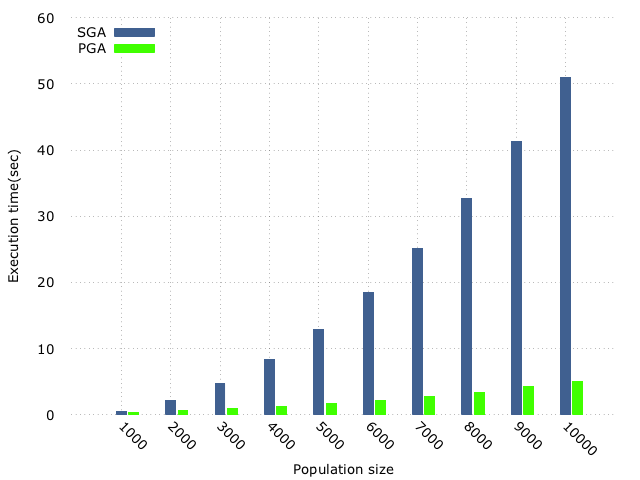
\includegraphics[width=.7 \linewidth]{stats_data_new/graphs/pga_partial_xPop_hist.png}
  \caption{Experiment 6 - Runtime comparison SGA vs. PGA v3.}
  \end{center}\
\end{figure}

\begin{figure}[H]
\begin{center}
  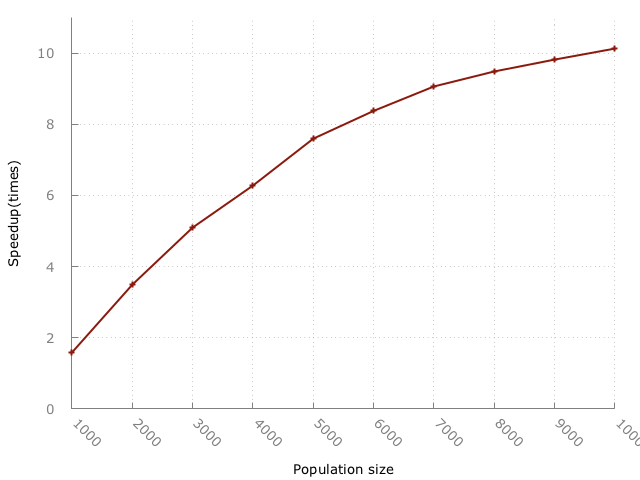
\includegraphics[width=.7 \linewidth]{stats_data_new/graphs/pga_partial_xPop_line.png}
  \caption{Experiment 6 - Speedup graph SGA vs. PGA v3.}
  \end{center}\
\end{figure}

\subsubsection{Discussion}
With this experiment we can see there is a consistent speedup gain with PGA v3 compared to the SGA program as population size is increased. Even though the outcome of this experiment is as expected, the results are taken as speculative until further experiments are done using different parameters. Profiling of this program also needs to be done to see a consistent and reliable outcome.

\chapter{Conclusions}
\label{conclusions}
This project was set out to implement a parallel GA using MPI and profiling the performance issue over a sequential version by varying the number of parallel processes and population size. Initially, we expected to see a substantial performance gain by parallelising the SGA. By implementing the Parallel GA many underlying issues and techniques were discovered that were unknown to me previously. 

In MPI the communication cost is major concern. If a program is not carefully designed to minimise the communication overhead the overall performance can suffer a lot. As we have discovered, there are three very different models of parallel GA. Out of these three only the first model(Master-slave) implemented in this project. The experiments done in this project shown that the traditional master-slave model of PGA using MPI does not result in much performance gain over the sequential SGA because of the communication cost involved for message-passing. In general MPI programs are more suitable for computationally heavy program. If the computational cost is not greater than the communication cost then its performance gain will be negative. The subsequent versions of the PGA (v3), the GA behaviour was changed due to the fact that it is very close to \textit{Island} model. This model of parallel GA needs a migration policy implemented. The time constraint was a major factor for this challenging project. If time permitted, the next step would be to implement a distributed model of Parallel GA with a migration policy.


This project was an exploratory experience in using MPI library and a Cluster computing environment. In this project I have had a great experience in exploring many difficult and exciting concepts in Parallelisation, High Performance Computing(HPC) and some aspect of Genetic Algorithms(GA). I have learned the advantages and limitation of MPI libraries and many underlying challenging issues involved. I gained a lot of experience in setting up a Beowulf cluster, configuring and administration of Linux Server, using remote development environment and shell scripting. Last but not least learned to use \LaTeX\  to produce this report. 

%\bibliographystyle{unsrtnat}
\bibliographystyle{agsm}
\bibliography{references}

\begin{appendices}
\chapter{Project plans}
\label{appendix:project_plans}
\begin{figure}[!htb]
  \center
  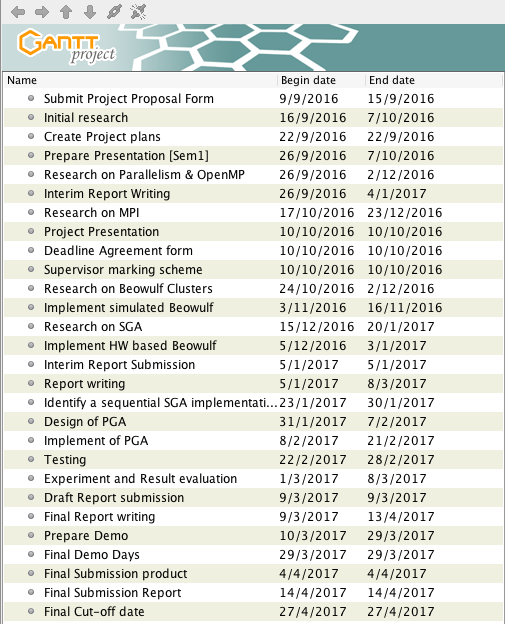
\includegraphics[width=.7 \linewidth]{figs/project_plans_list.png}
  \caption{Gantt Project plans - List}
  \label{fig:project_plans}
\end{figure}

\begin{figure}[!htb]
  \center
  \includegraphics[width=.7 \linewidth]{figs/FYP_Project_plans_rotated.png}
  \caption{Gantt Project plans - Graph}
  \label{fig:project_plans}
\end{figure}

\chapter{Git logs}
\begin{figure}[!htb]
  \center
  \includegraphics[width=\linewidth]{figs/git_logs.png}
  \caption{PGA Version control logs.}
  \label{fig:git_logs}
\end{figure}


\chapter{Project source codes}
\label{sourcecodes}
\section{params.hpp}
\label{src:params.hpp}
\lstinputlisting[language=c]{src_codes/params.hpp}

\section{sga\_proc.hpp}
\label{src:sga_proc.hpp}
\lstinputlisting[language=c]{src_codes/sga_proc.hpp}

\section{sga.cpp}
\label{src:sga.cpp}
\lstinputlisting[language=c]{src_codes/sga.cpp}

\section{pga\_proc.hpp}
\label{src:pga_proc.hpp}
\lstinputlisting[language=c]{src_codes/pga_proc.hpp}

\section{pga.cpp}
\label{src:pga.cpp}
\lstinputlisting[language=c]{src_codes/pga.cpp}

\section{pgav2.cpp}
\label{src:pgav2cpp}
\lstinputlisting[language=c]{src_codes/pgav2.cpp}

\section{sga\_proc.cpp}
\label{src:sga_proc.cpp}
\lstinputlisting[language=c]{src_codes/sga_proc.cpp}

\section{pga\_proc.cpp}
\label{src:pga_proc.cpp}
\lstinputlisting[language=c]{src_codes/pga_proc.cpp}


\end{appendices}

\end{document}   


